\section{Anhang}
Im folgenden sind die Peaks 1 bis 22 der Messdaten mit vorgegebenem Pulver und dem Fit mit einem Chiquadrat von 22 zu sehen.
\begin{figure}[H]
\begin{minipage}{.5\textwidth}
  \centering
  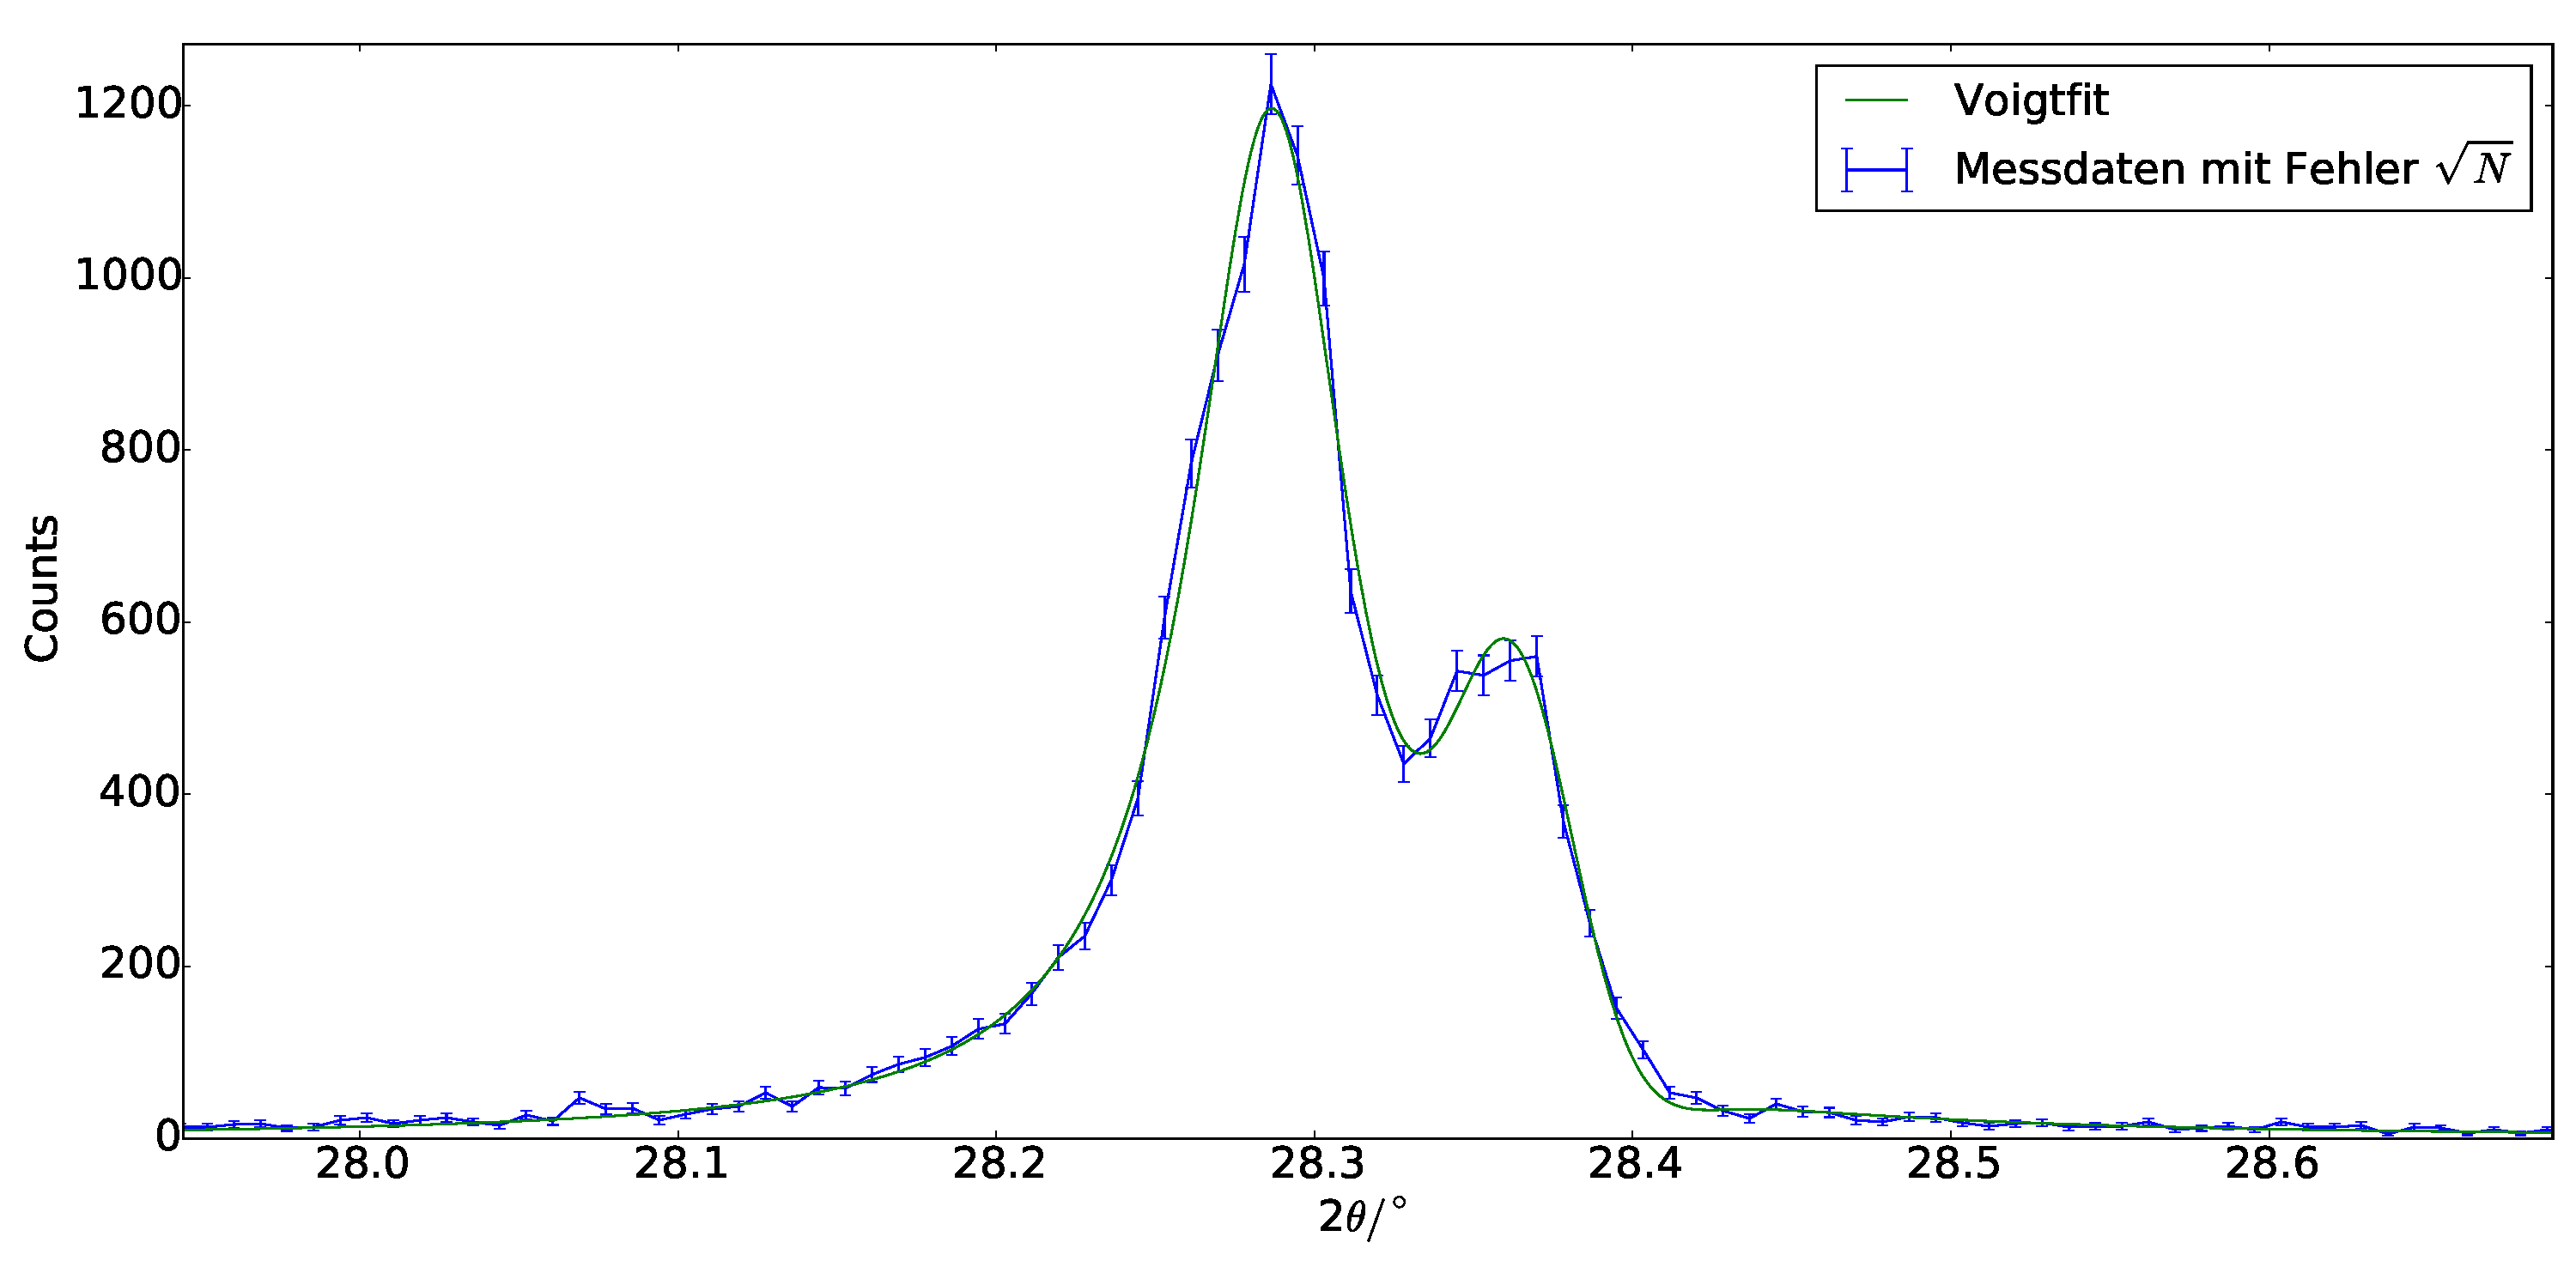
\includegraphics[scale=0.15]{messung_pulver_1}
  \captionof{figure}{Pulverdaten 1. Doppelpeak}
  \label{fig:pul_mess_1}
\end{minipage}
\hspace{0.5cm}
\begin{minipage}{.5\textwidth}
  \centering
  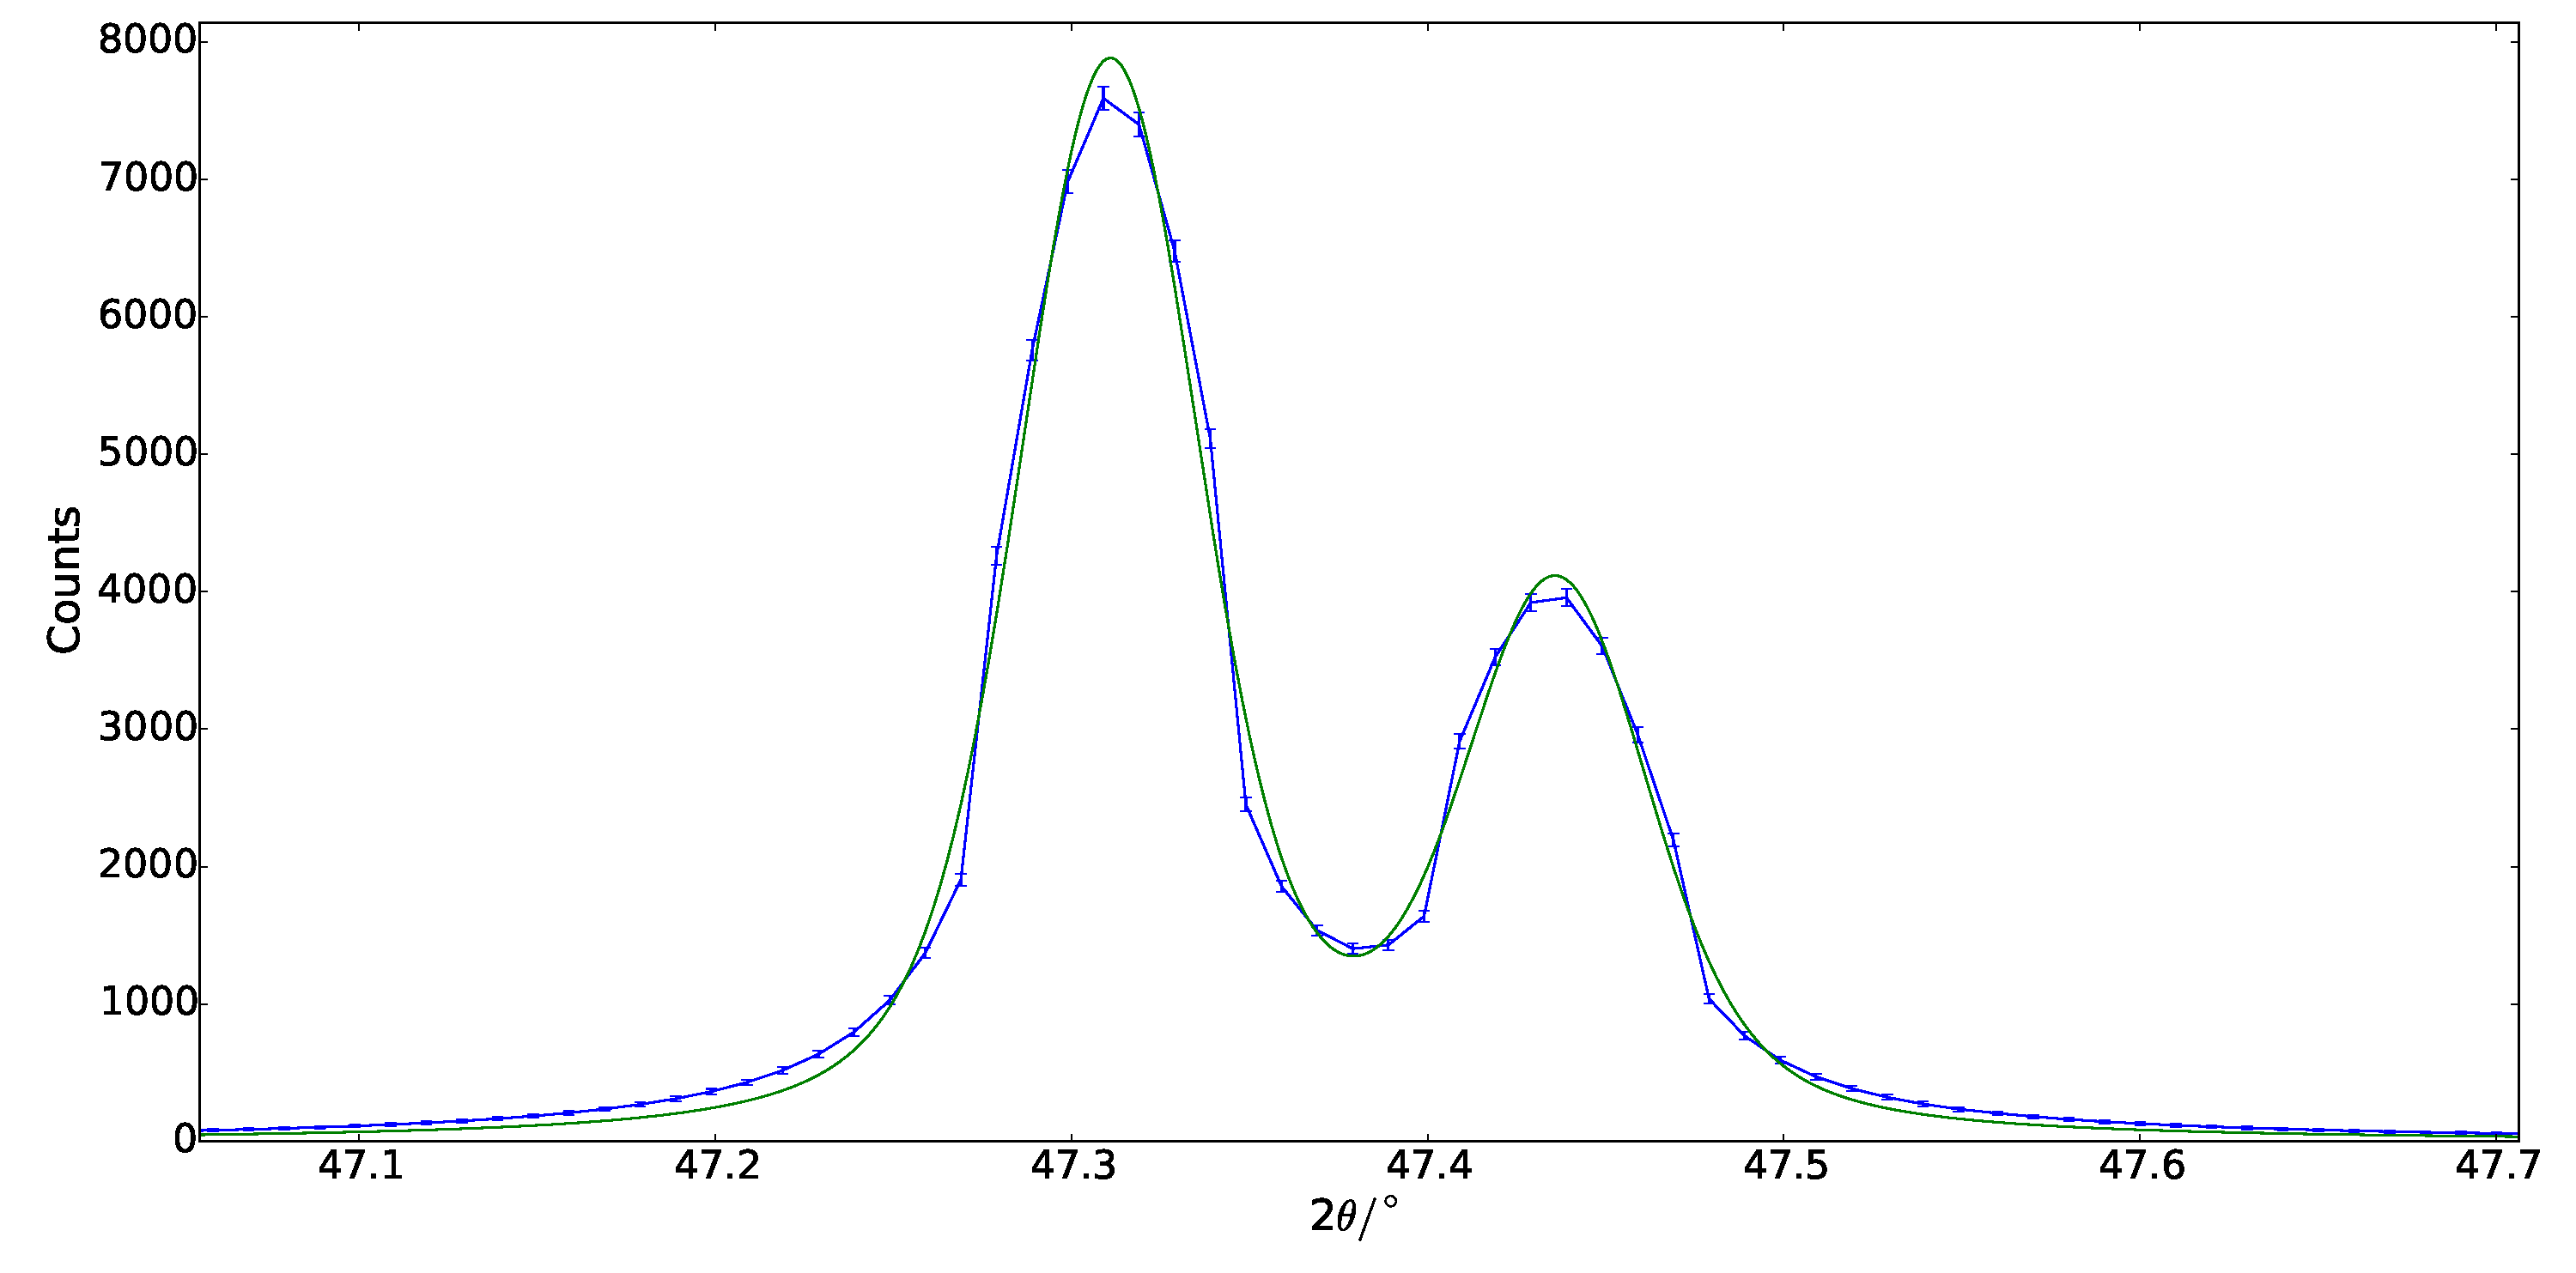
\includegraphics[scale=0.15]{messung_pulver_2}
  \captionof{figure}{Pulverdaten 2. Doppelpeak}
  \label{fig:pul_mess_2}
\end{minipage}
\end{figure}
\begin{figure}[H]
\begin{minipage}{.5\textwidth}
  \centering
  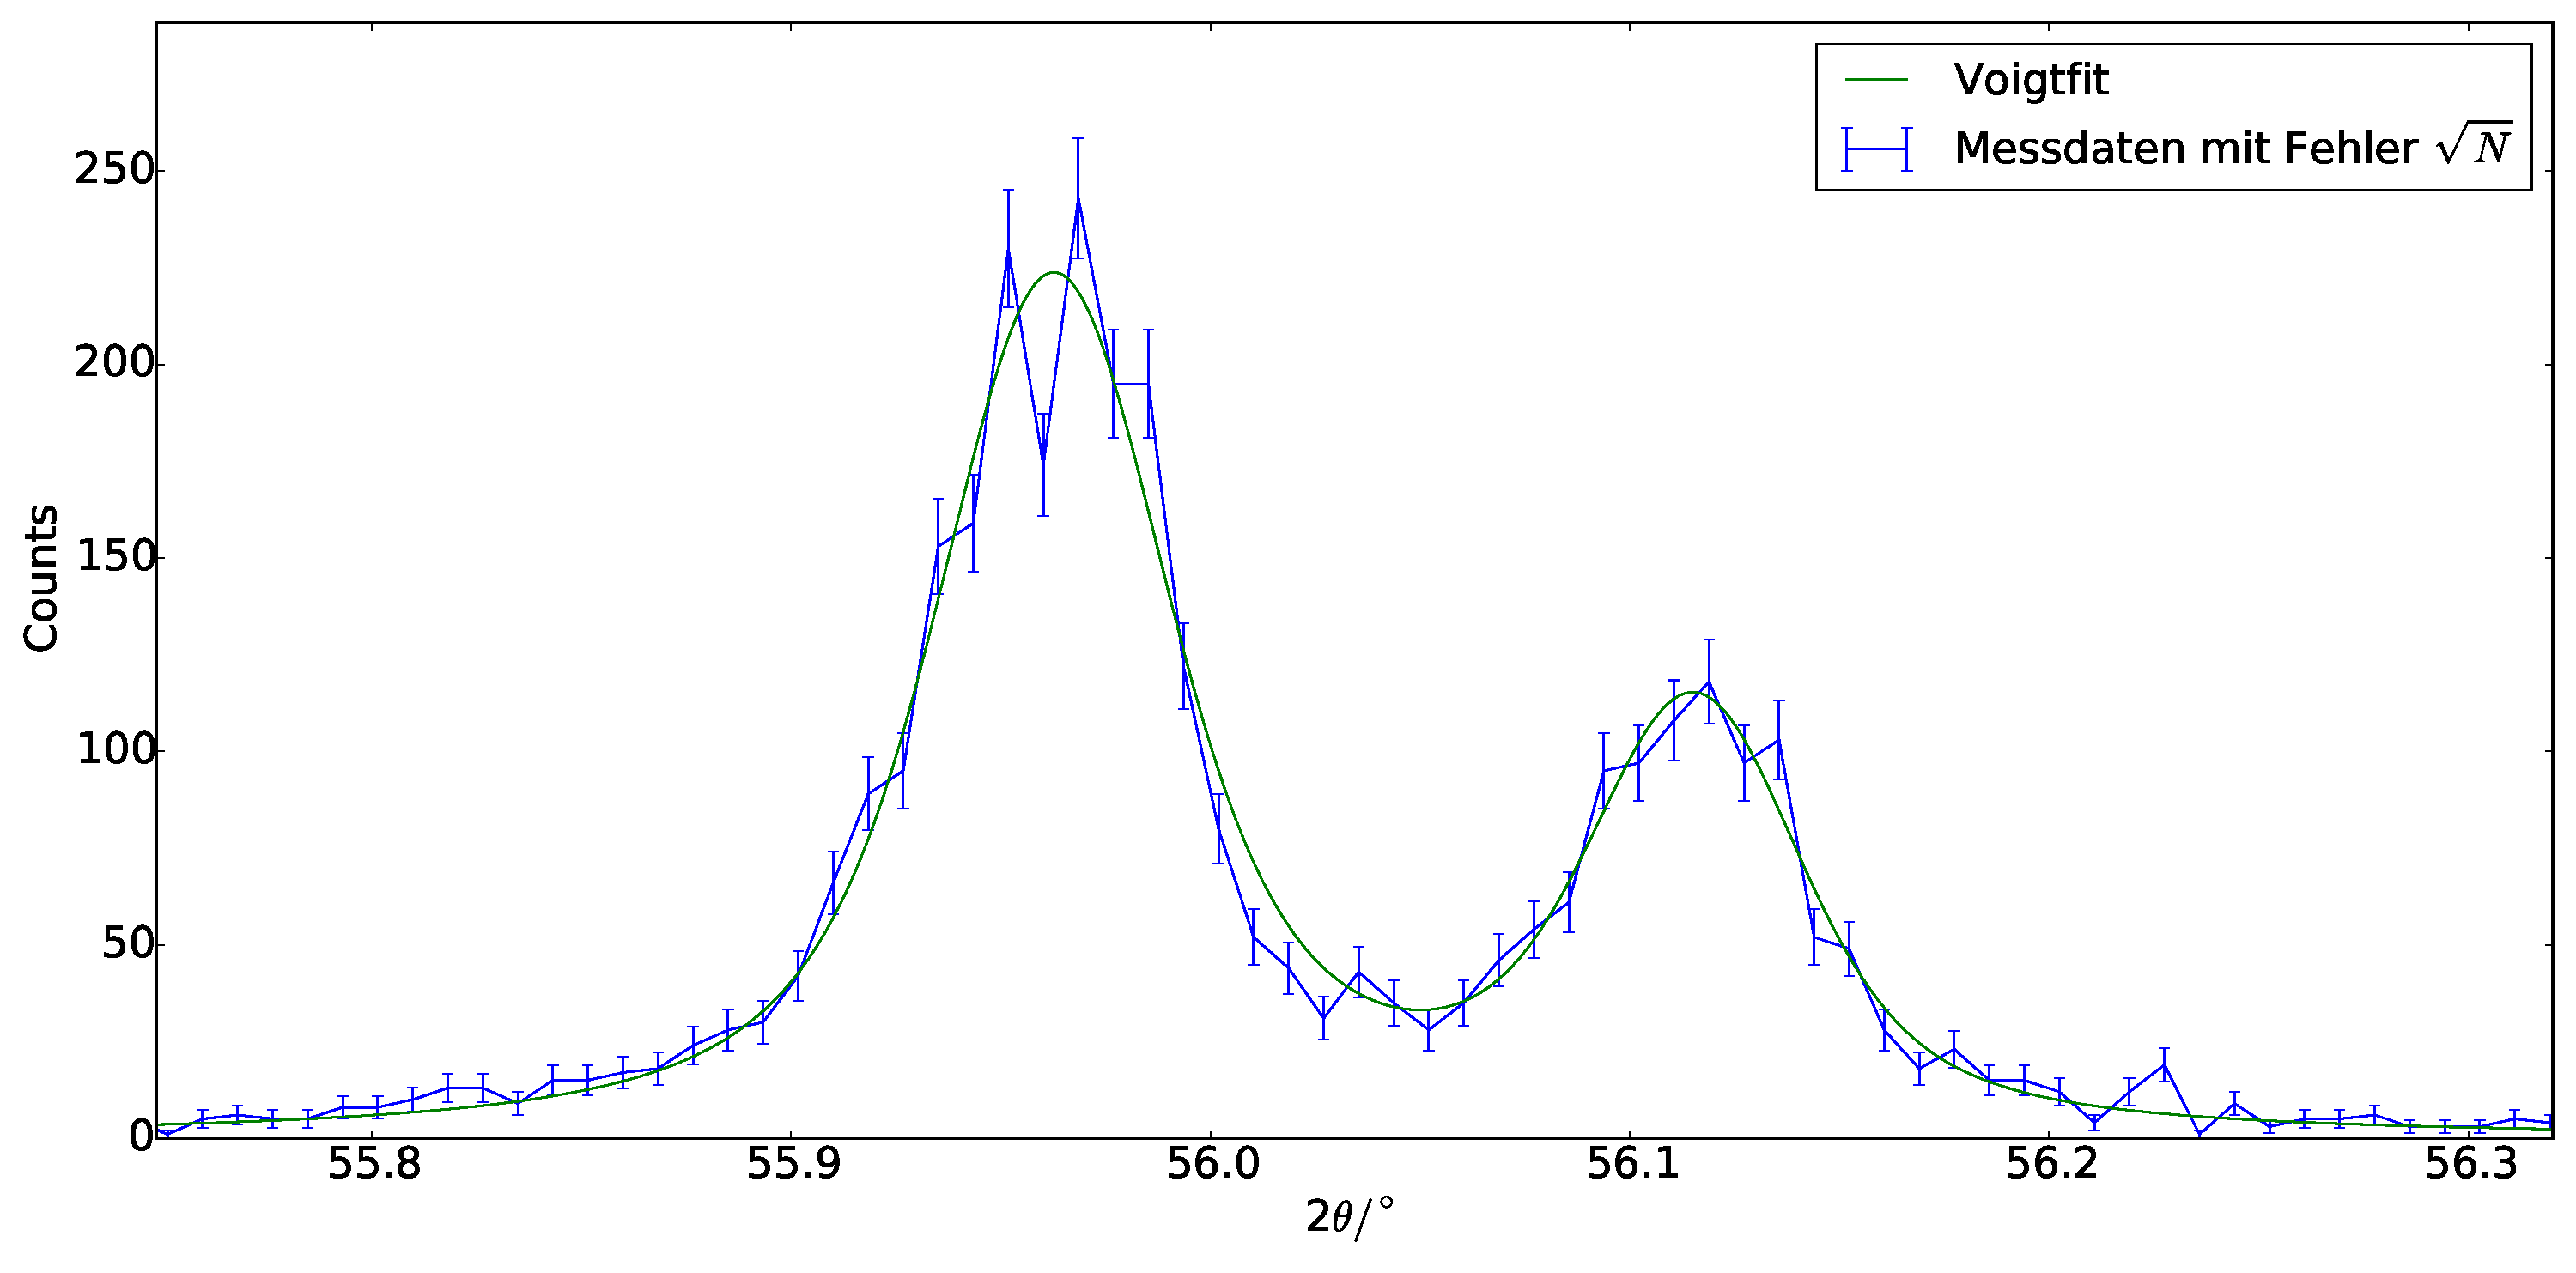
\includegraphics[scale=0.15]{messung_pulver_3}
  \captionof{figure}{Pulverdaten 3. Doppelpeak}
  \label{fig:pul_mess_3}
\end{minipage}
\hspace{0.5cm}
\begin{minipage}{.5\textwidth}
  \centering
  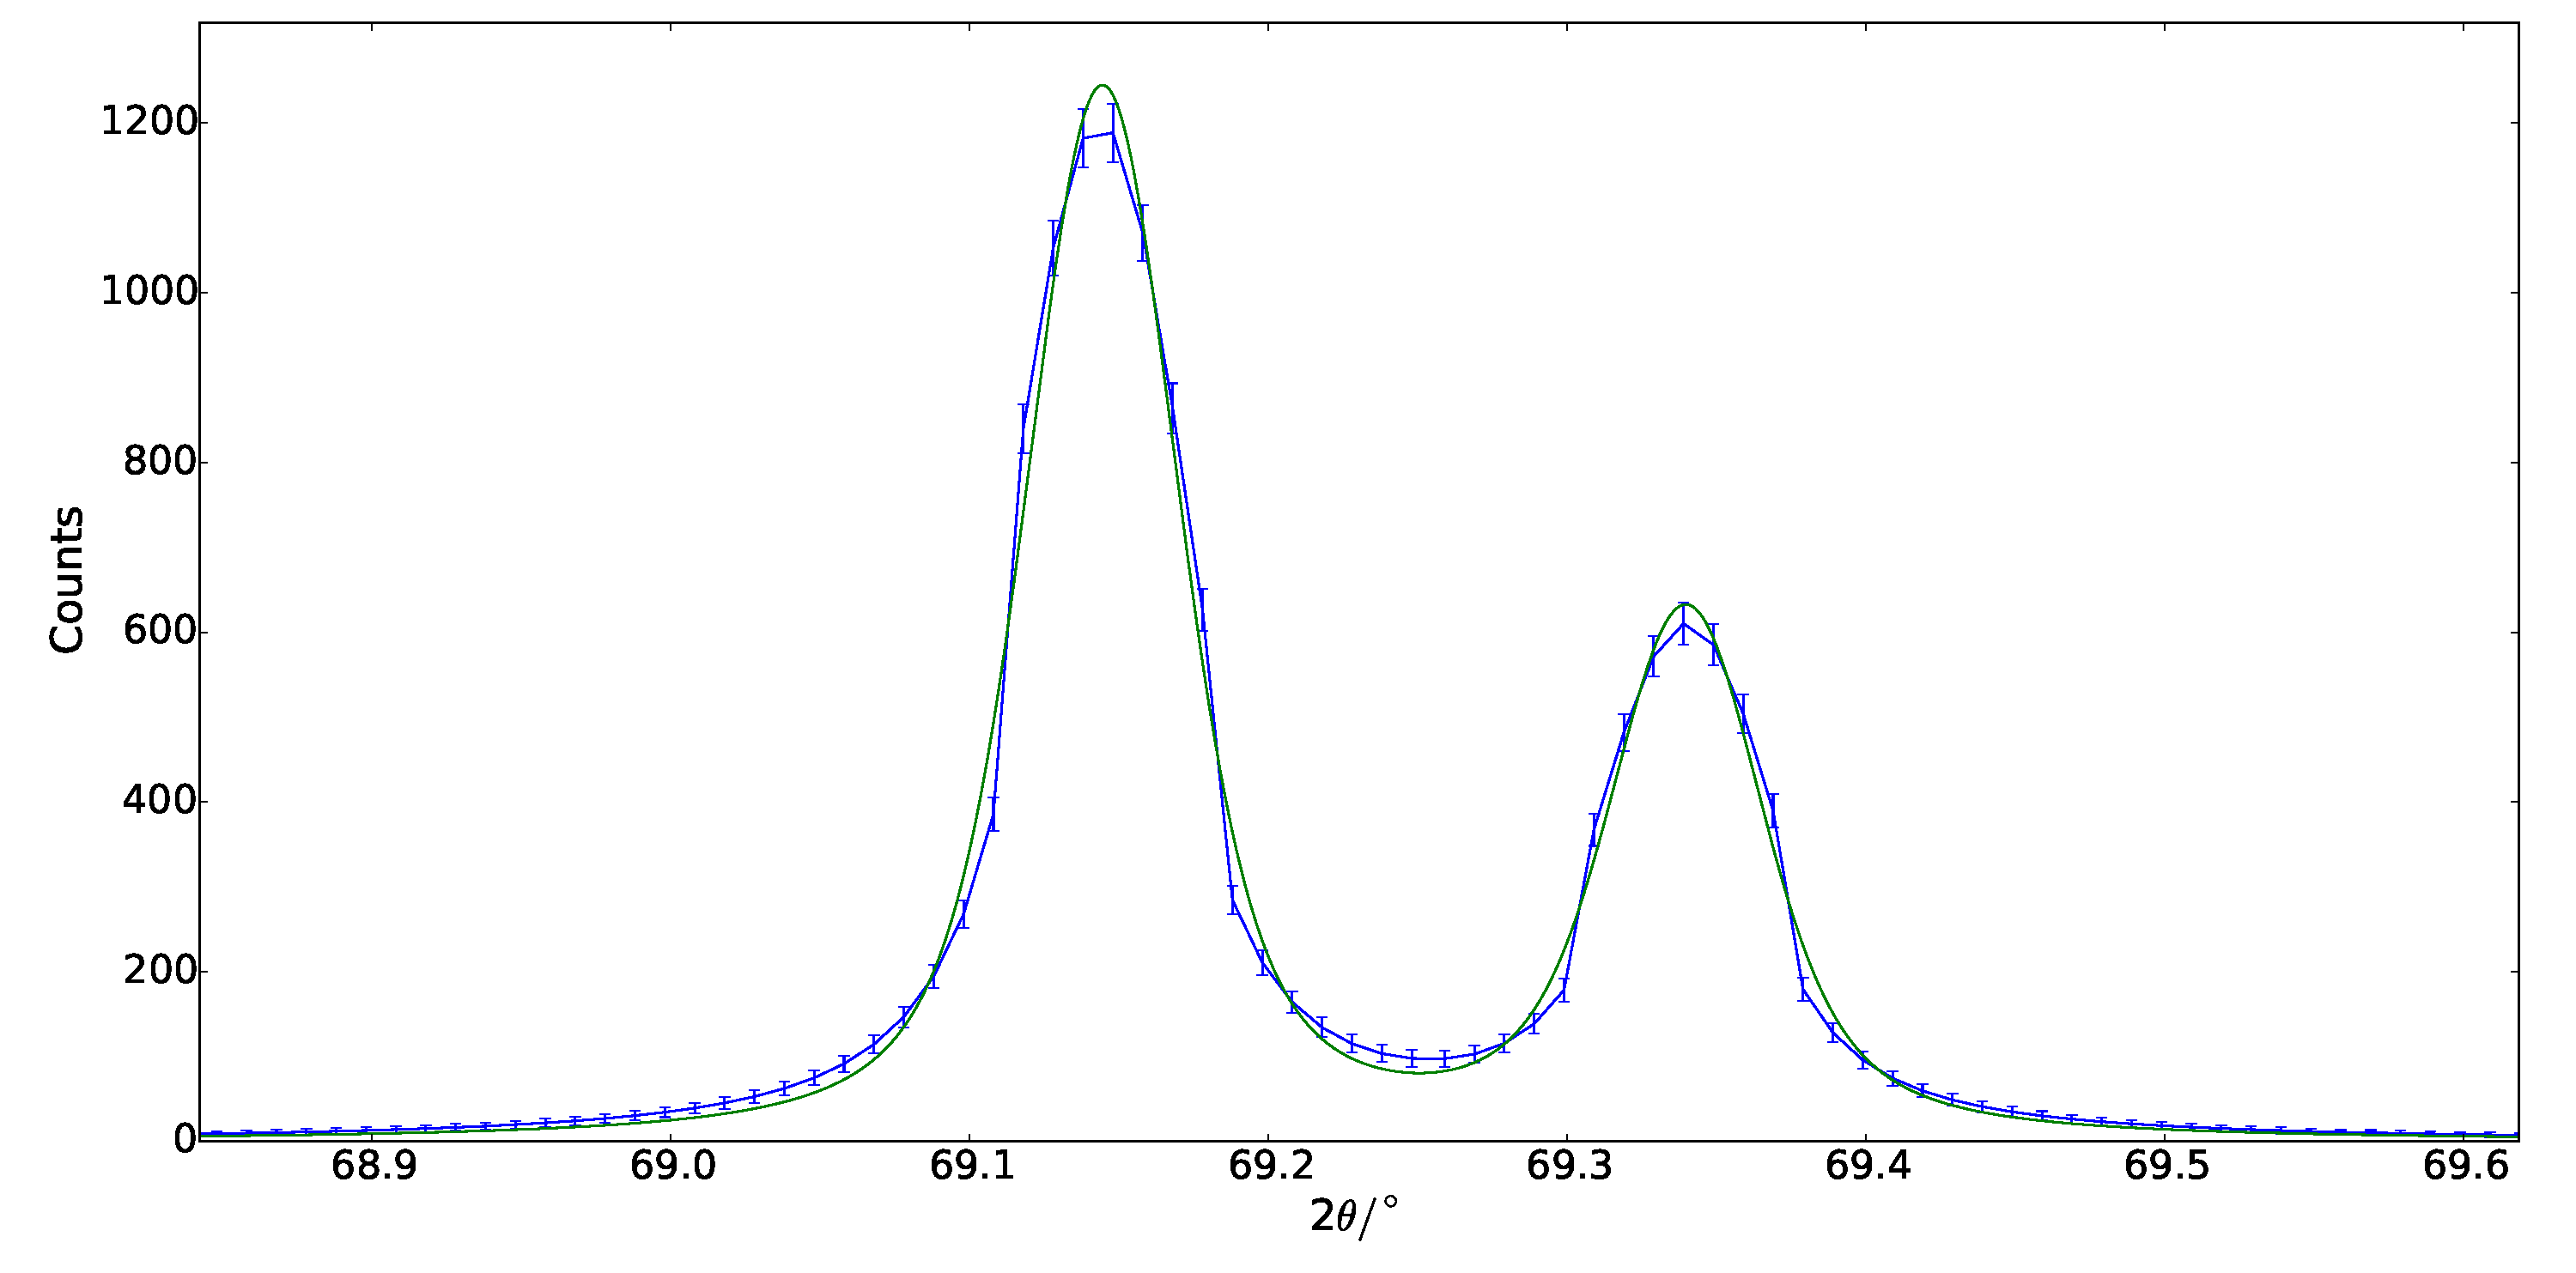
\includegraphics[scale=0.15]{messung_pulver_4}
  \captionof{figure}{Pulverdaten 4. Doppelpeak}
  \label{fig:pul_mess_4}
\end{minipage}
\end{figure}
\begin{figure}[H]
\begin{minipage}{.5\textwidth}
  \centering
  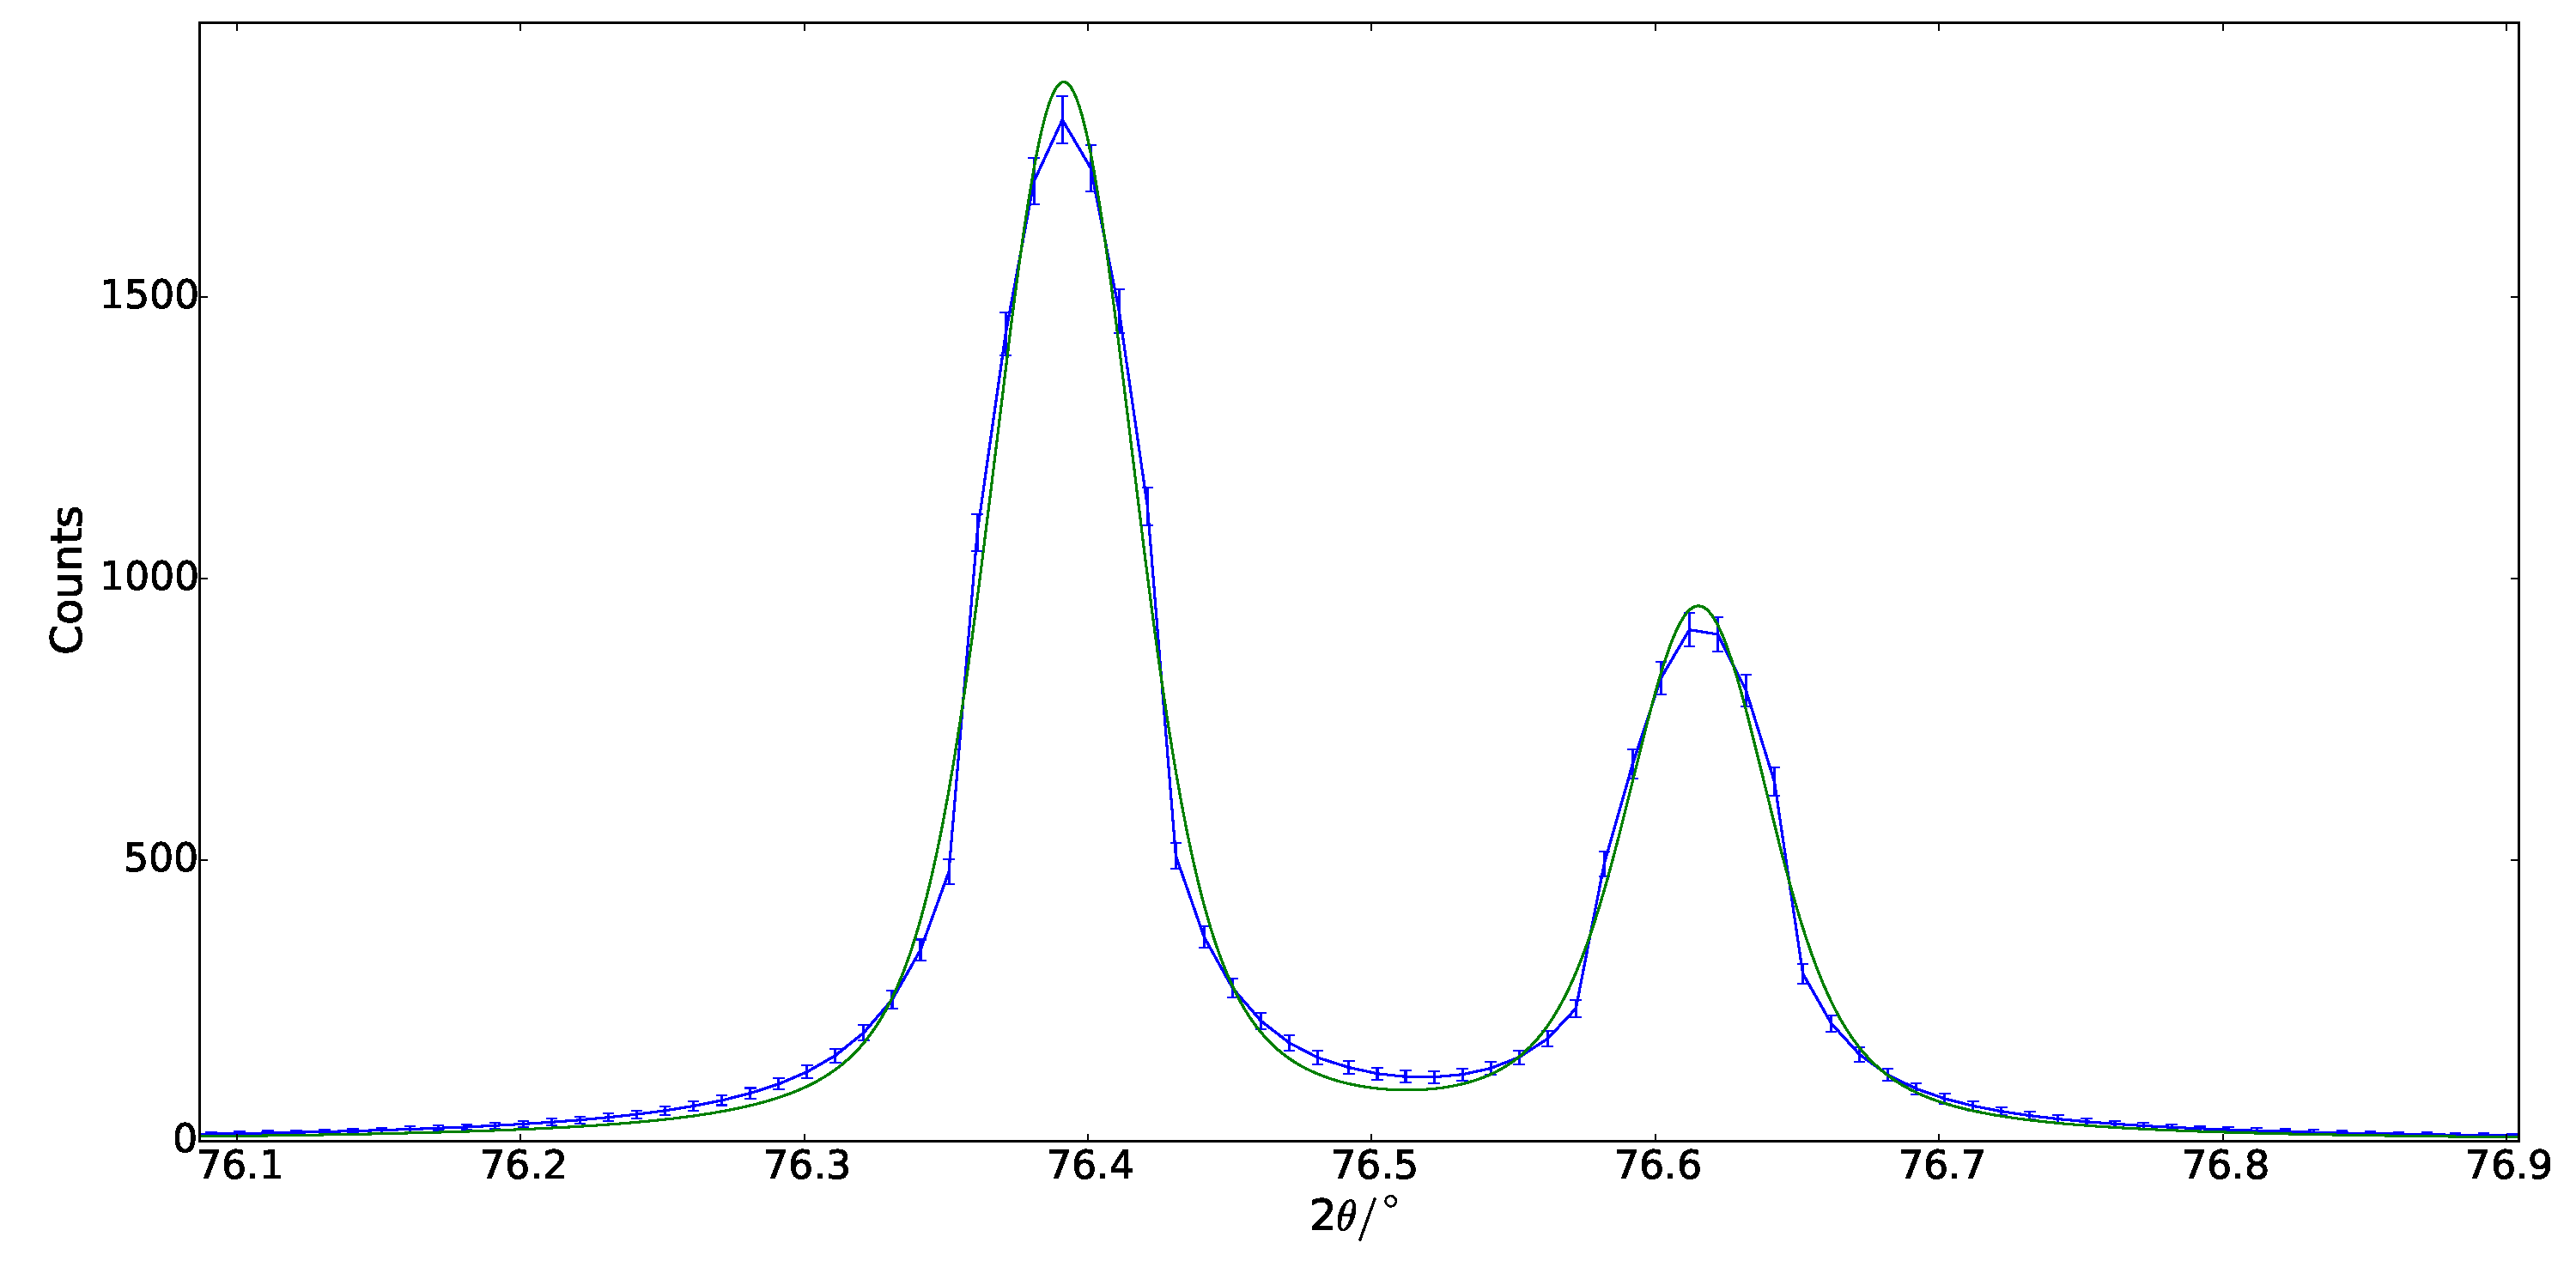
\includegraphics[scale=0.15]{messung_pulver_5}
  \captionof{figure}{Pulverdaten 5. Doppelpeak}
  \label{fig:pul_mess_5}
\end{minipage}
\hspace{0.5cm}
\begin{minipage}{.5\textwidth}
  \centering
  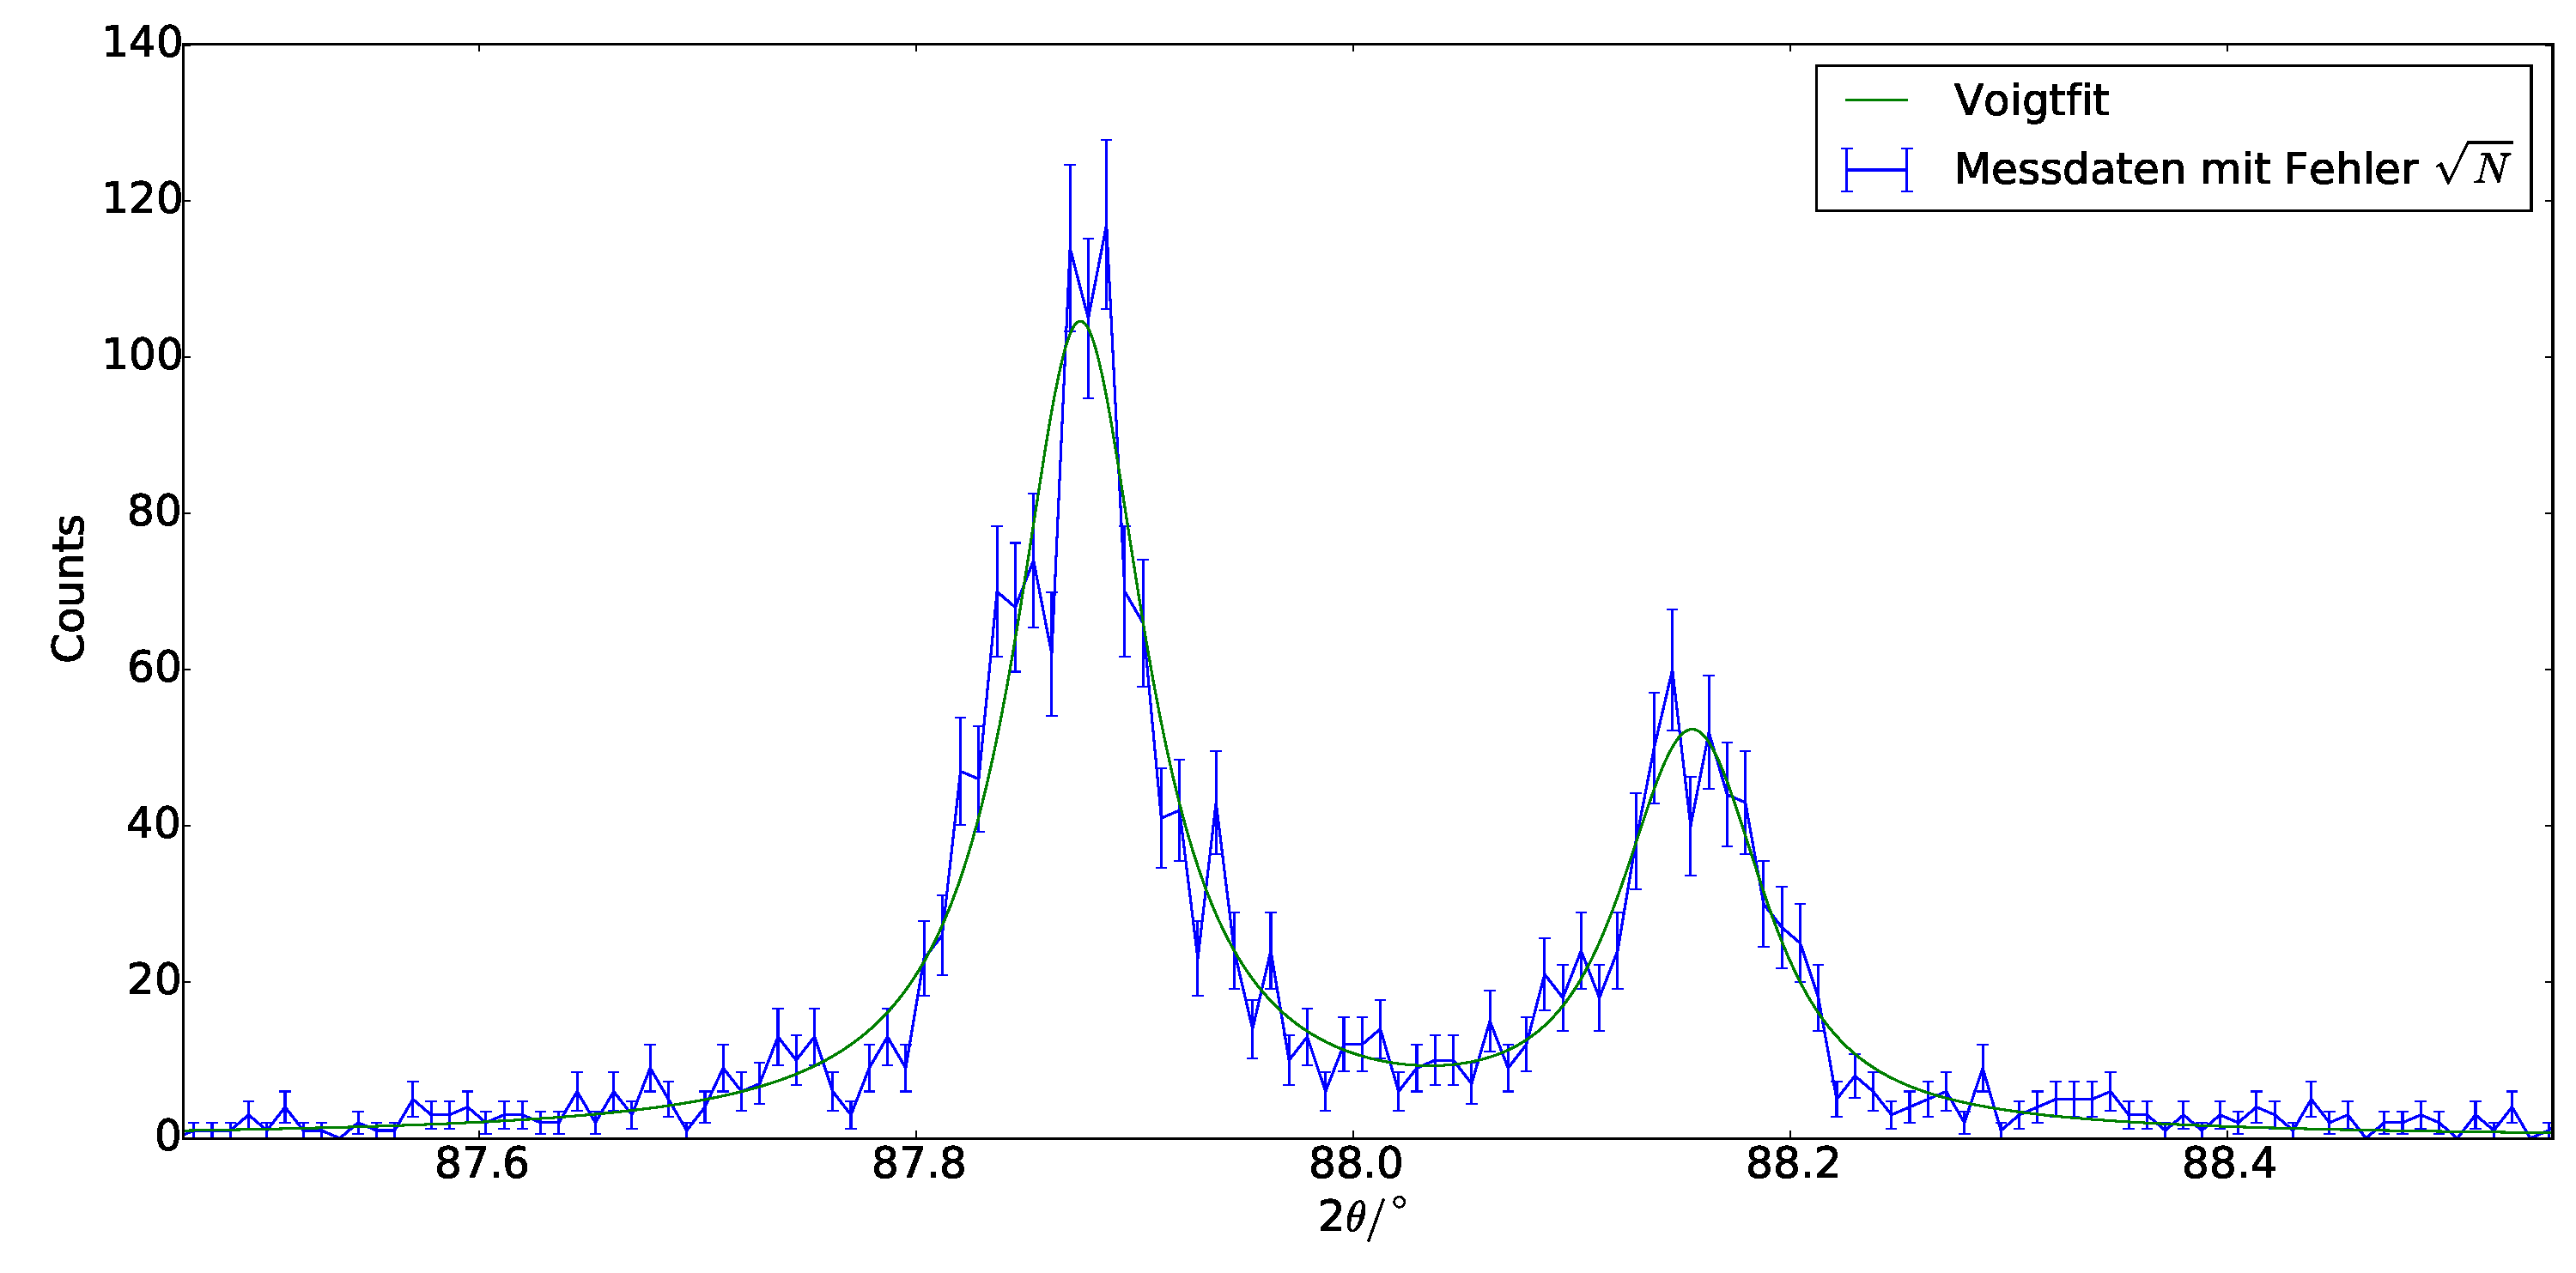
\includegraphics[scale=0.15]{messung_pulver_6}
  \captionof{figure}{Pulverdaten 6. Doppelpeak}
  \label{fig:pul_mess_6}
\end{minipage}
\end{figure}
\begin{figure}[H]
\begin{minipage}{.5\textwidth}
  \centering
  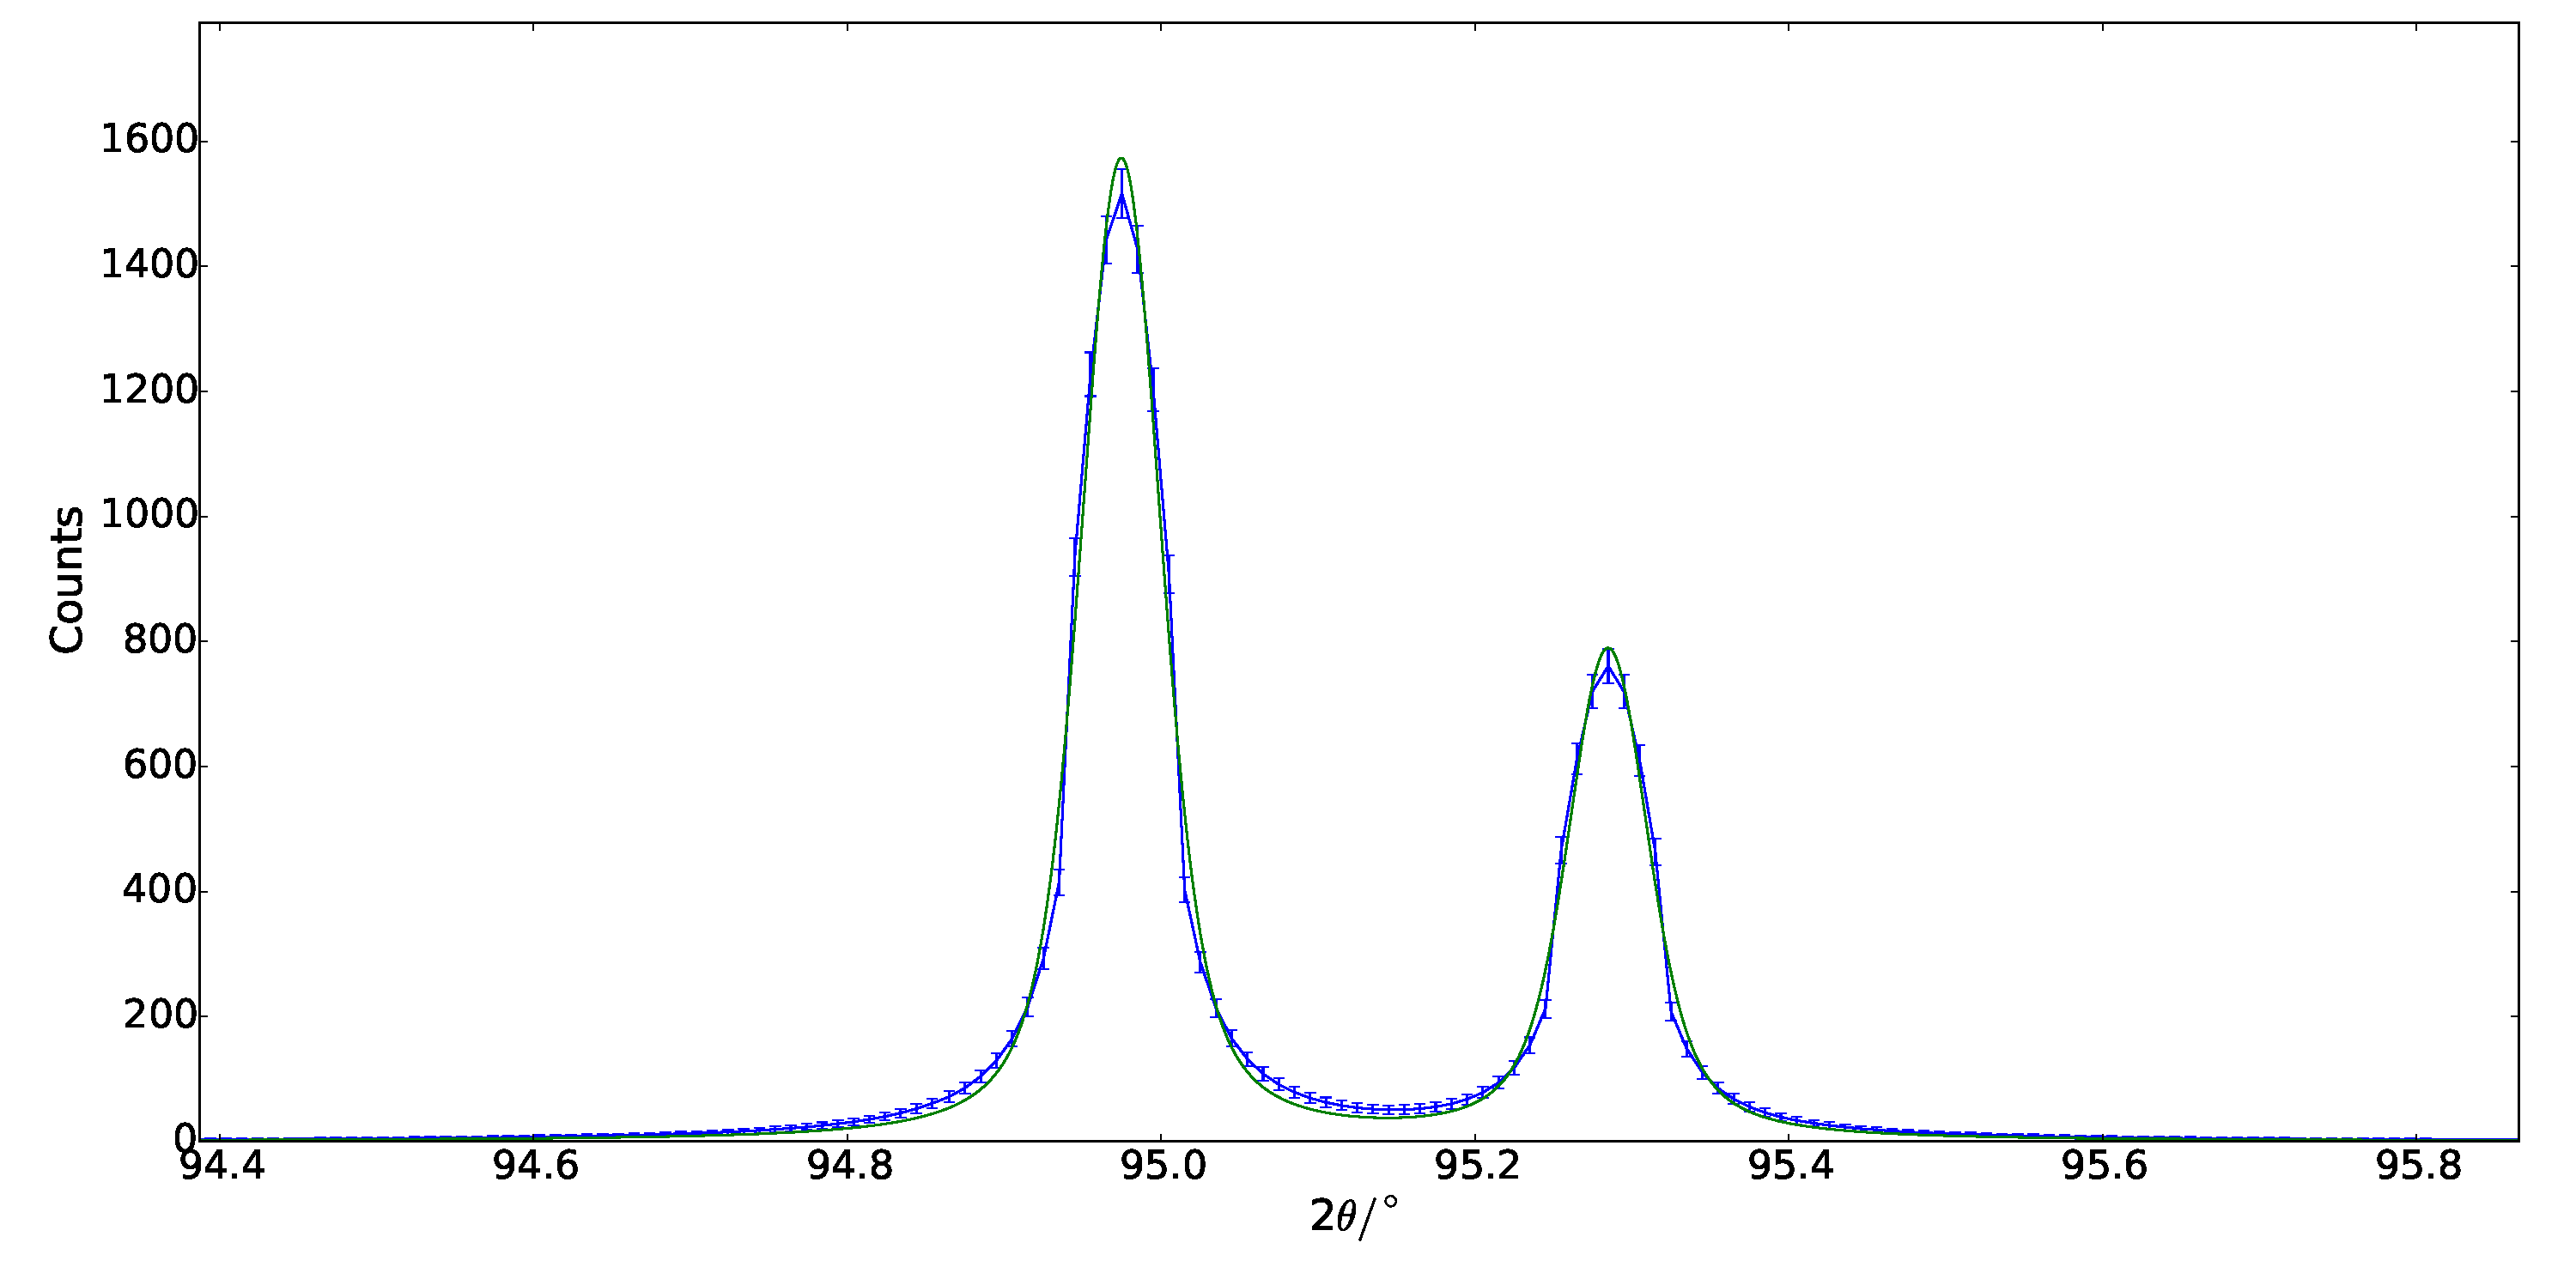
\includegraphics[scale=0.15]{messung_pulver_7}
  \captionof{figure}{Pulverdaten 7. Doppelpeak}
  \label{fig:pul_mess_7}
\end{minipage}
\hspace{0.5cm}
\begin{minipage}{.5\textwidth}
  \centering
  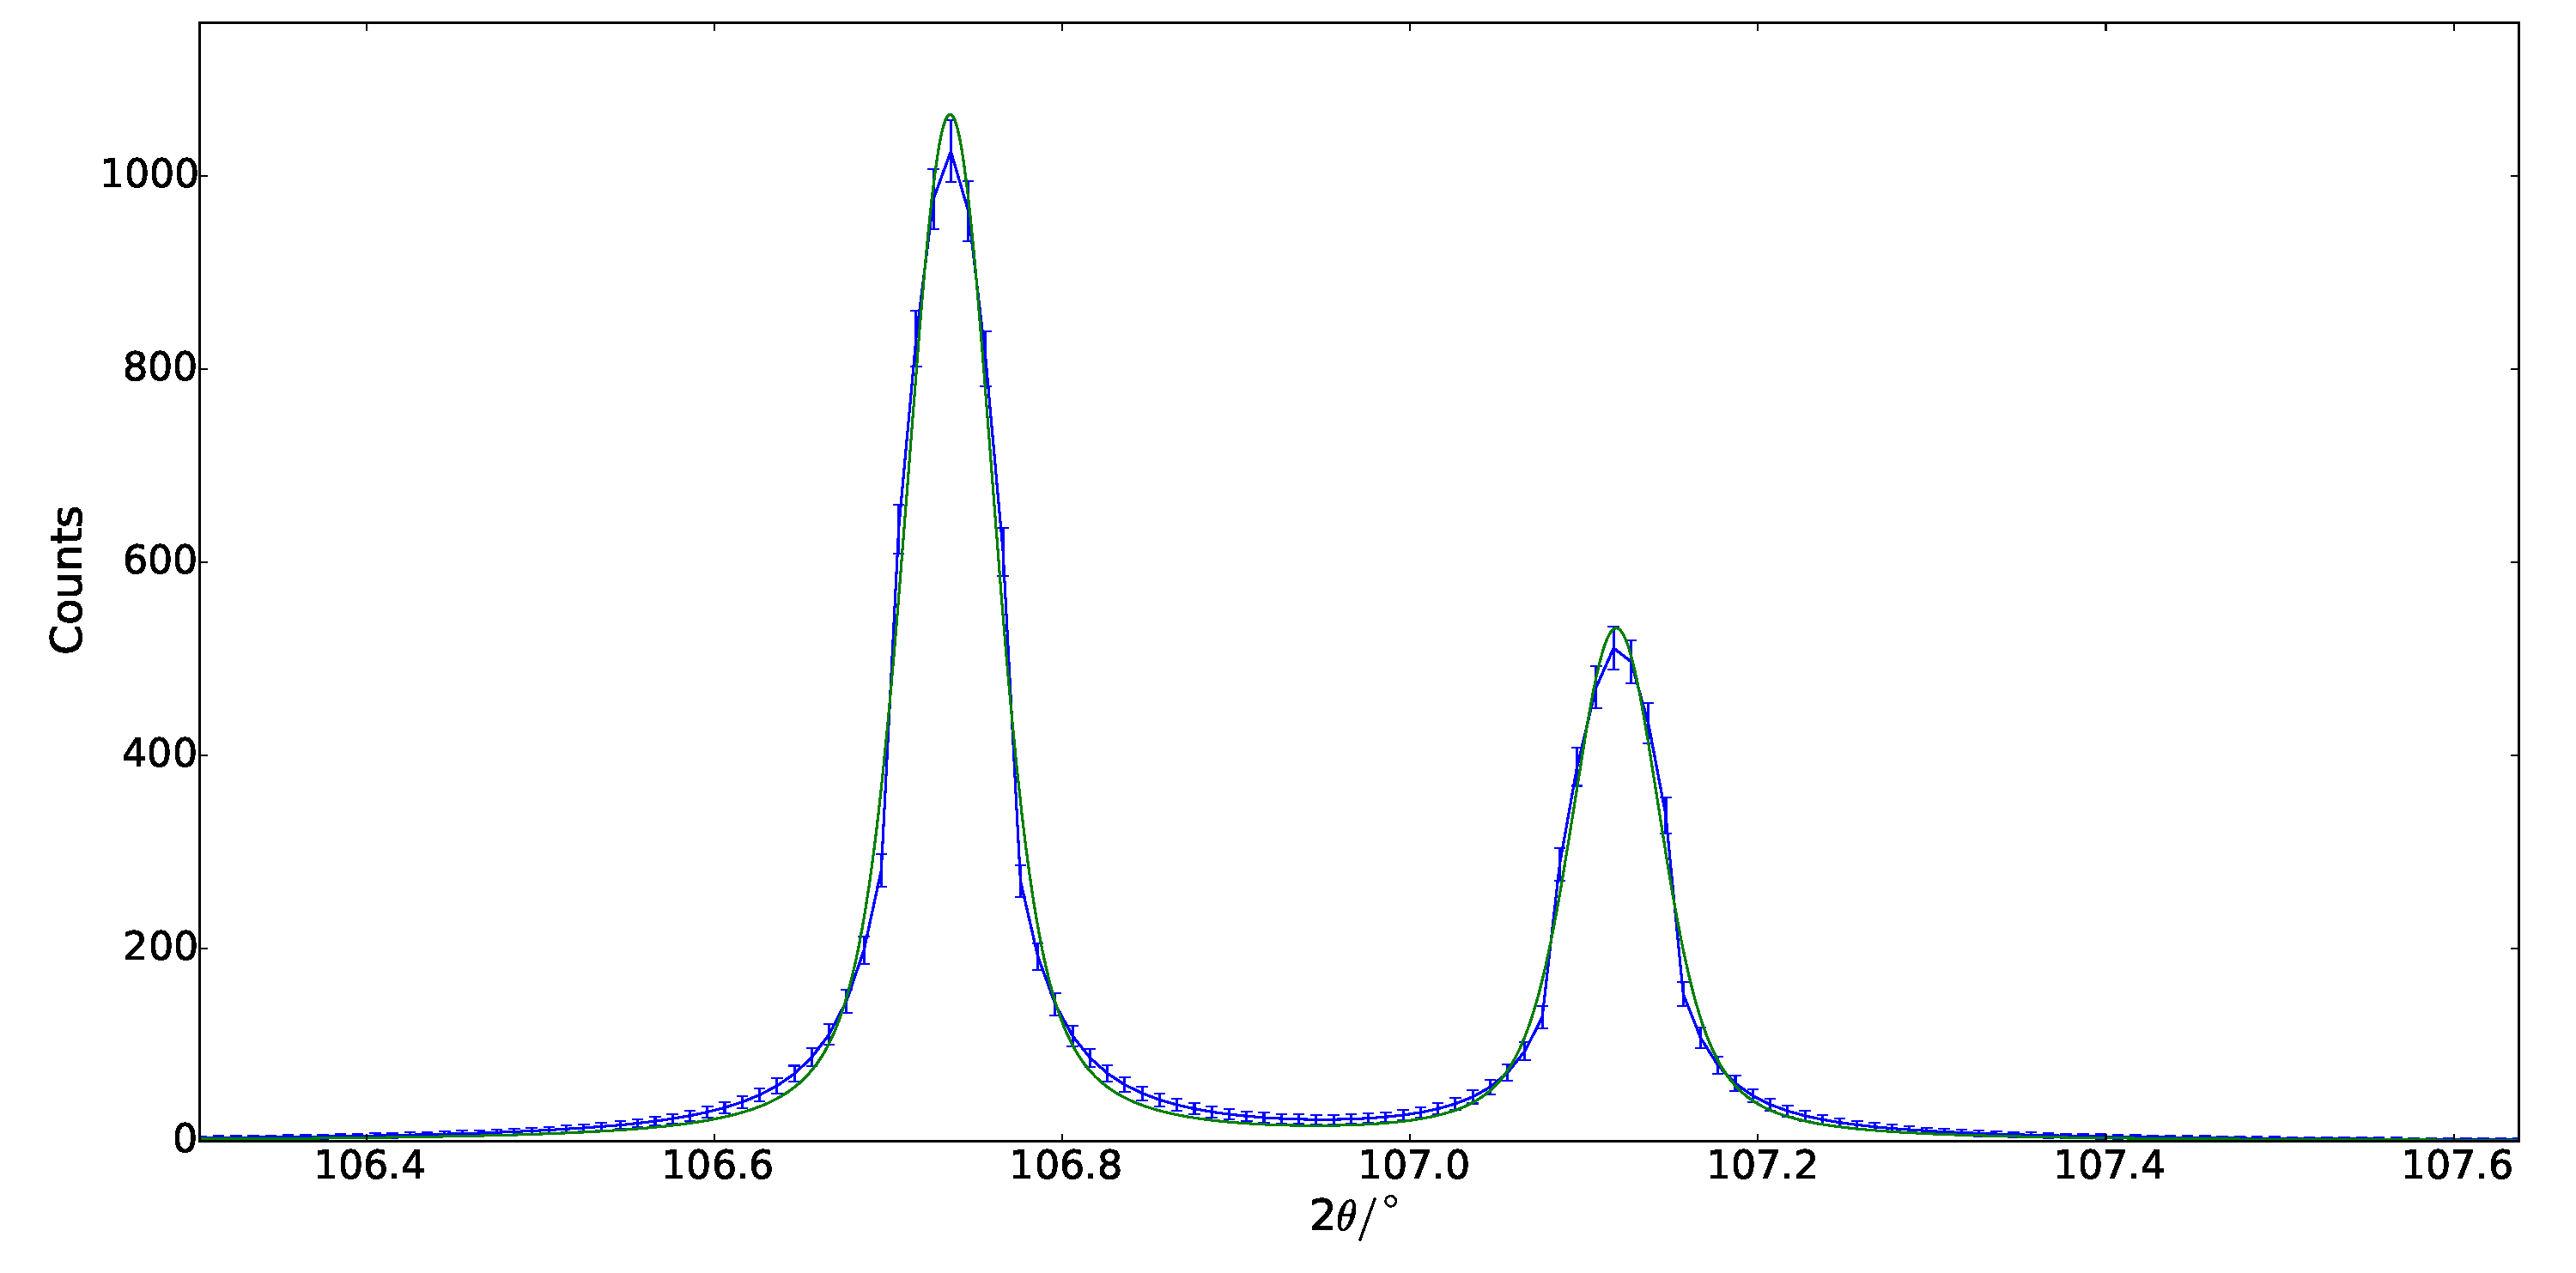
\includegraphics[scale=0.15]{messung_pulver_8}
  \captionof{figure}{Pulverdaten 8. Doppelpeak}
  \label{fig:pul_mess_8}
\end{minipage}
\end{figure}
\begin{figure}[H]
\begin{minipage}{.5\textwidth}
  \centering
  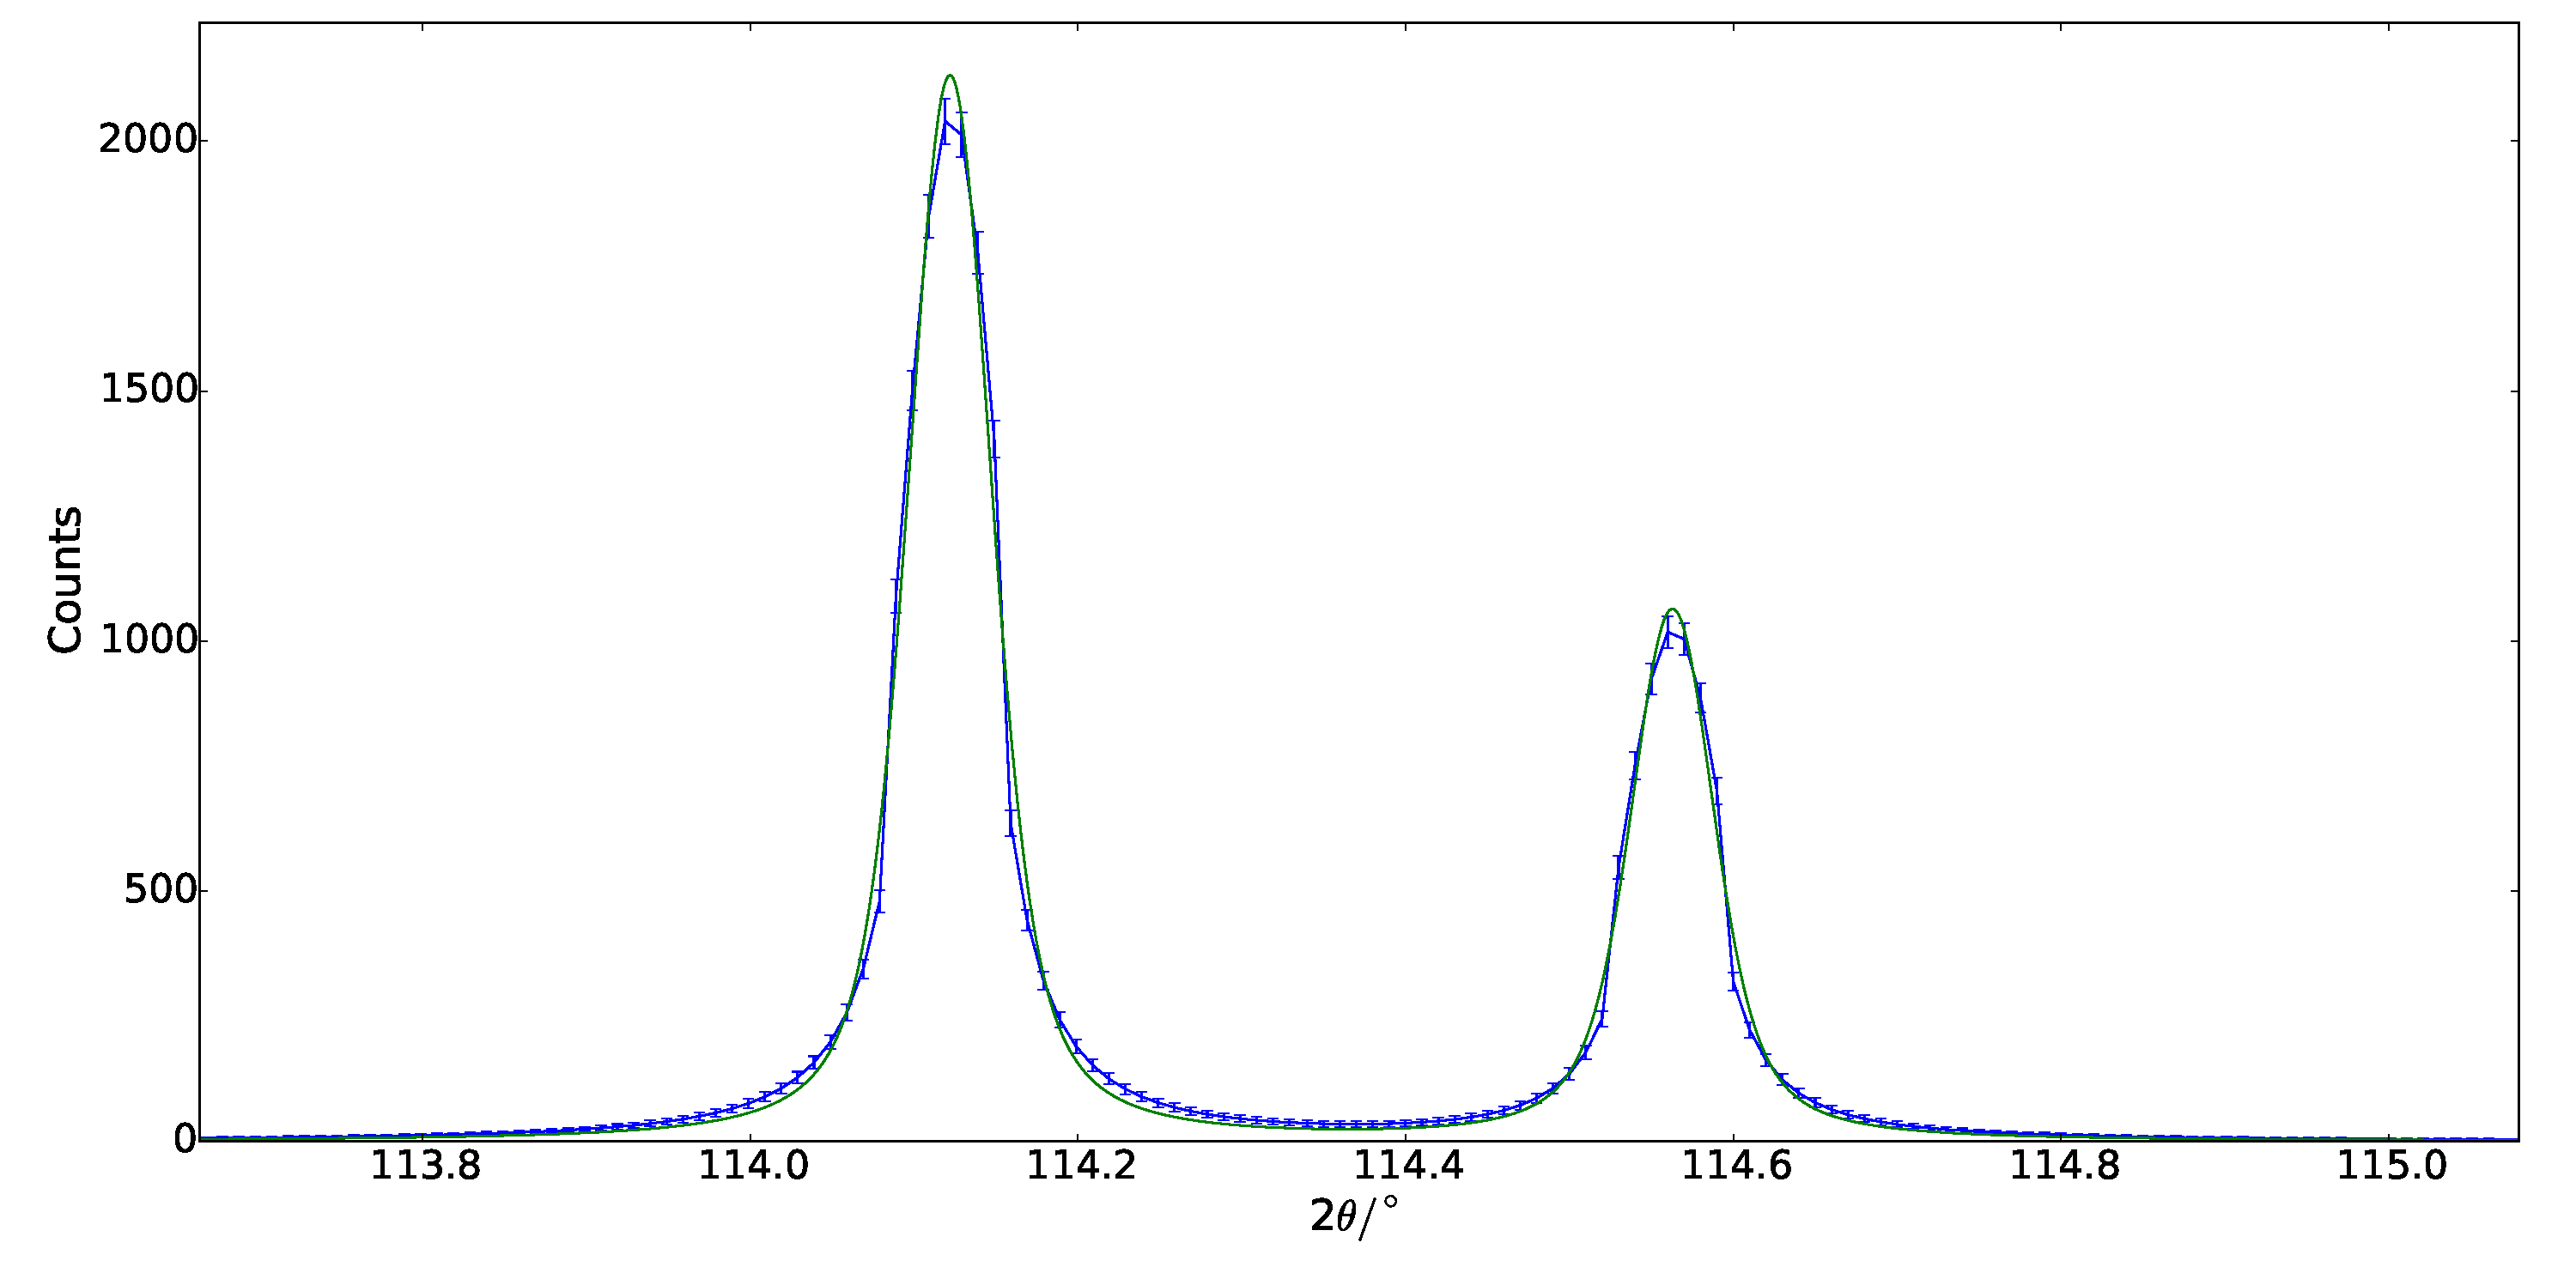
\includegraphics[scale=0.15]{messung_pulver_9}
  \captionof{figure}{Pulverdaten 9. Doppelpeak}
  \label{fig:pul_mess_9}
\end{minipage}
\hspace{0.5cm}
\begin{minipage}{.5\textwidth}
  \centering
  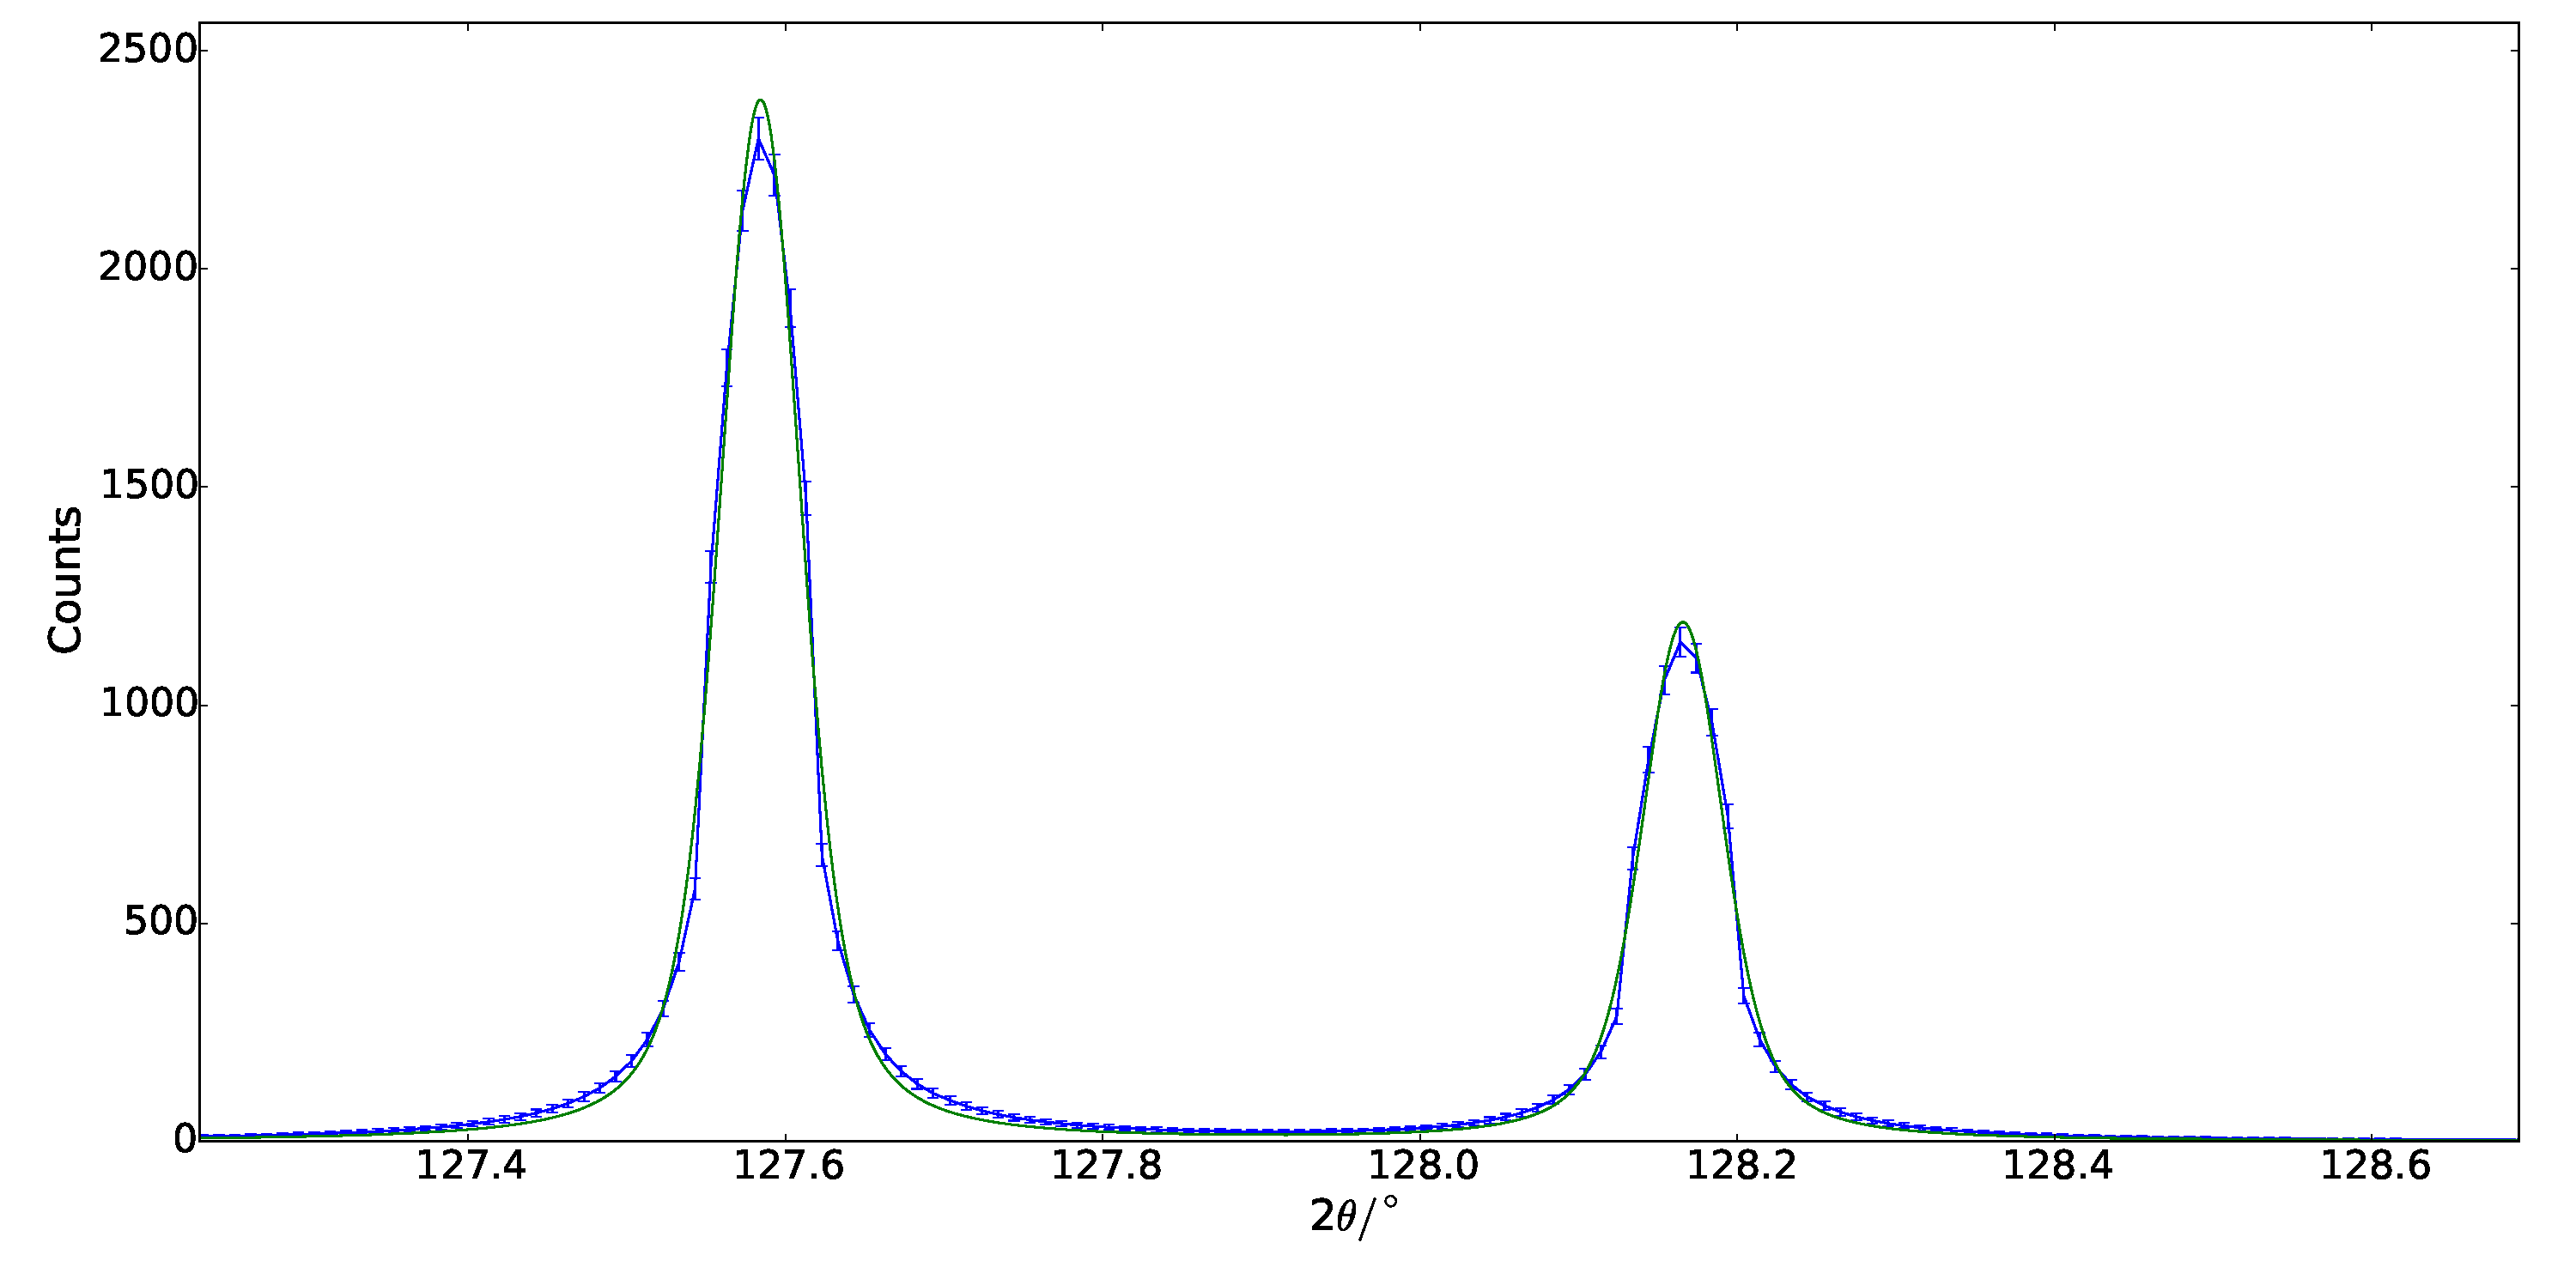
\includegraphics[scale=0.15]{messung_pulver_10}
  \captionof{figure}{Pulverdaten 10. Doppelpeak}
  \label{fig:pul_mess_10}
\end{minipage}
\end{figure}
\begin{figure}[H]
\begin{minipage}{.5\textwidth}
  \centering
  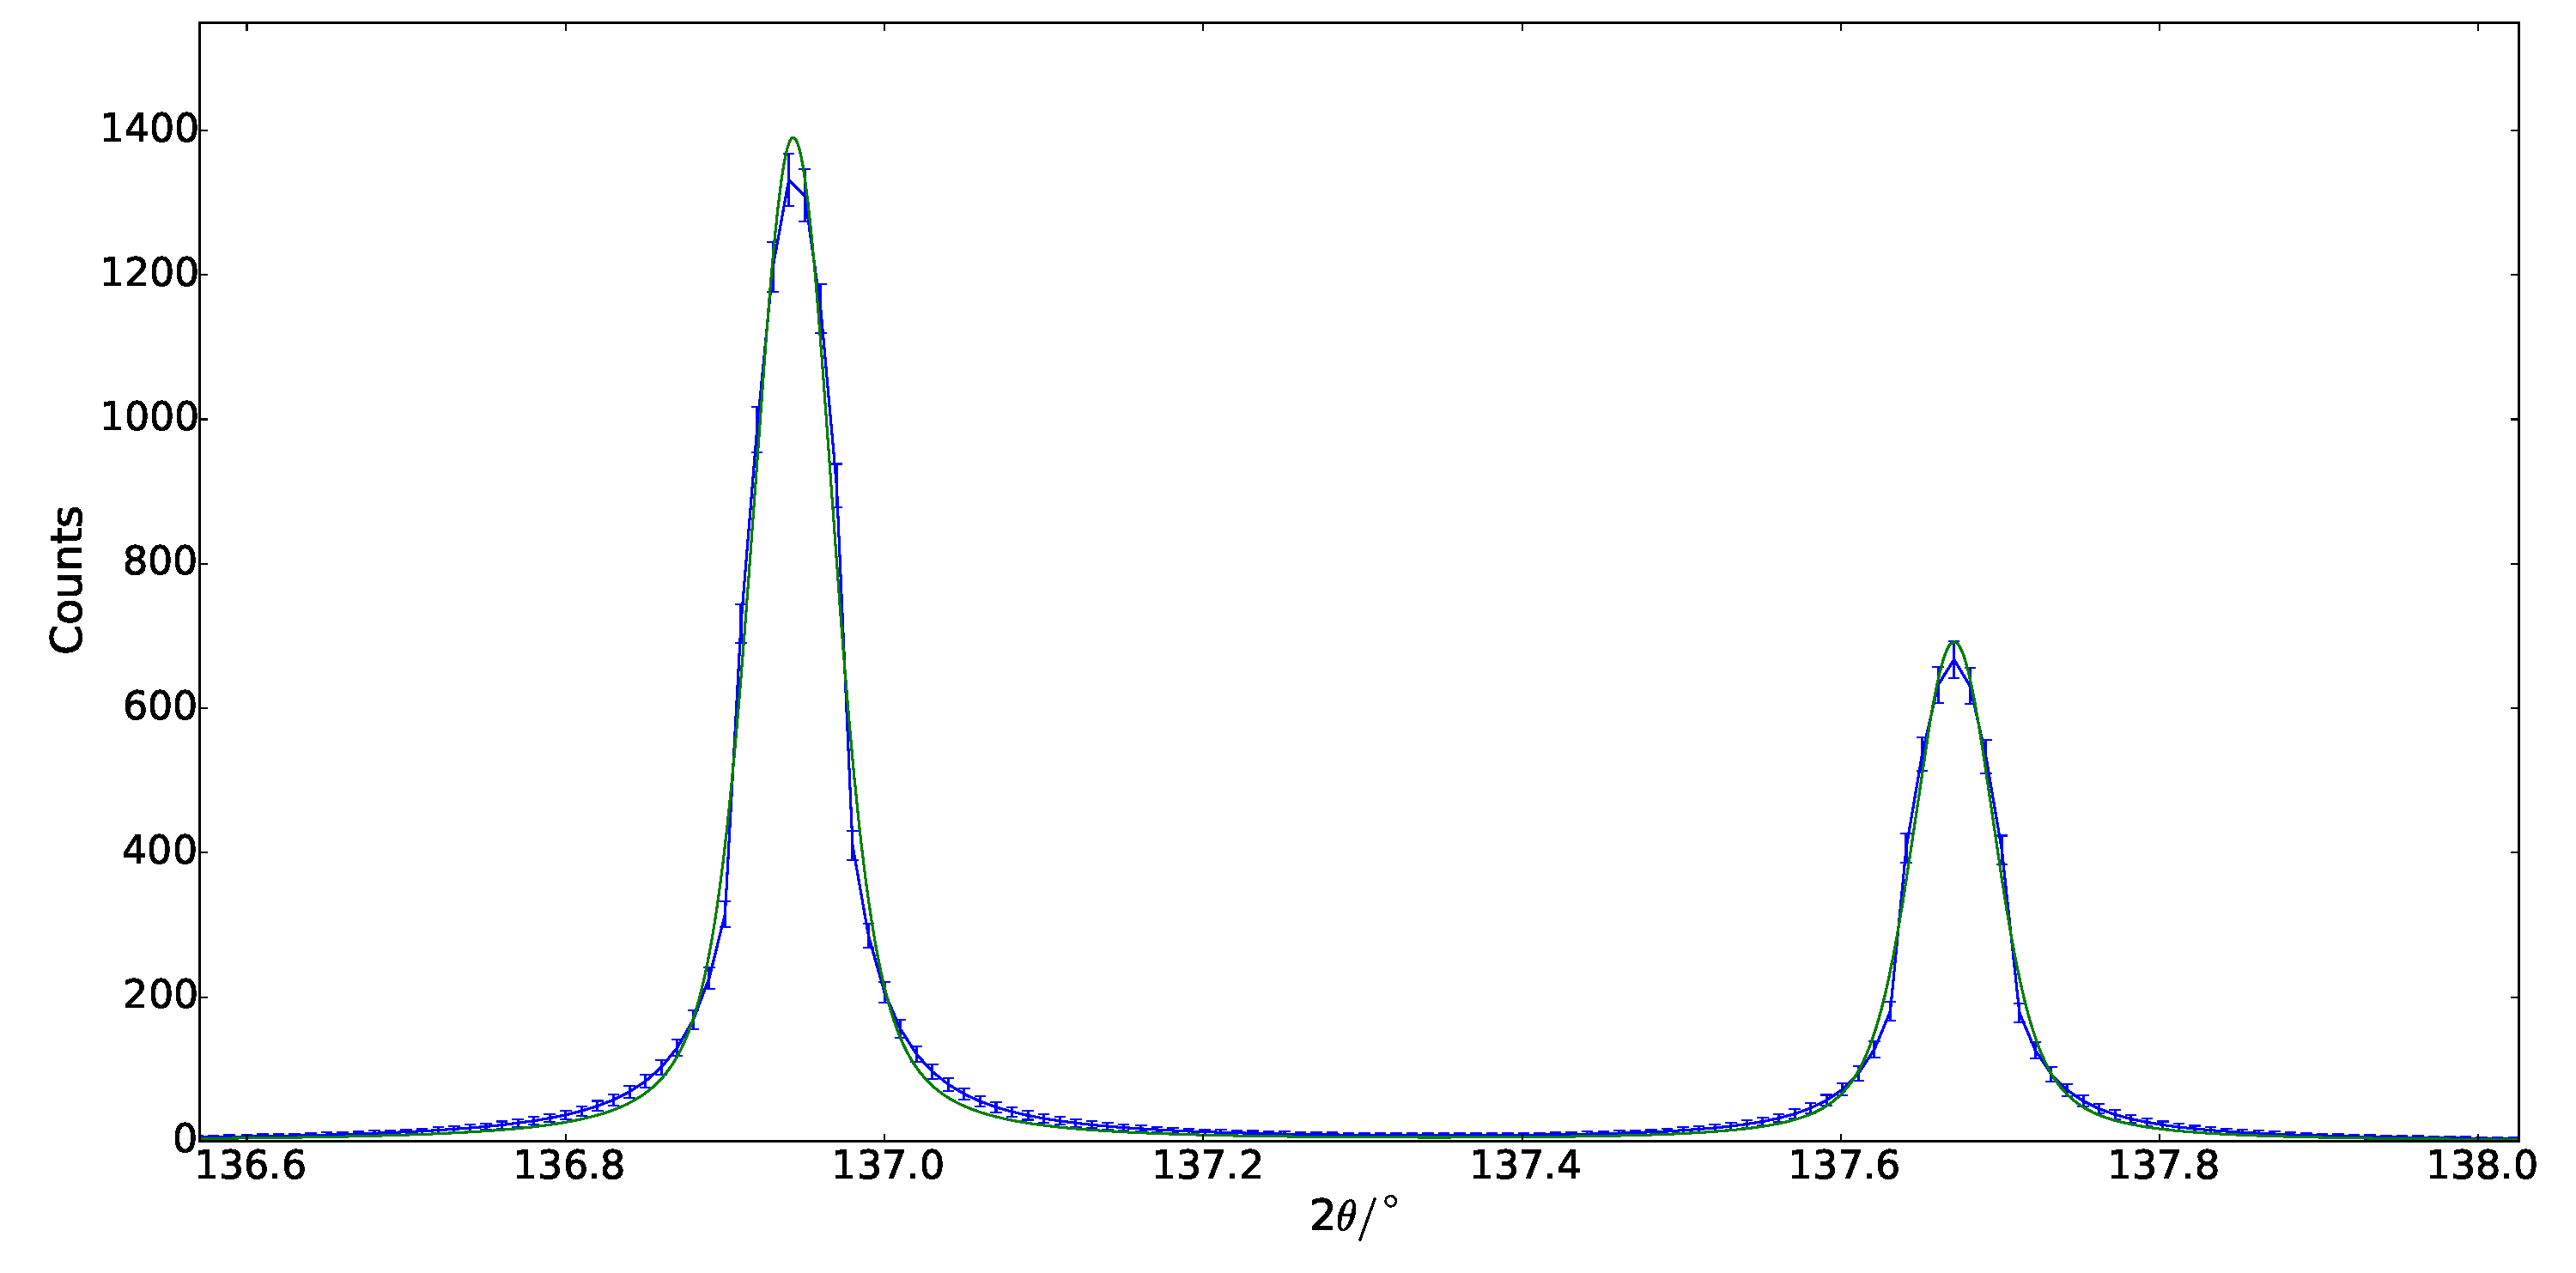
\includegraphics[scale=0.15]{messung_pulver_11}
  \captionof{figure}{Pulverdaten 11. Doppelpeak}
  \label{fig:pul_mess_11}
\end{minipage}
\end{figure}
Zum Vergleich sind die simulierten Peaks von Silicium
\begin{figure}[H]
\begin{minipage}{.5\textwidth}
  \centering
  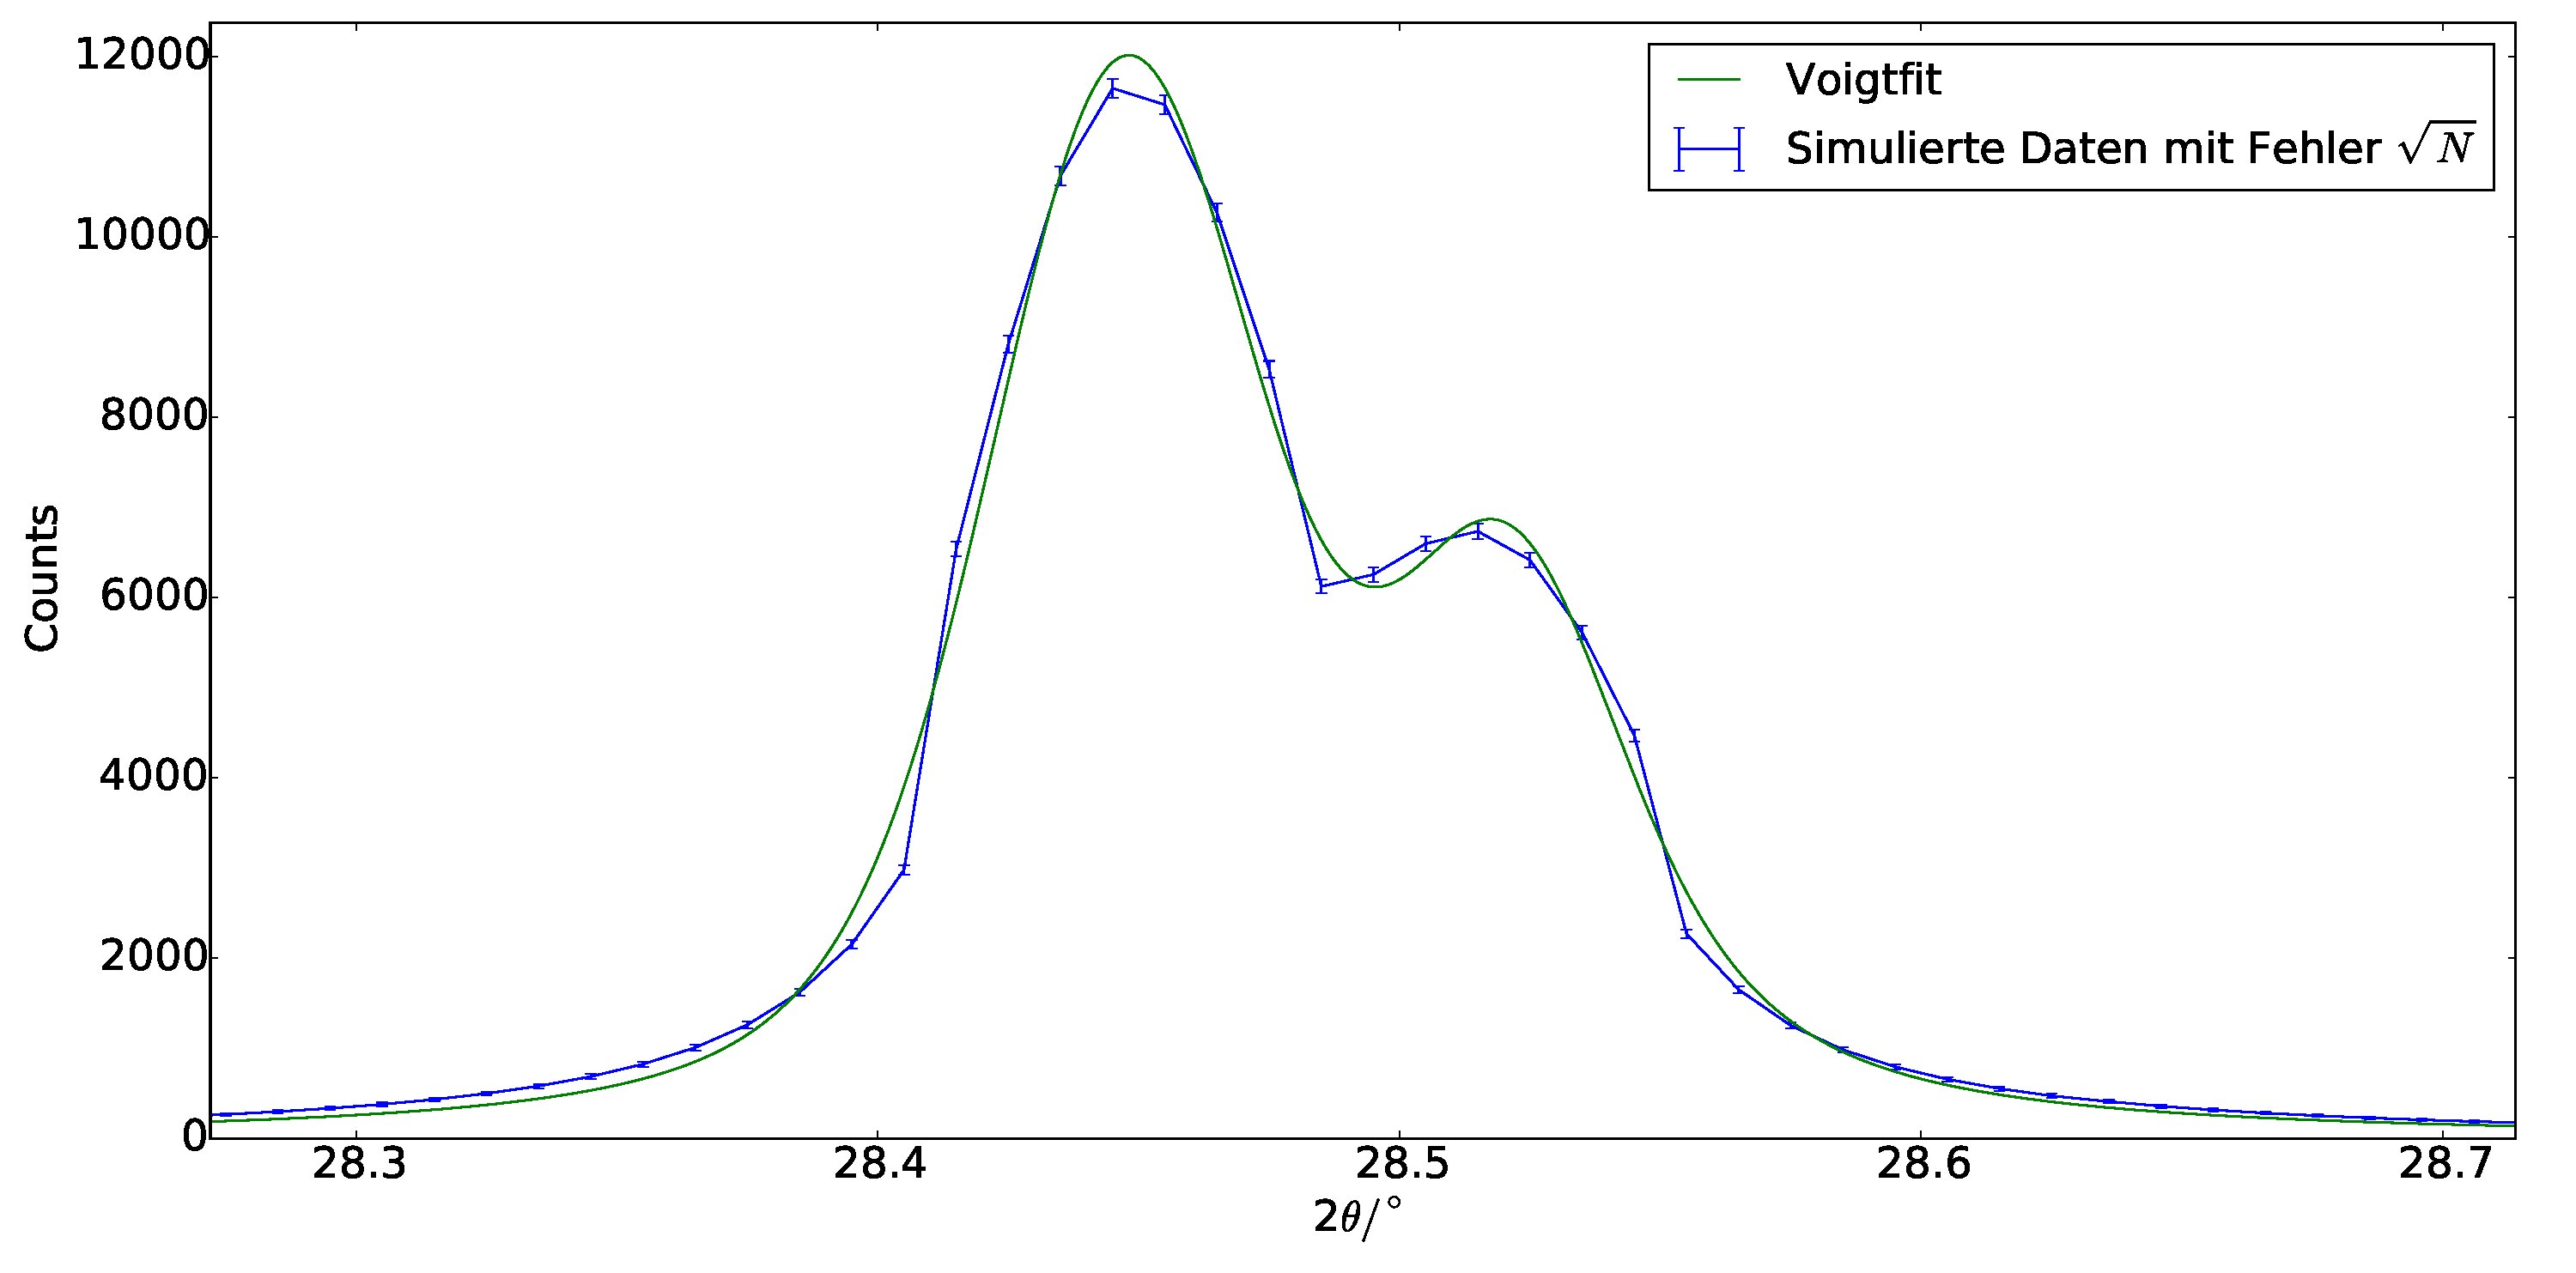
\includegraphics[scale=0.15]{Simulation_Siliciumpulver_1}
  \captionof{figure}{Siliciumpulver 1. Doppelpeak}
  \label{fig:pul_sim_sil_1}
\end{minipage}
\hspace{0.5cm}
\begin{minipage}{.5\textwidth}
  \centering
  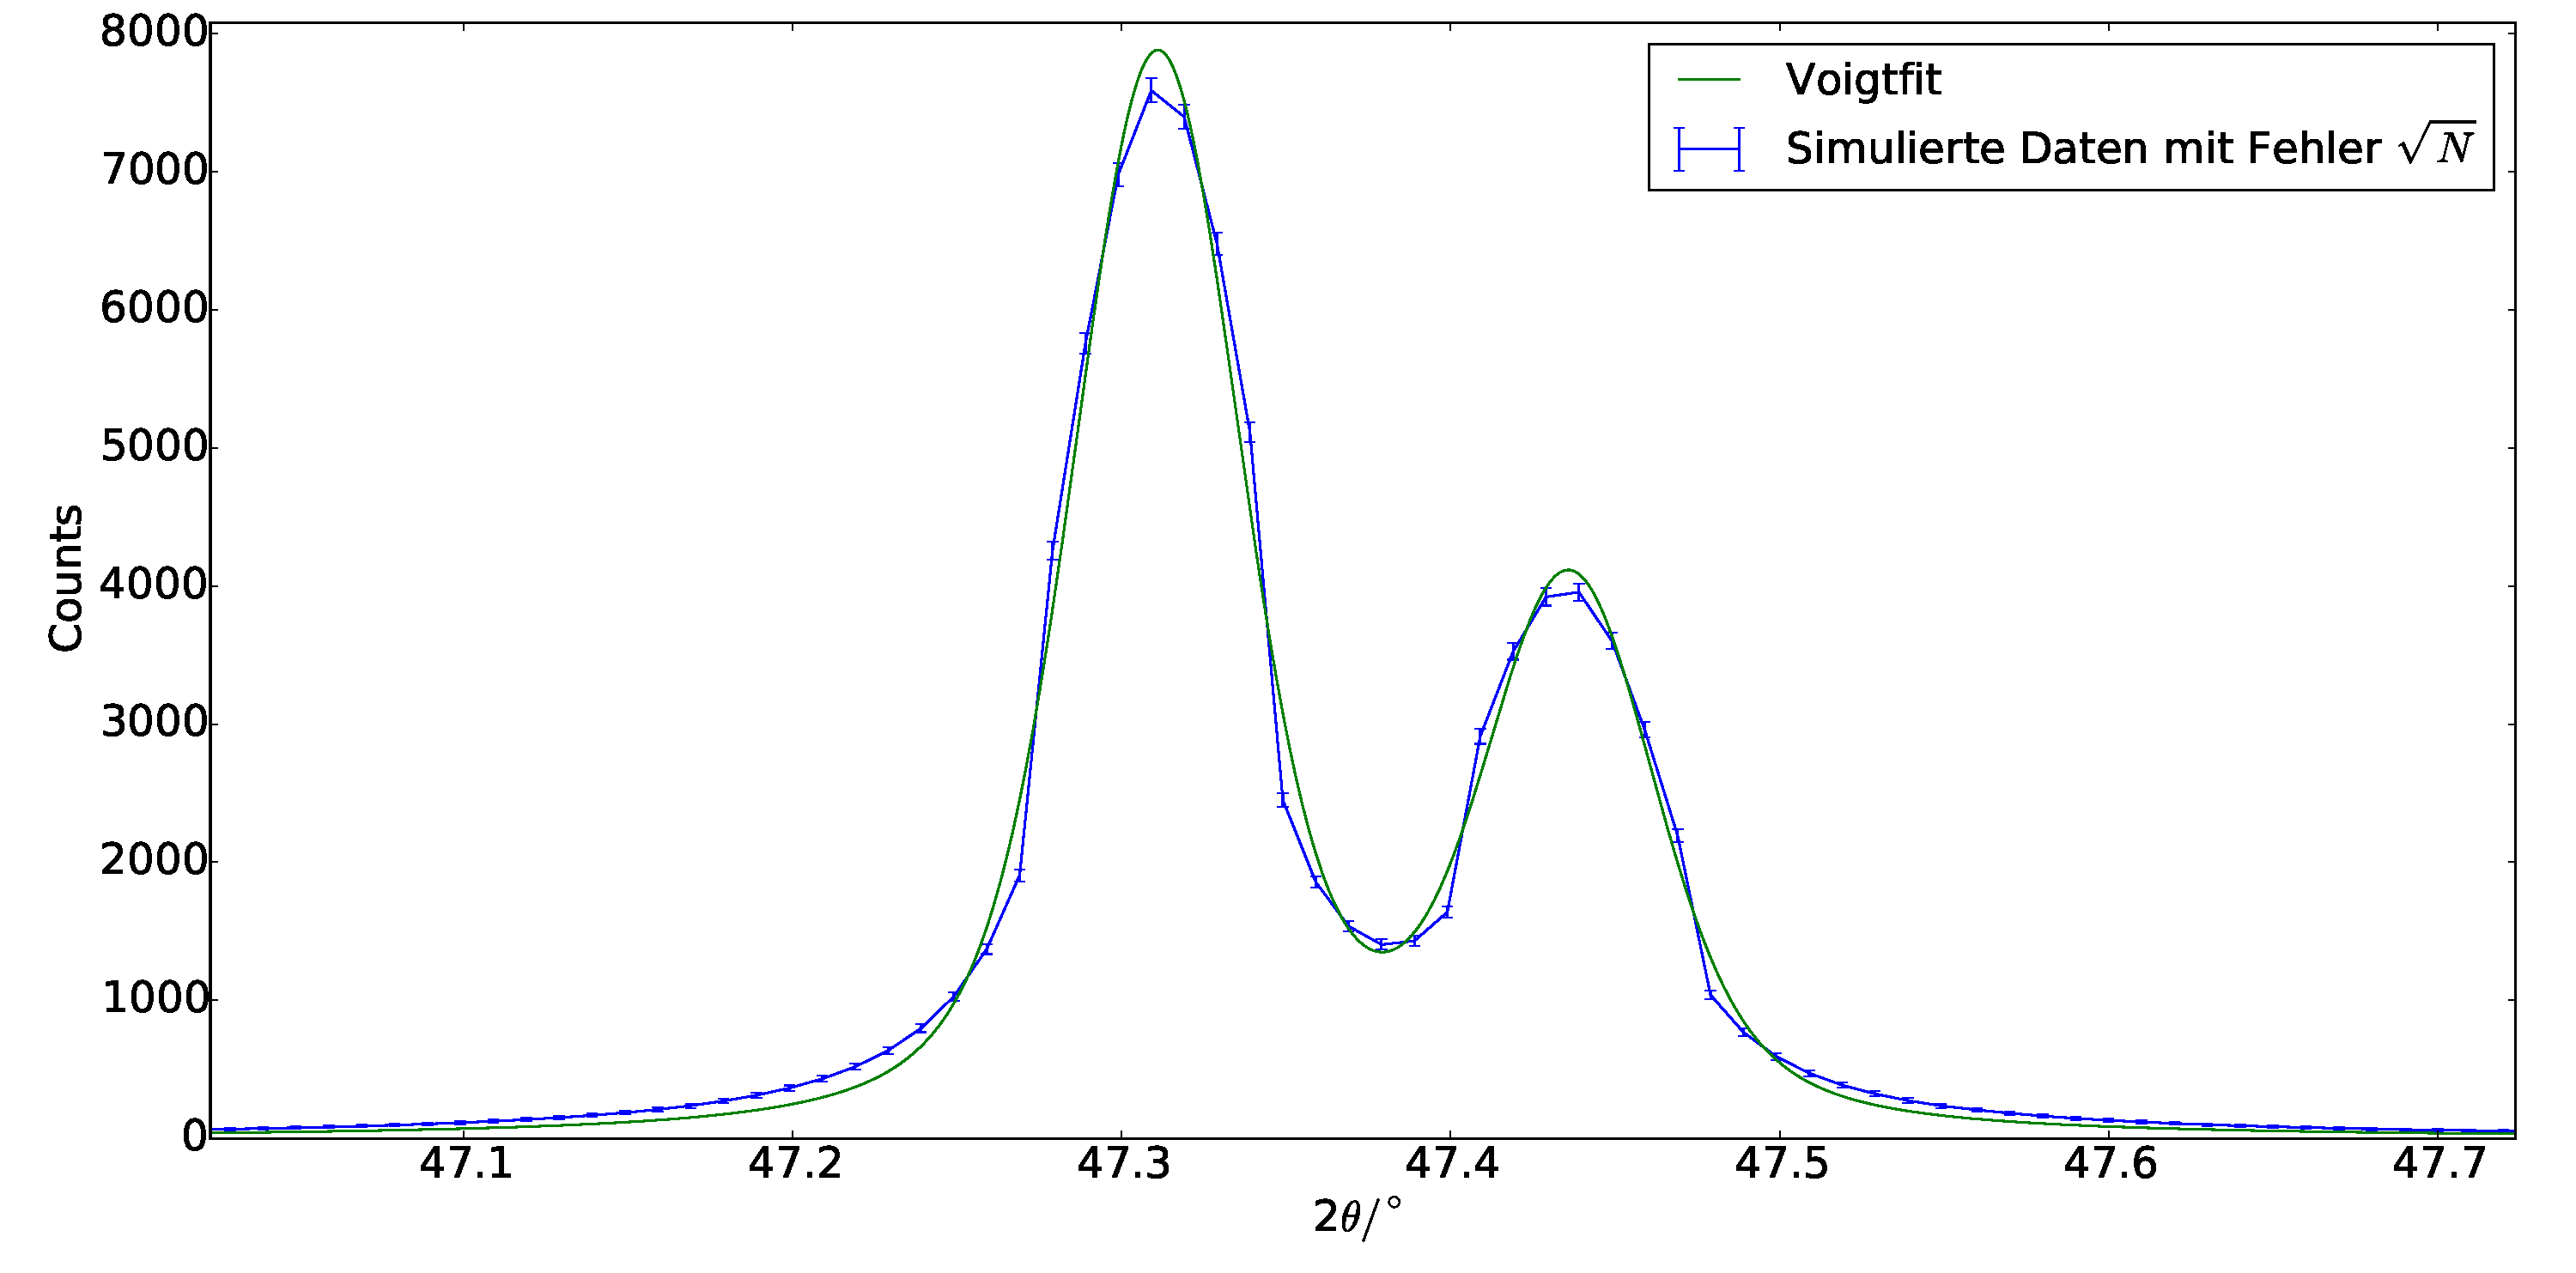
\includegraphics[scale=0.15]{Simulation_Siliciumpulver_2}
  \captionof{figure}{Siliciumpulver 2. Doppelpeak}
  \label{fig:pul_sim_sil_2}
\end{minipage}
\end{figure}
\begin{figure}[H]
\begin{minipage}{.5\textwidth}
  \centering
  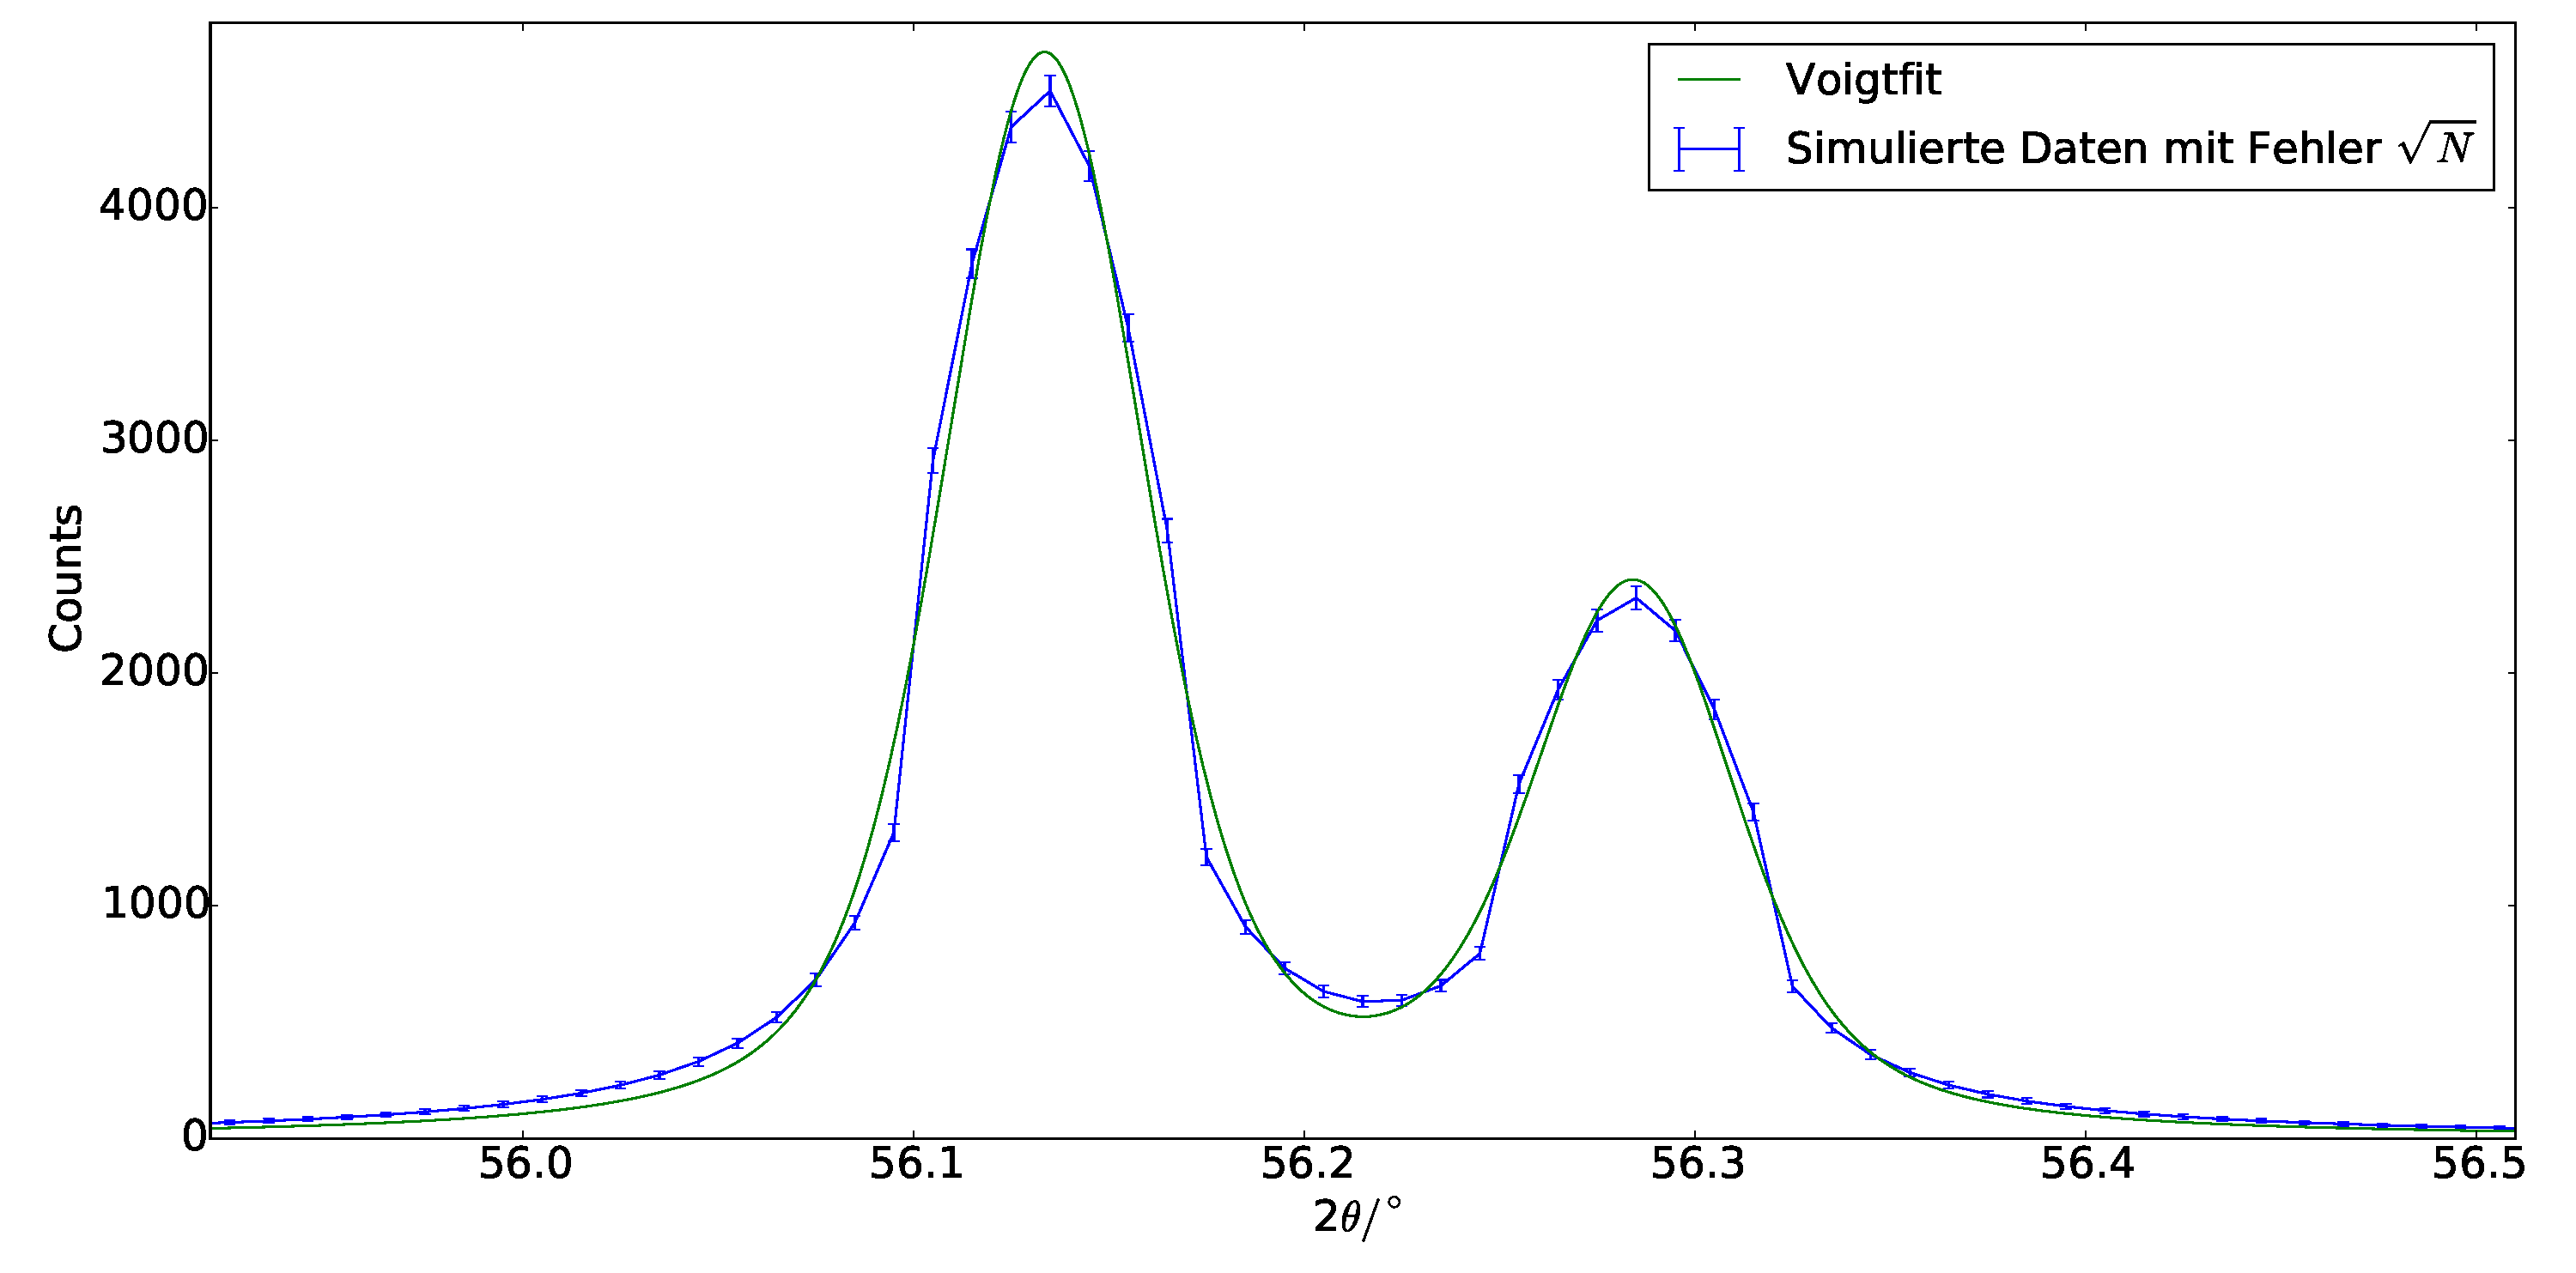
\includegraphics[scale=0.15]{Simulation_Siliciumpulver_3}
  \captionof{figure}{Siliciumpulver 3. Doppelpeak}
  \label{fig:pul_sim_sil_3}
\end{minipage}
\hspace{0.5cm}
\begin{minipage}{.5\textwidth}
  \centering
  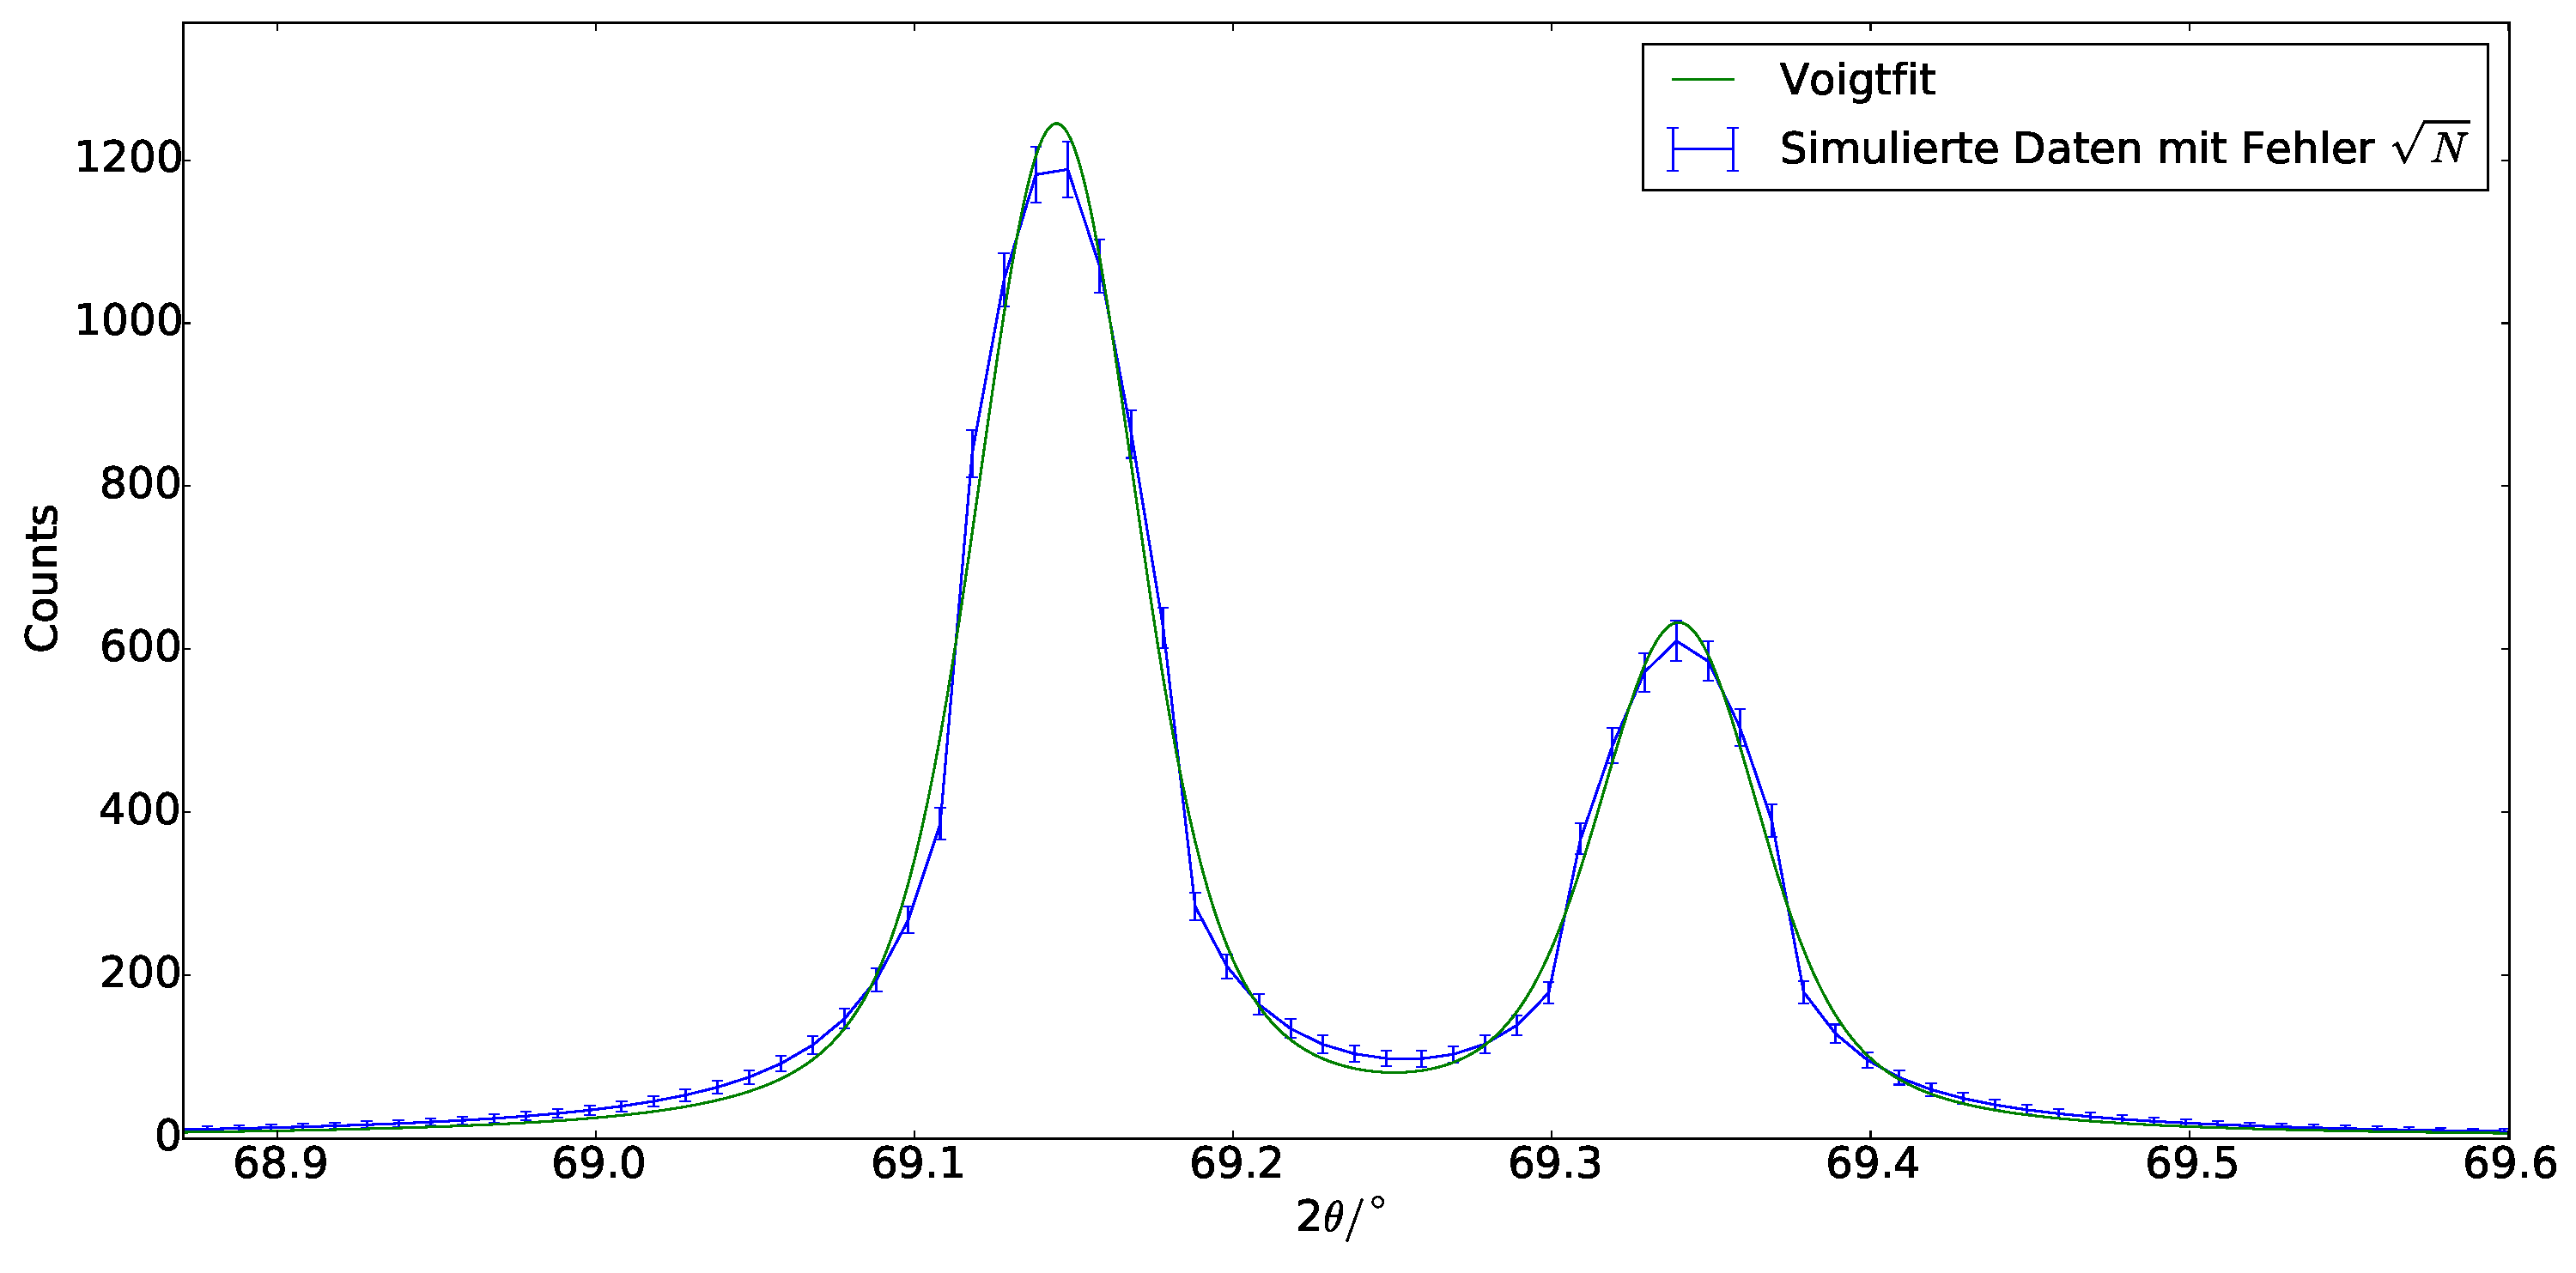
\includegraphics[scale=0.15]{Simulation_Siliciumpulver_4}
  \captionof{figure}{Siliciumpulver 4. Doppelpeak}
  \label{fig:pul_sim_sil_4}
\end{minipage}
\end{figure}
\begin{figure}[H]
\begin{minipage}{.5\textwidth}
  \centering
  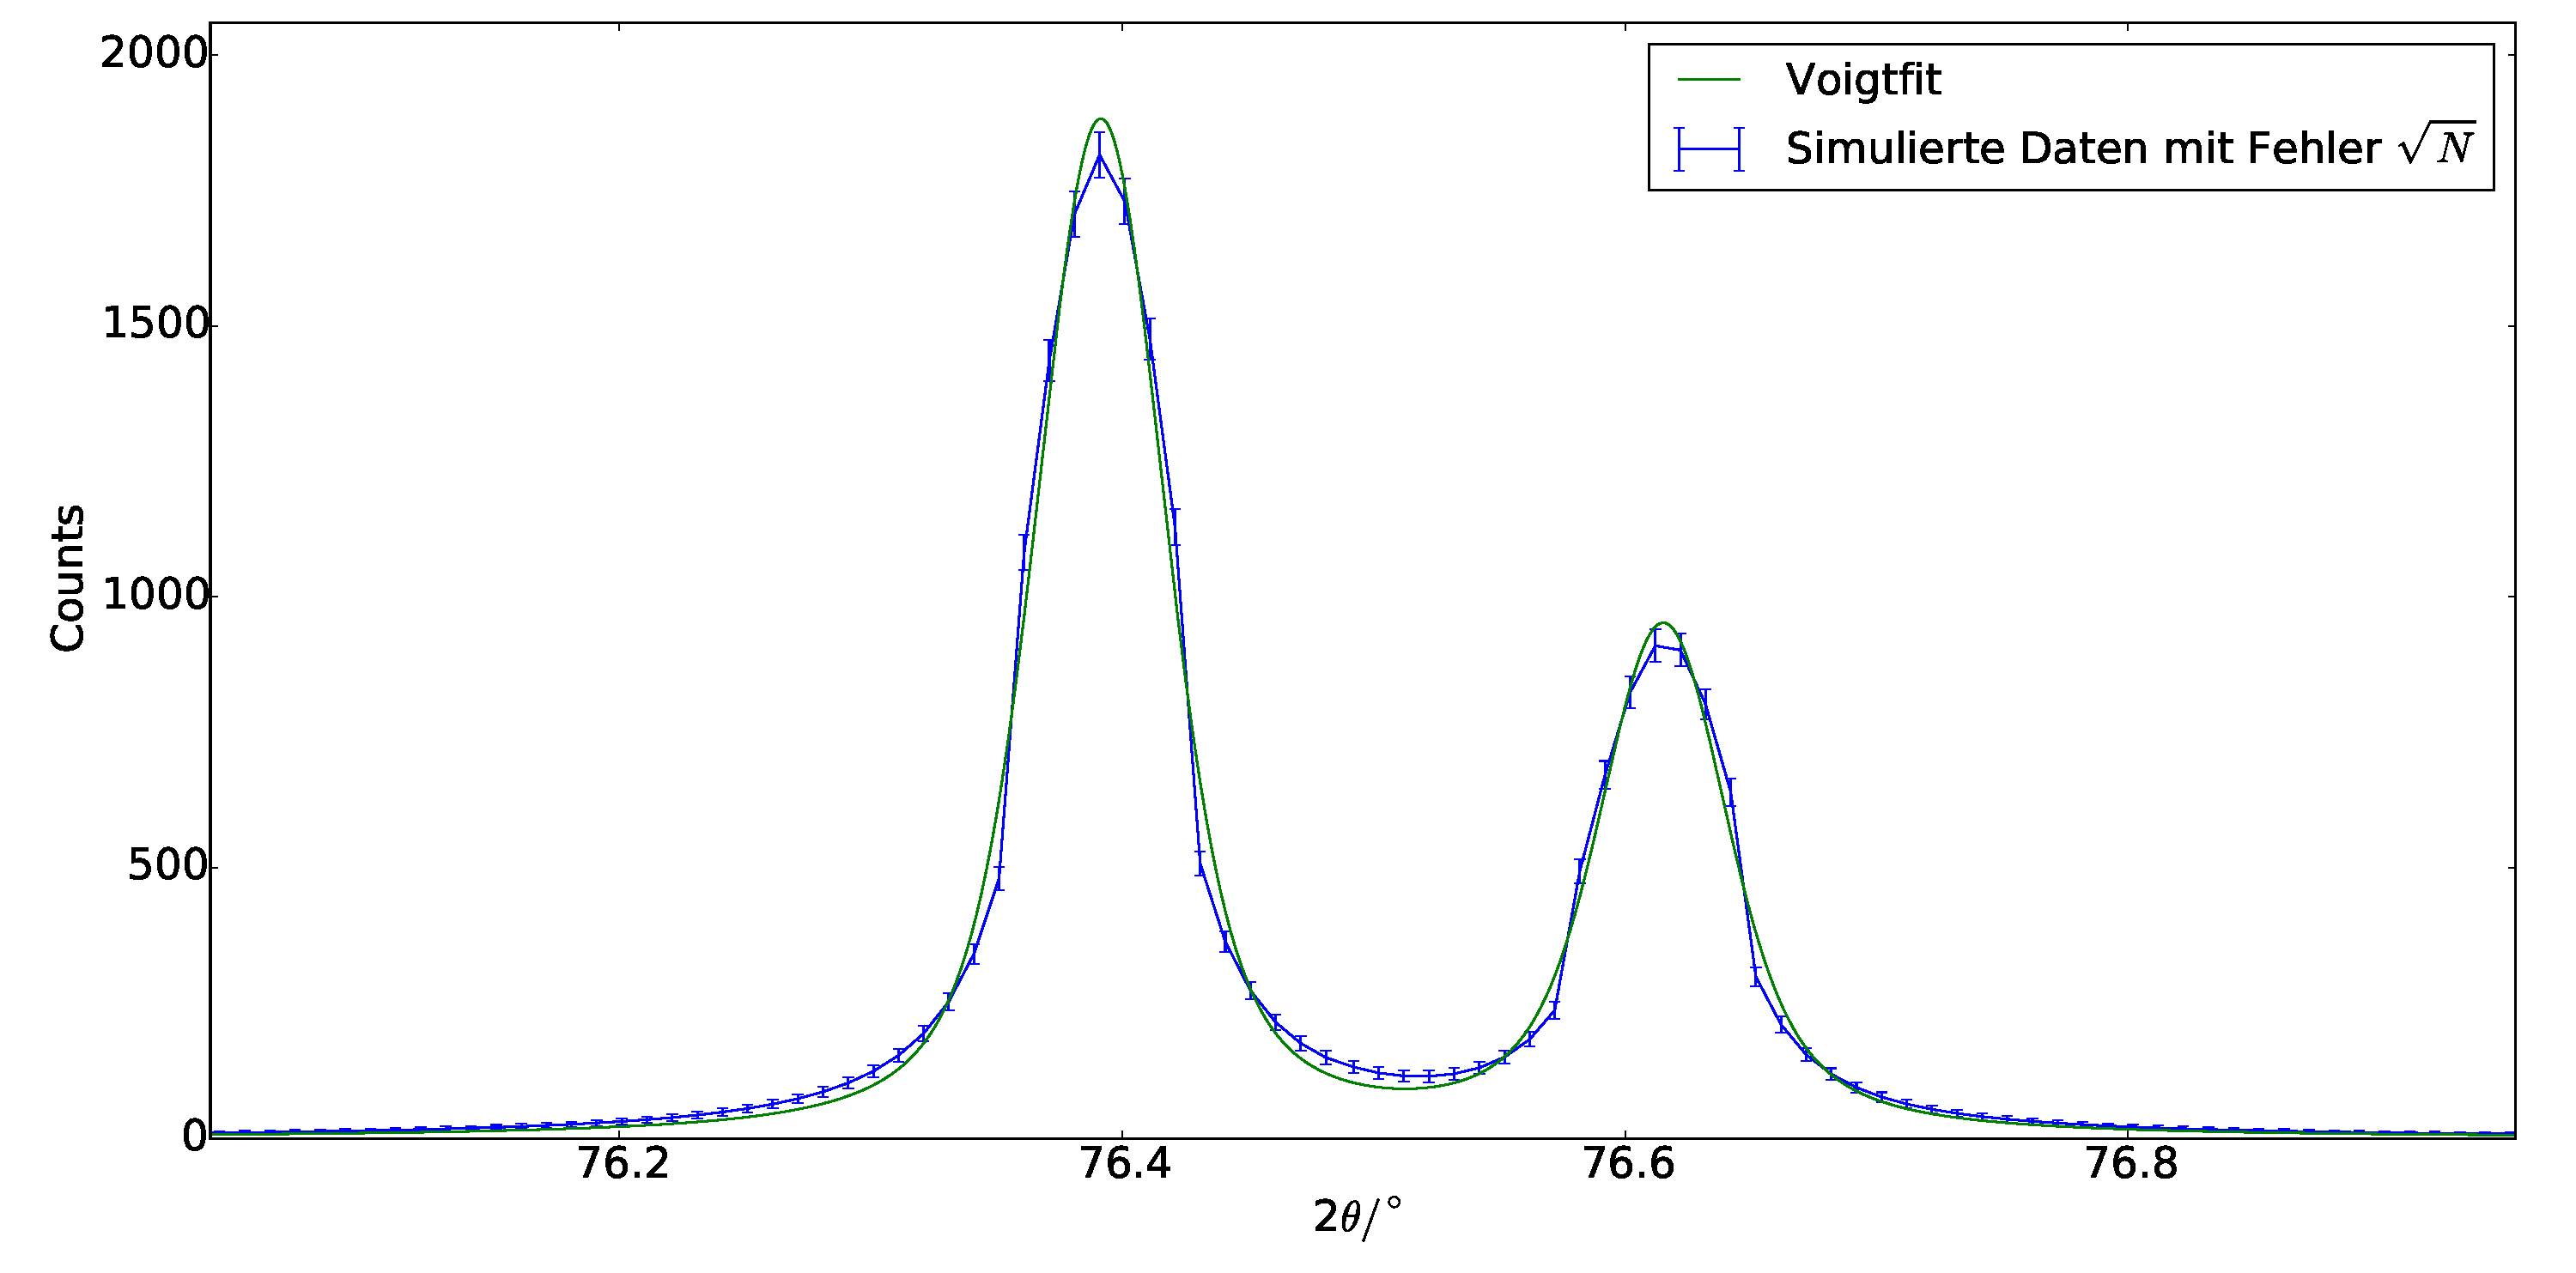
\includegraphics[scale=0.15]{Simulation_Siliciumpulver_5}
  \captionof{figure}{Siliciumpulver 5. Doppelpeak}
  \label{fig:pul_sim_sil_5}
\end{minipage}
\hspace{0.5cm}
\begin{minipage}{.5\textwidth}
  \centering
  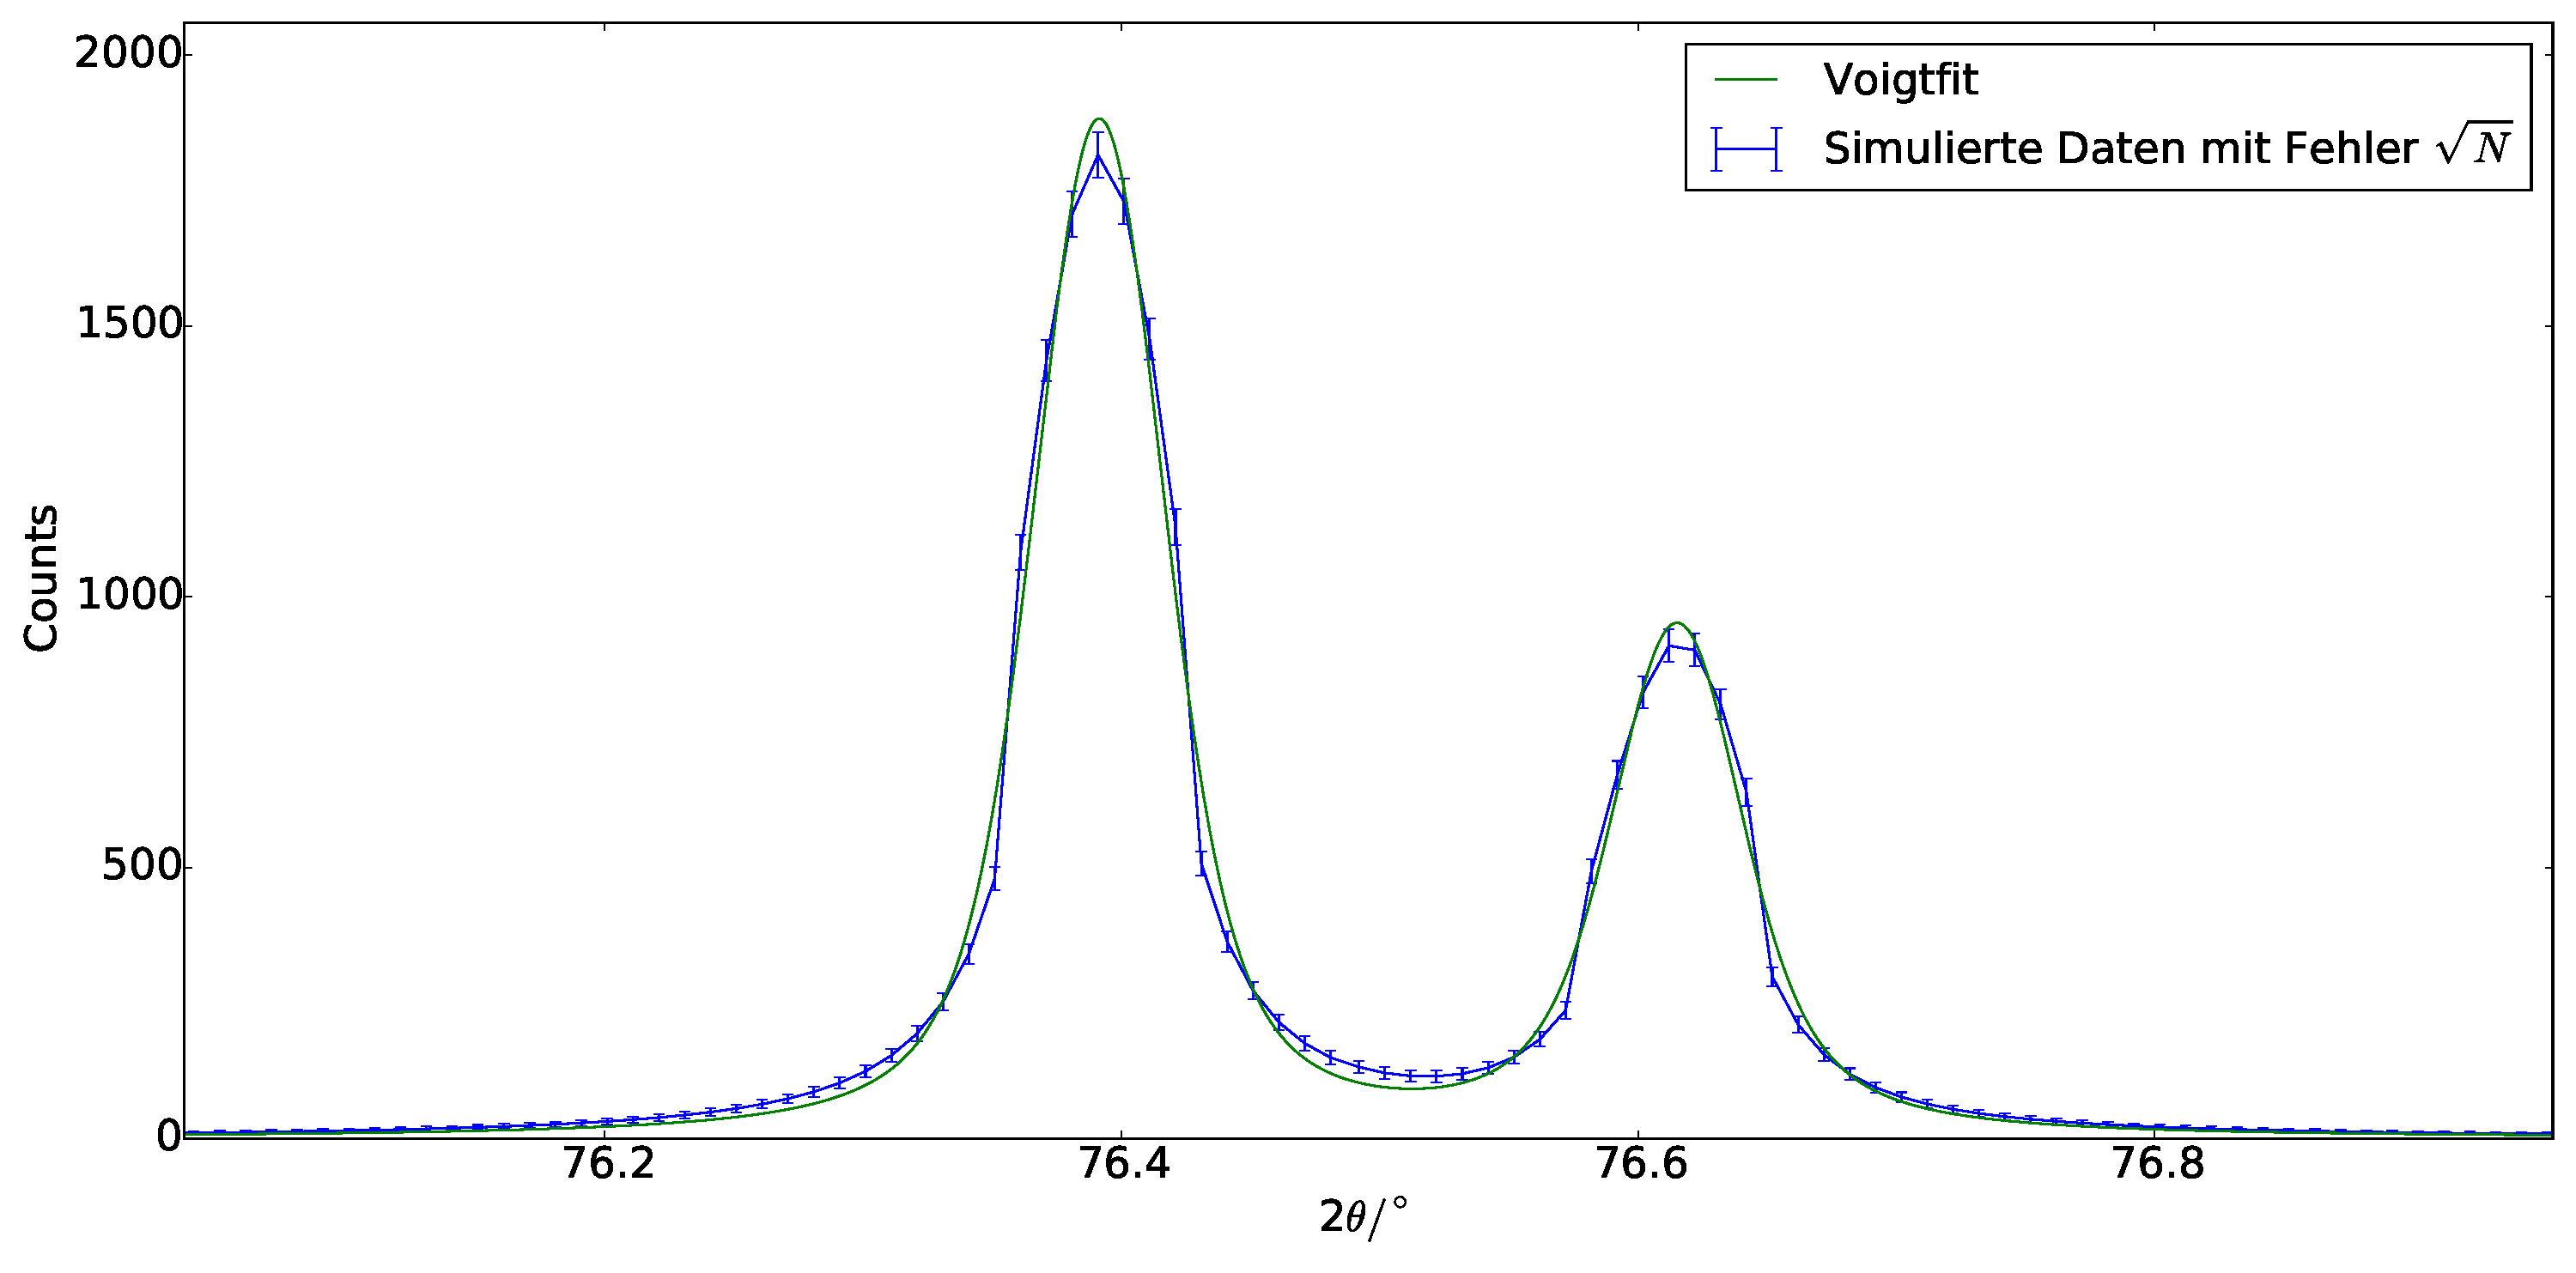
\includegraphics[scale=0.15]{Simulation_Siliciumpulver_6}
  \captionof{figure}{Siliciumpulver 6. Doppelpeak}
  \label{fig:pul_sim_sil_6}
\end{minipage}
\end{figure}
\begin{figure}[H]
\begin{minipage}{.5\textwidth}
  \centering
  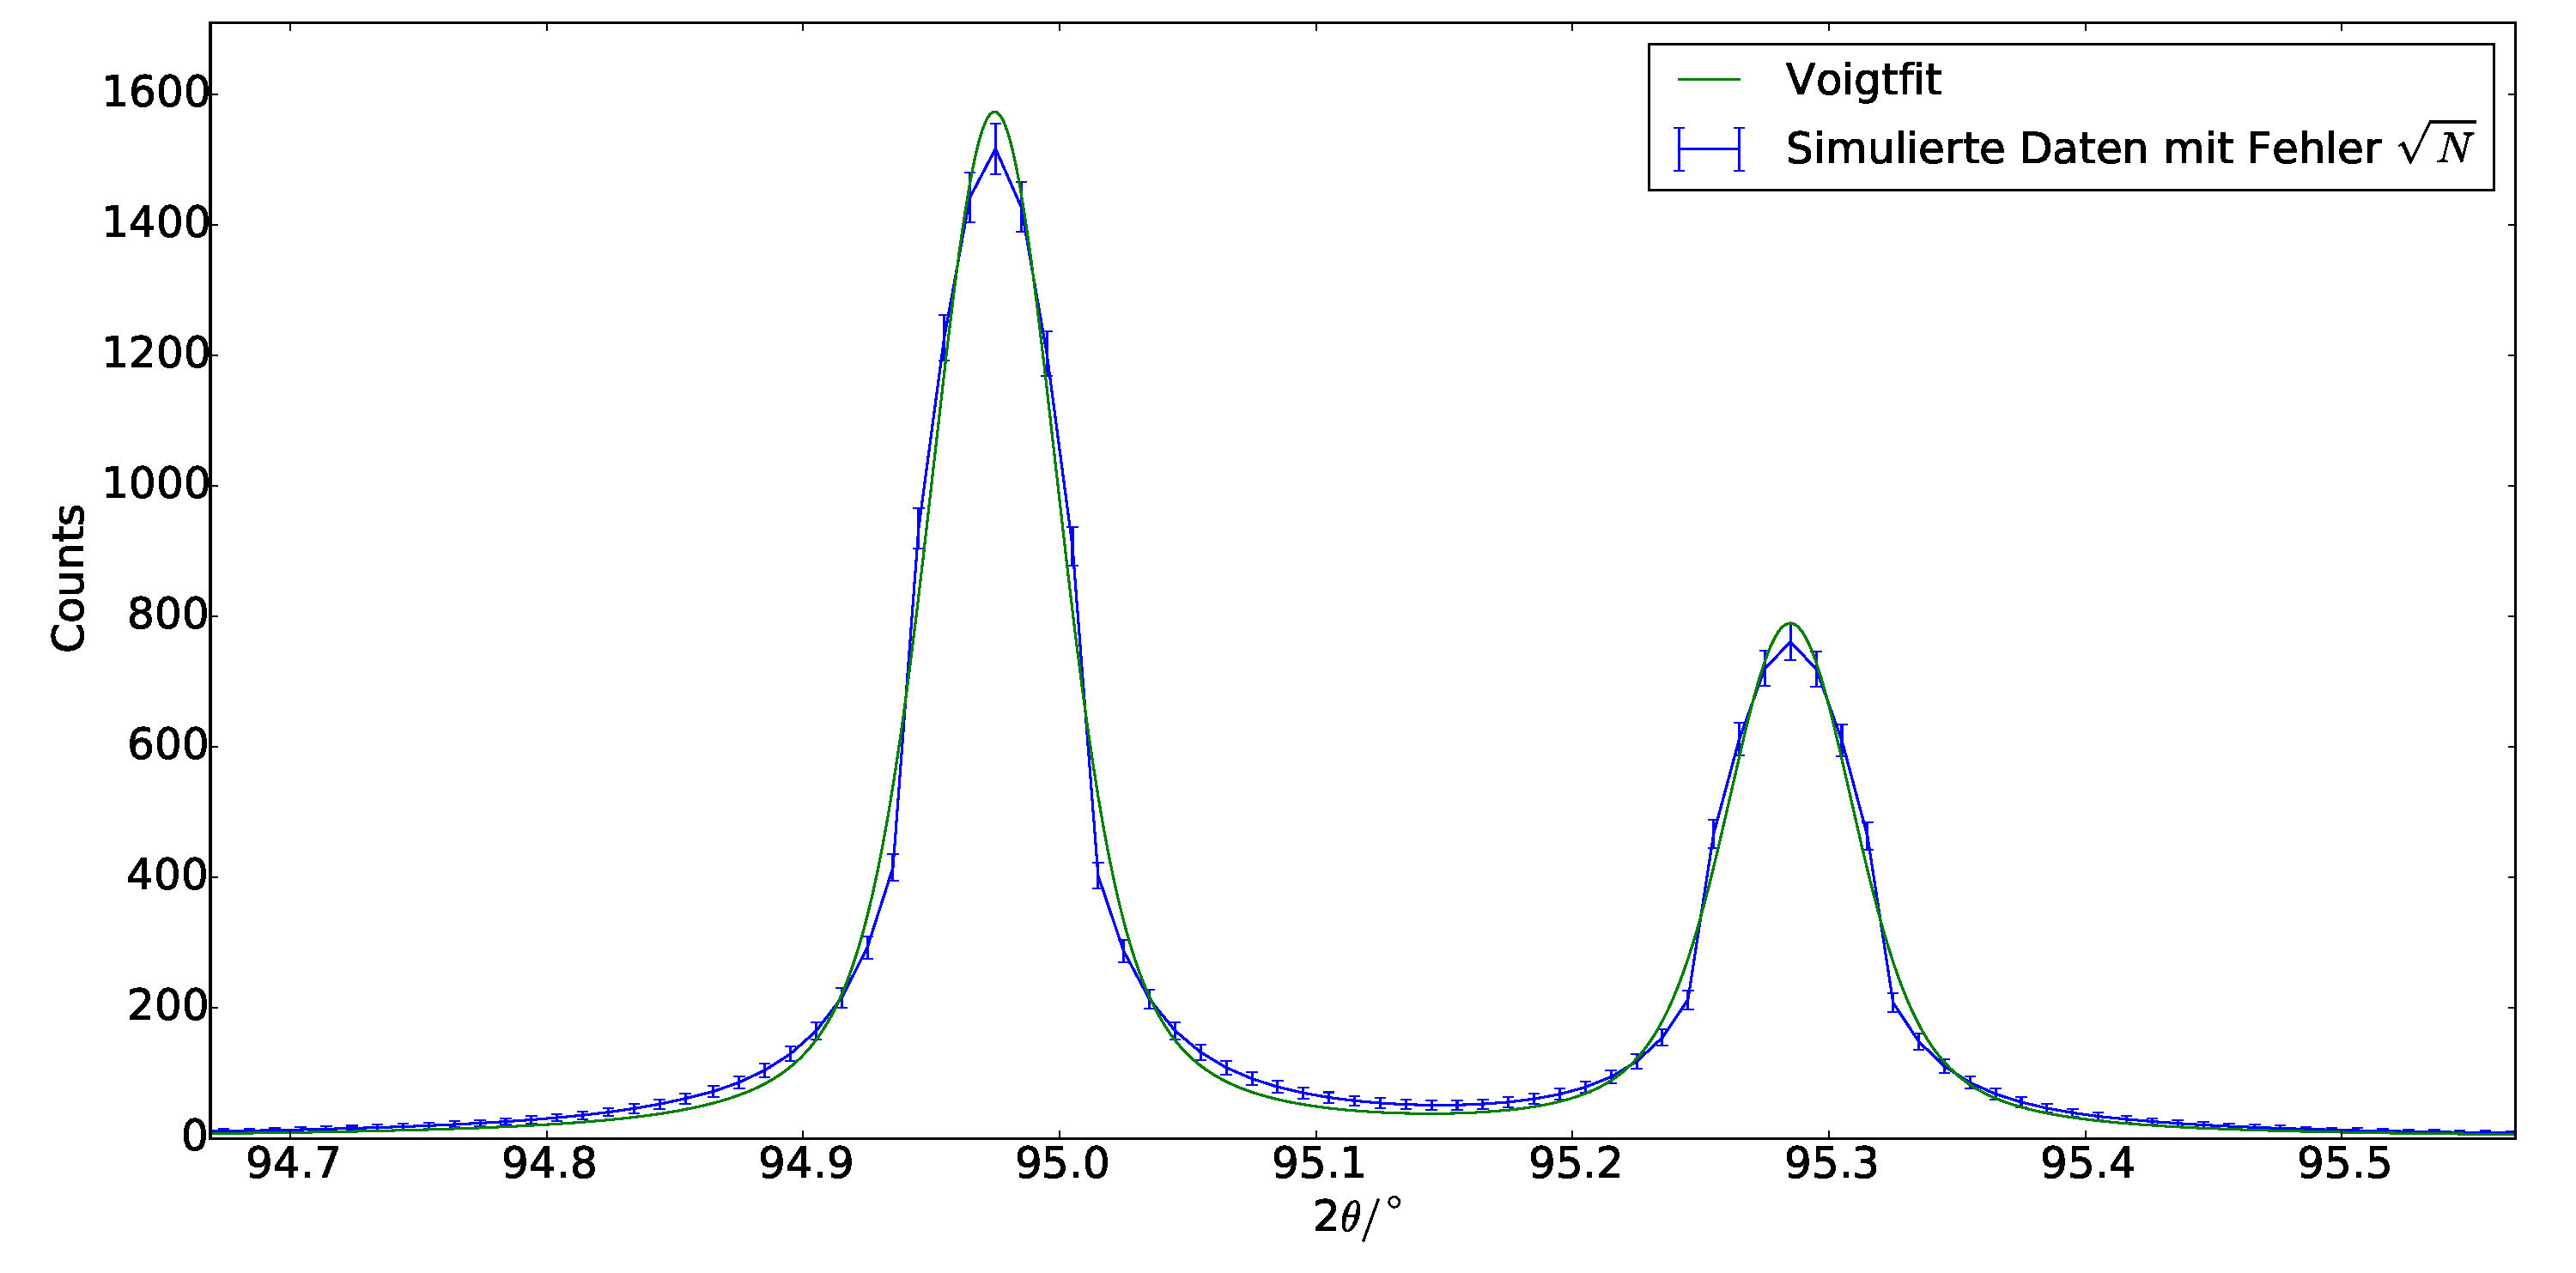
\includegraphics[scale=0.15]{Simulation_Siliciumpulver_7}
  \captionof{figure}{Siliciumpulver 7. Doppelpeak}
  \label{fig:pul_sim_sil_7}
\end{minipage}
\hspace{0.5cm}
\begin{minipage}{.5\textwidth}
  \centering
  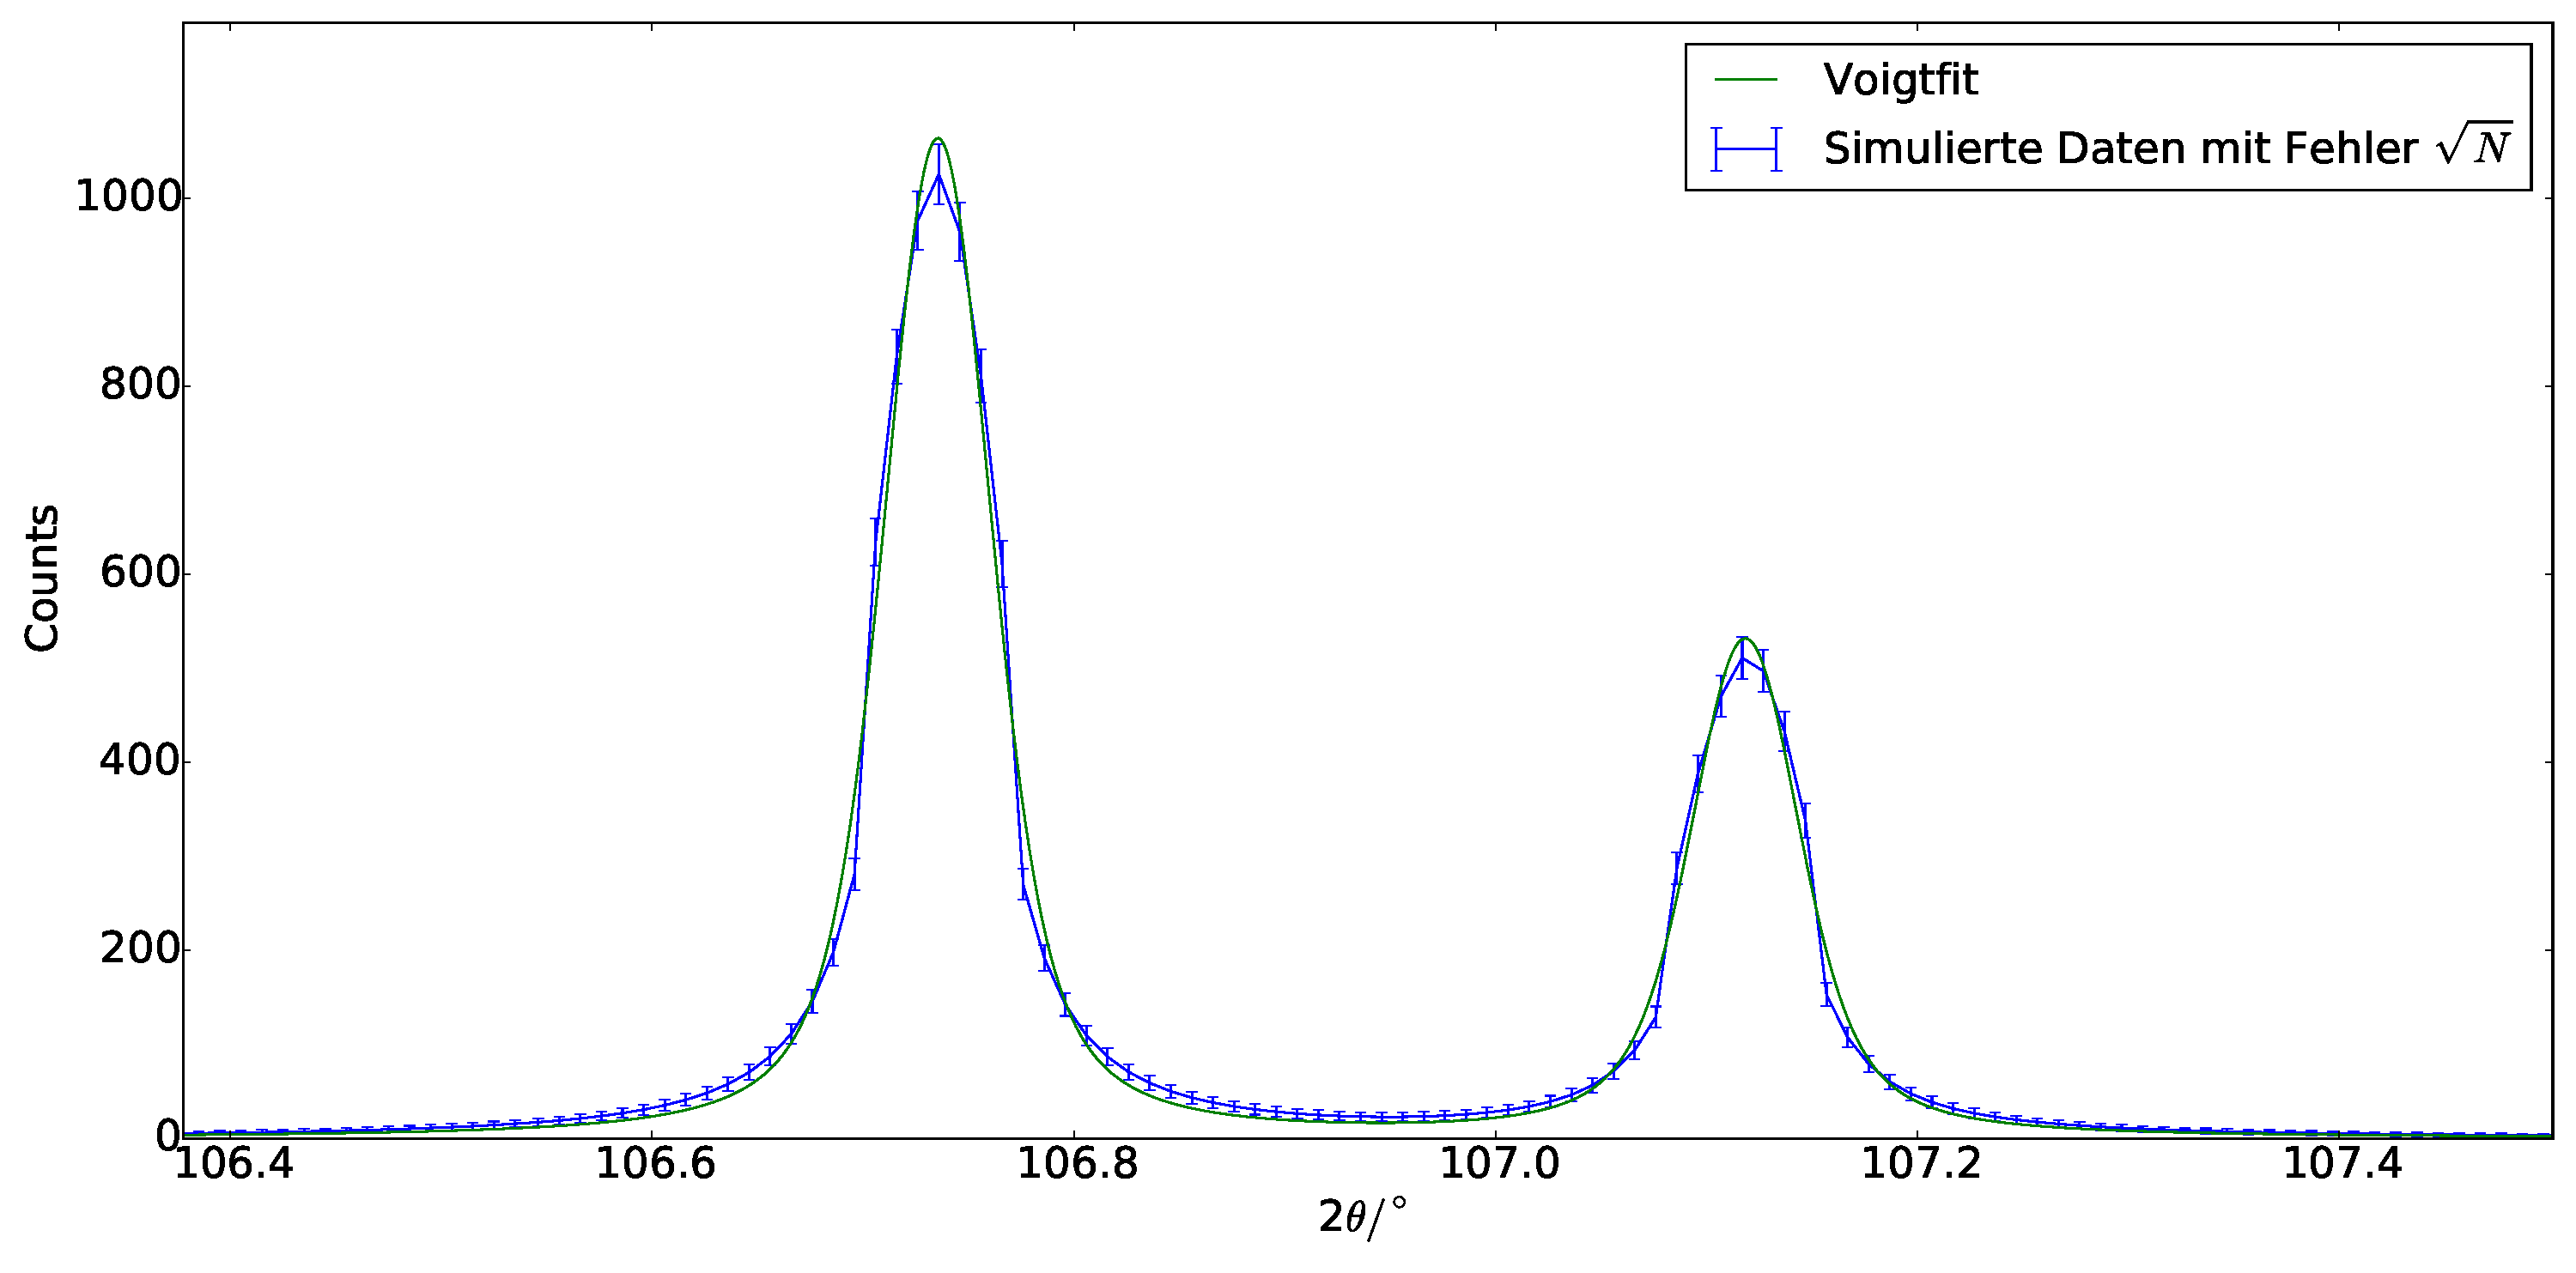
\includegraphics[scale=0.15]{Simulation_Siliciumpulver_8}
  \captionof{figure}{Siliciumpulver 8. Doppelpeak}
  \label{fig:pul_sim_sil_8}
\end{minipage}
\end{figure}
\begin{figure}[H]
\begin{minipage}{.5\textwidth}
  \centering
  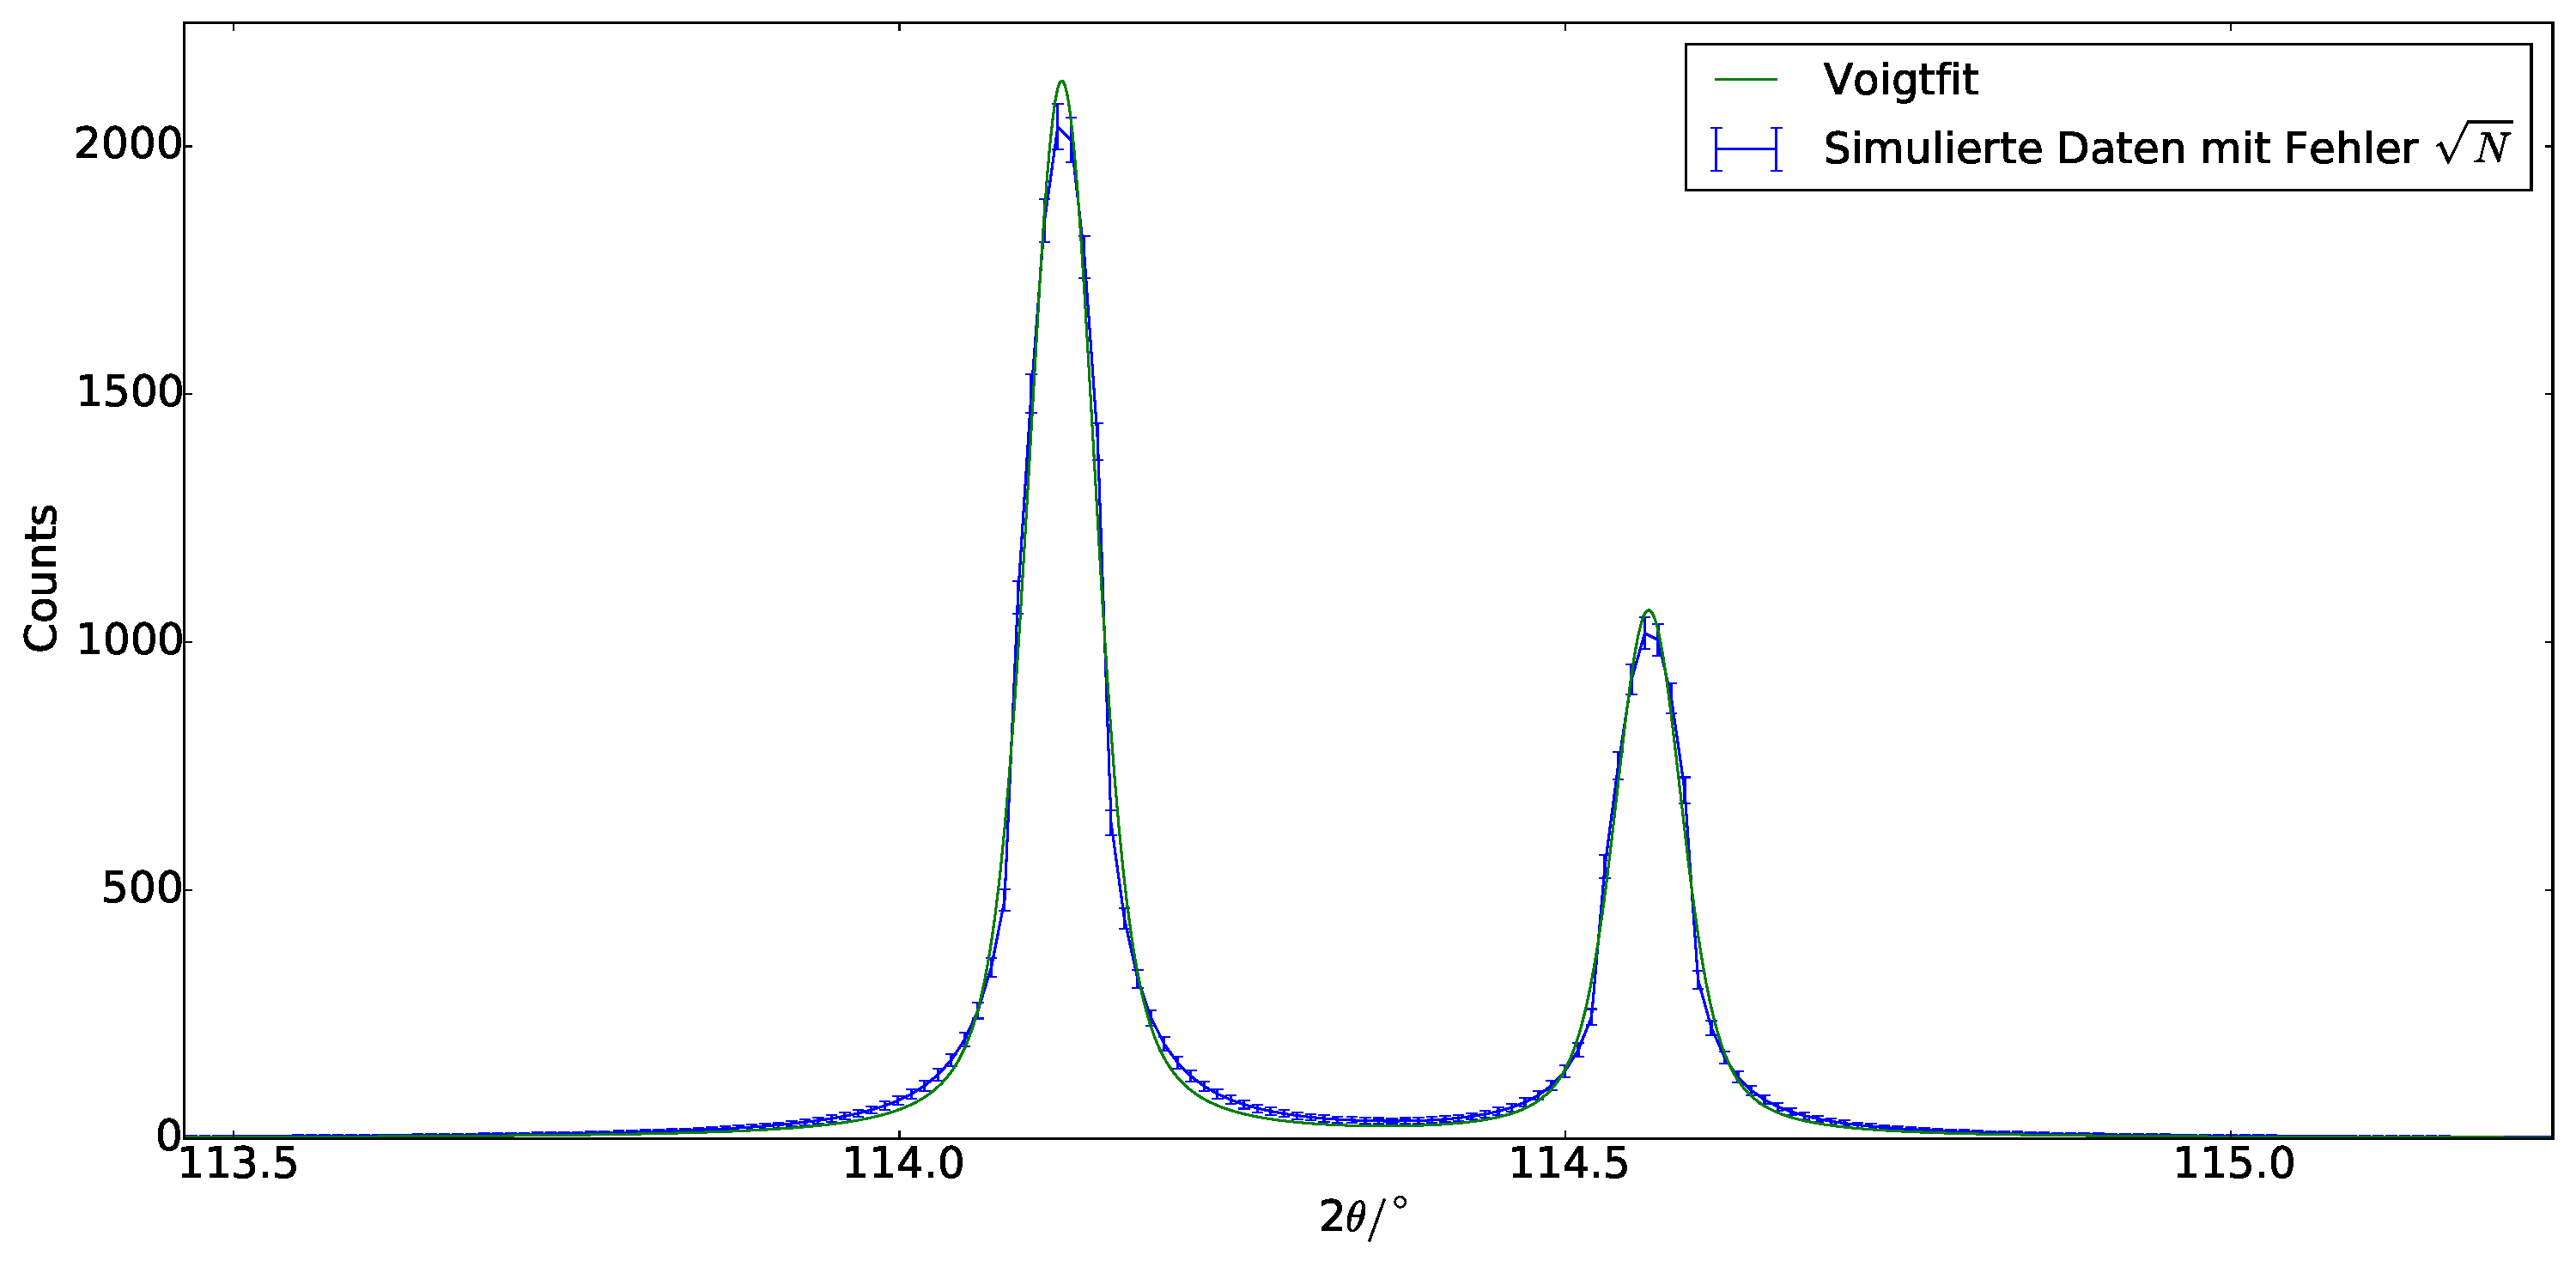
\includegraphics[scale=0.15]{Simulation_Siliciumpulver_9}
  \captionof{figure}{Siliciumpulver 9. Doppelpeak}
  \label{fig:pul_sim_sil_9}
\end{minipage}
\hspace{0.5cm}
\begin{minipage}{.5\textwidth}
  \centering
  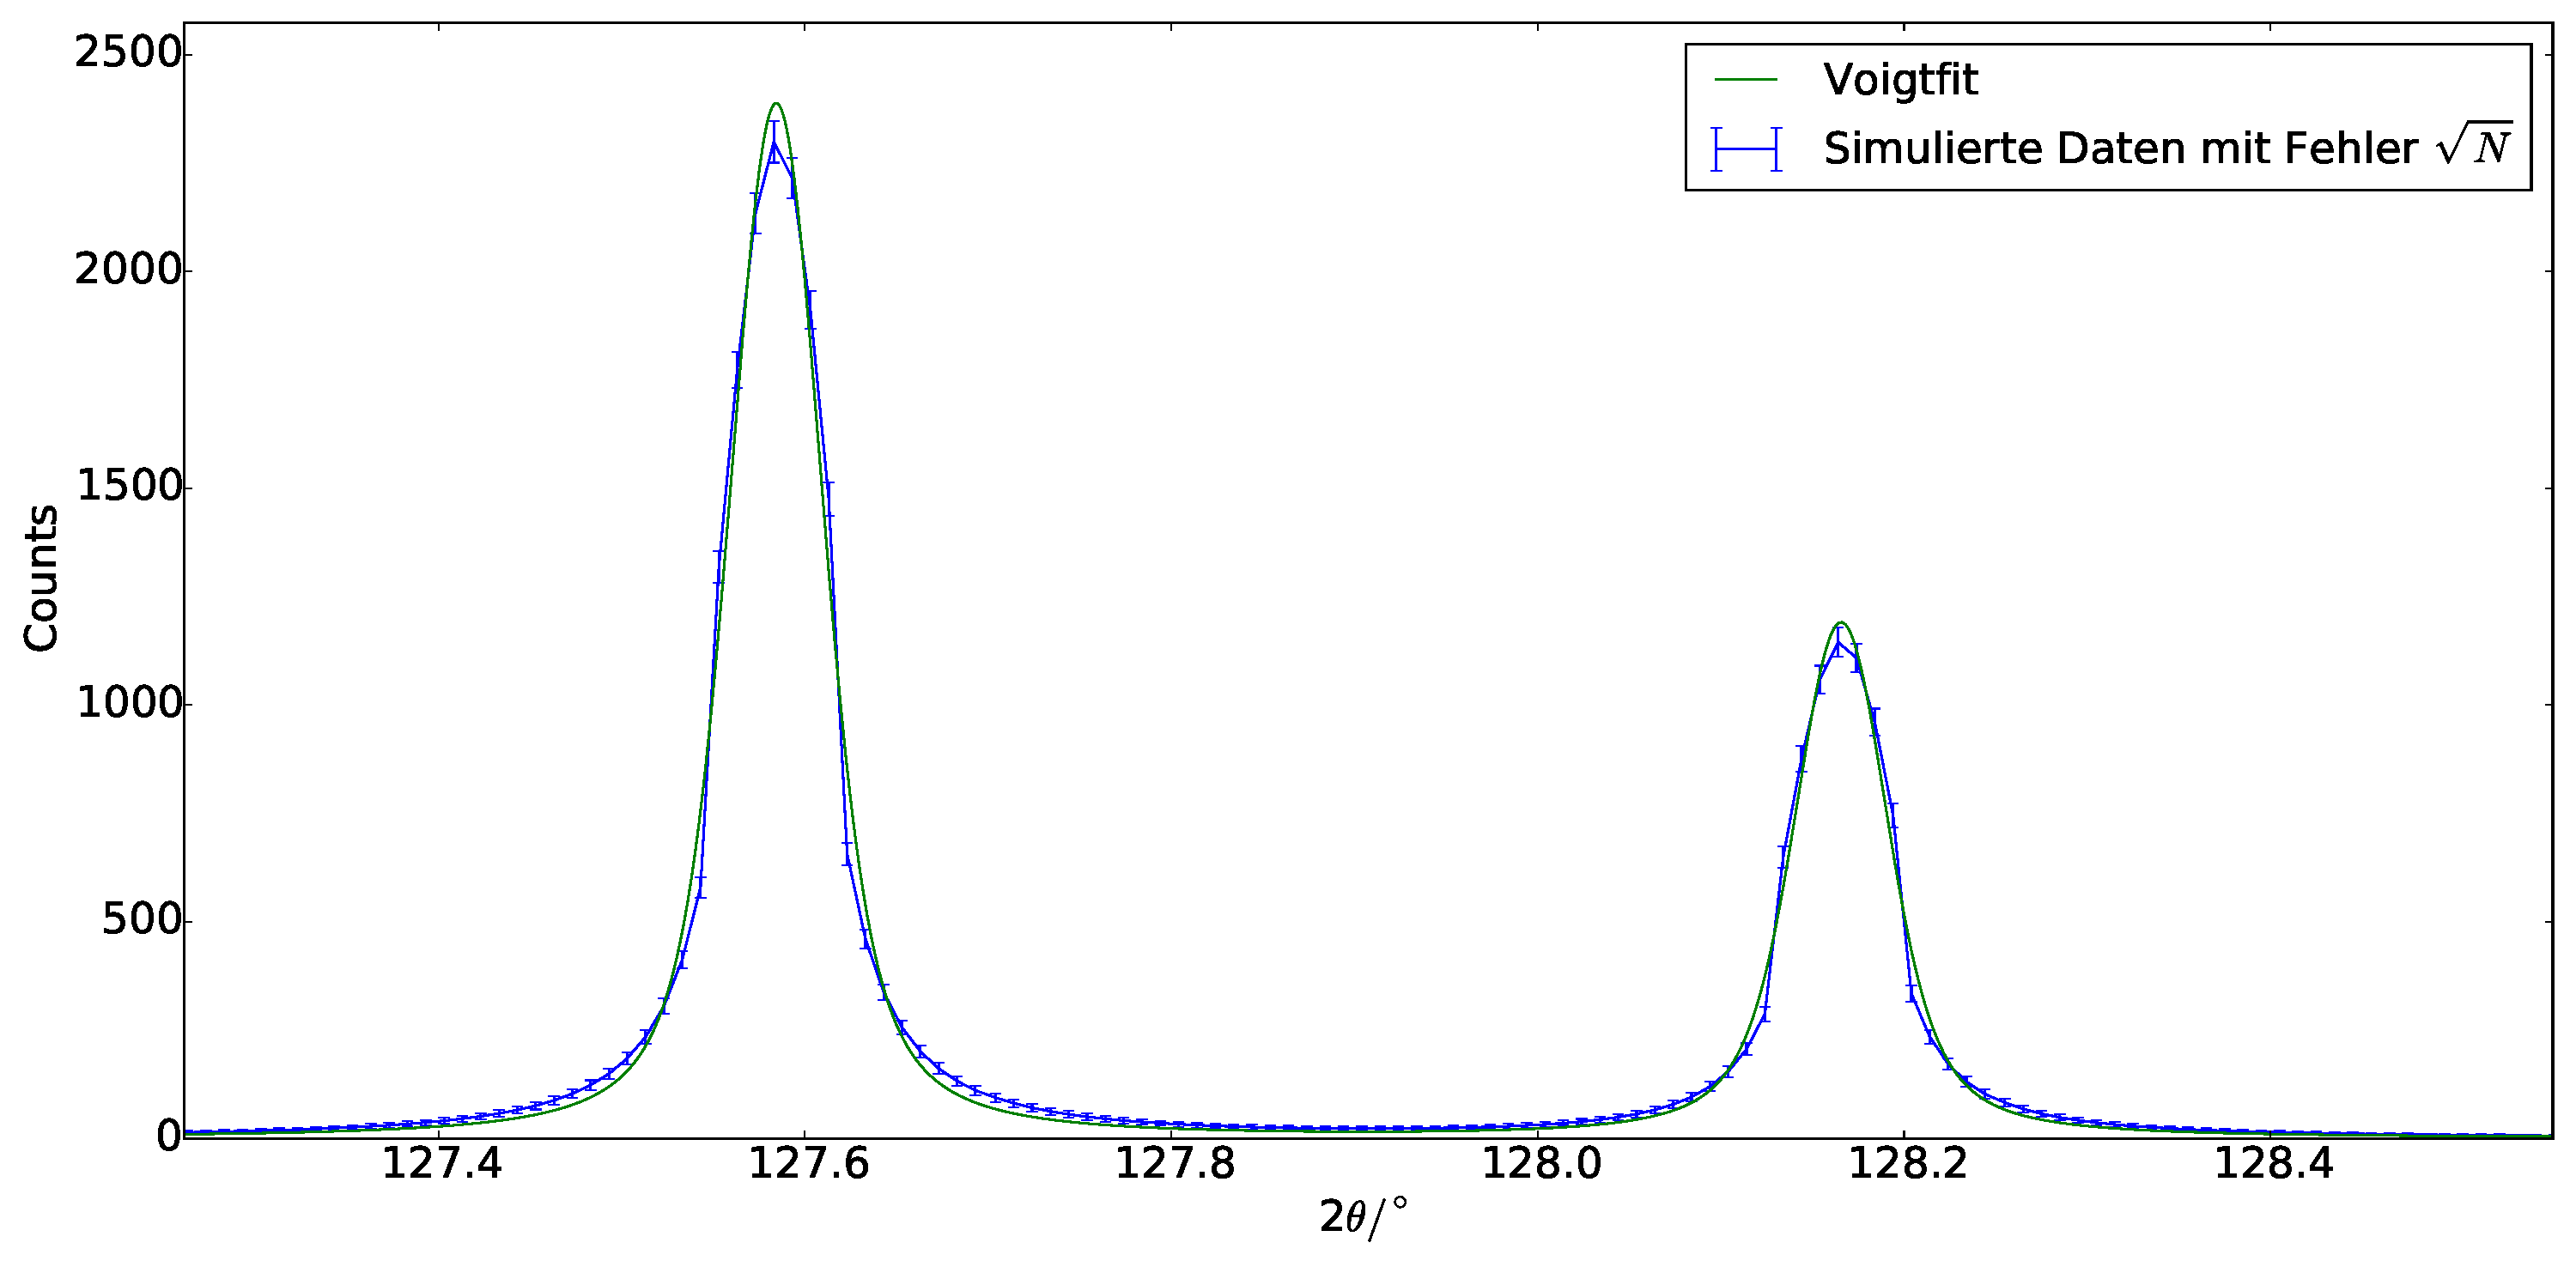
\includegraphics[scale=0.15]{Simulation_Siliciumpulver_10}
  \captionof{figure}{Siliciumpulver 10. Doppelpeak}
  \label{fig:pul_sim_sil_10}
\end{minipage}
\end{figure}
\begin{figure}[H]
\begin{minipage}{.5\textwidth}
  \centering
  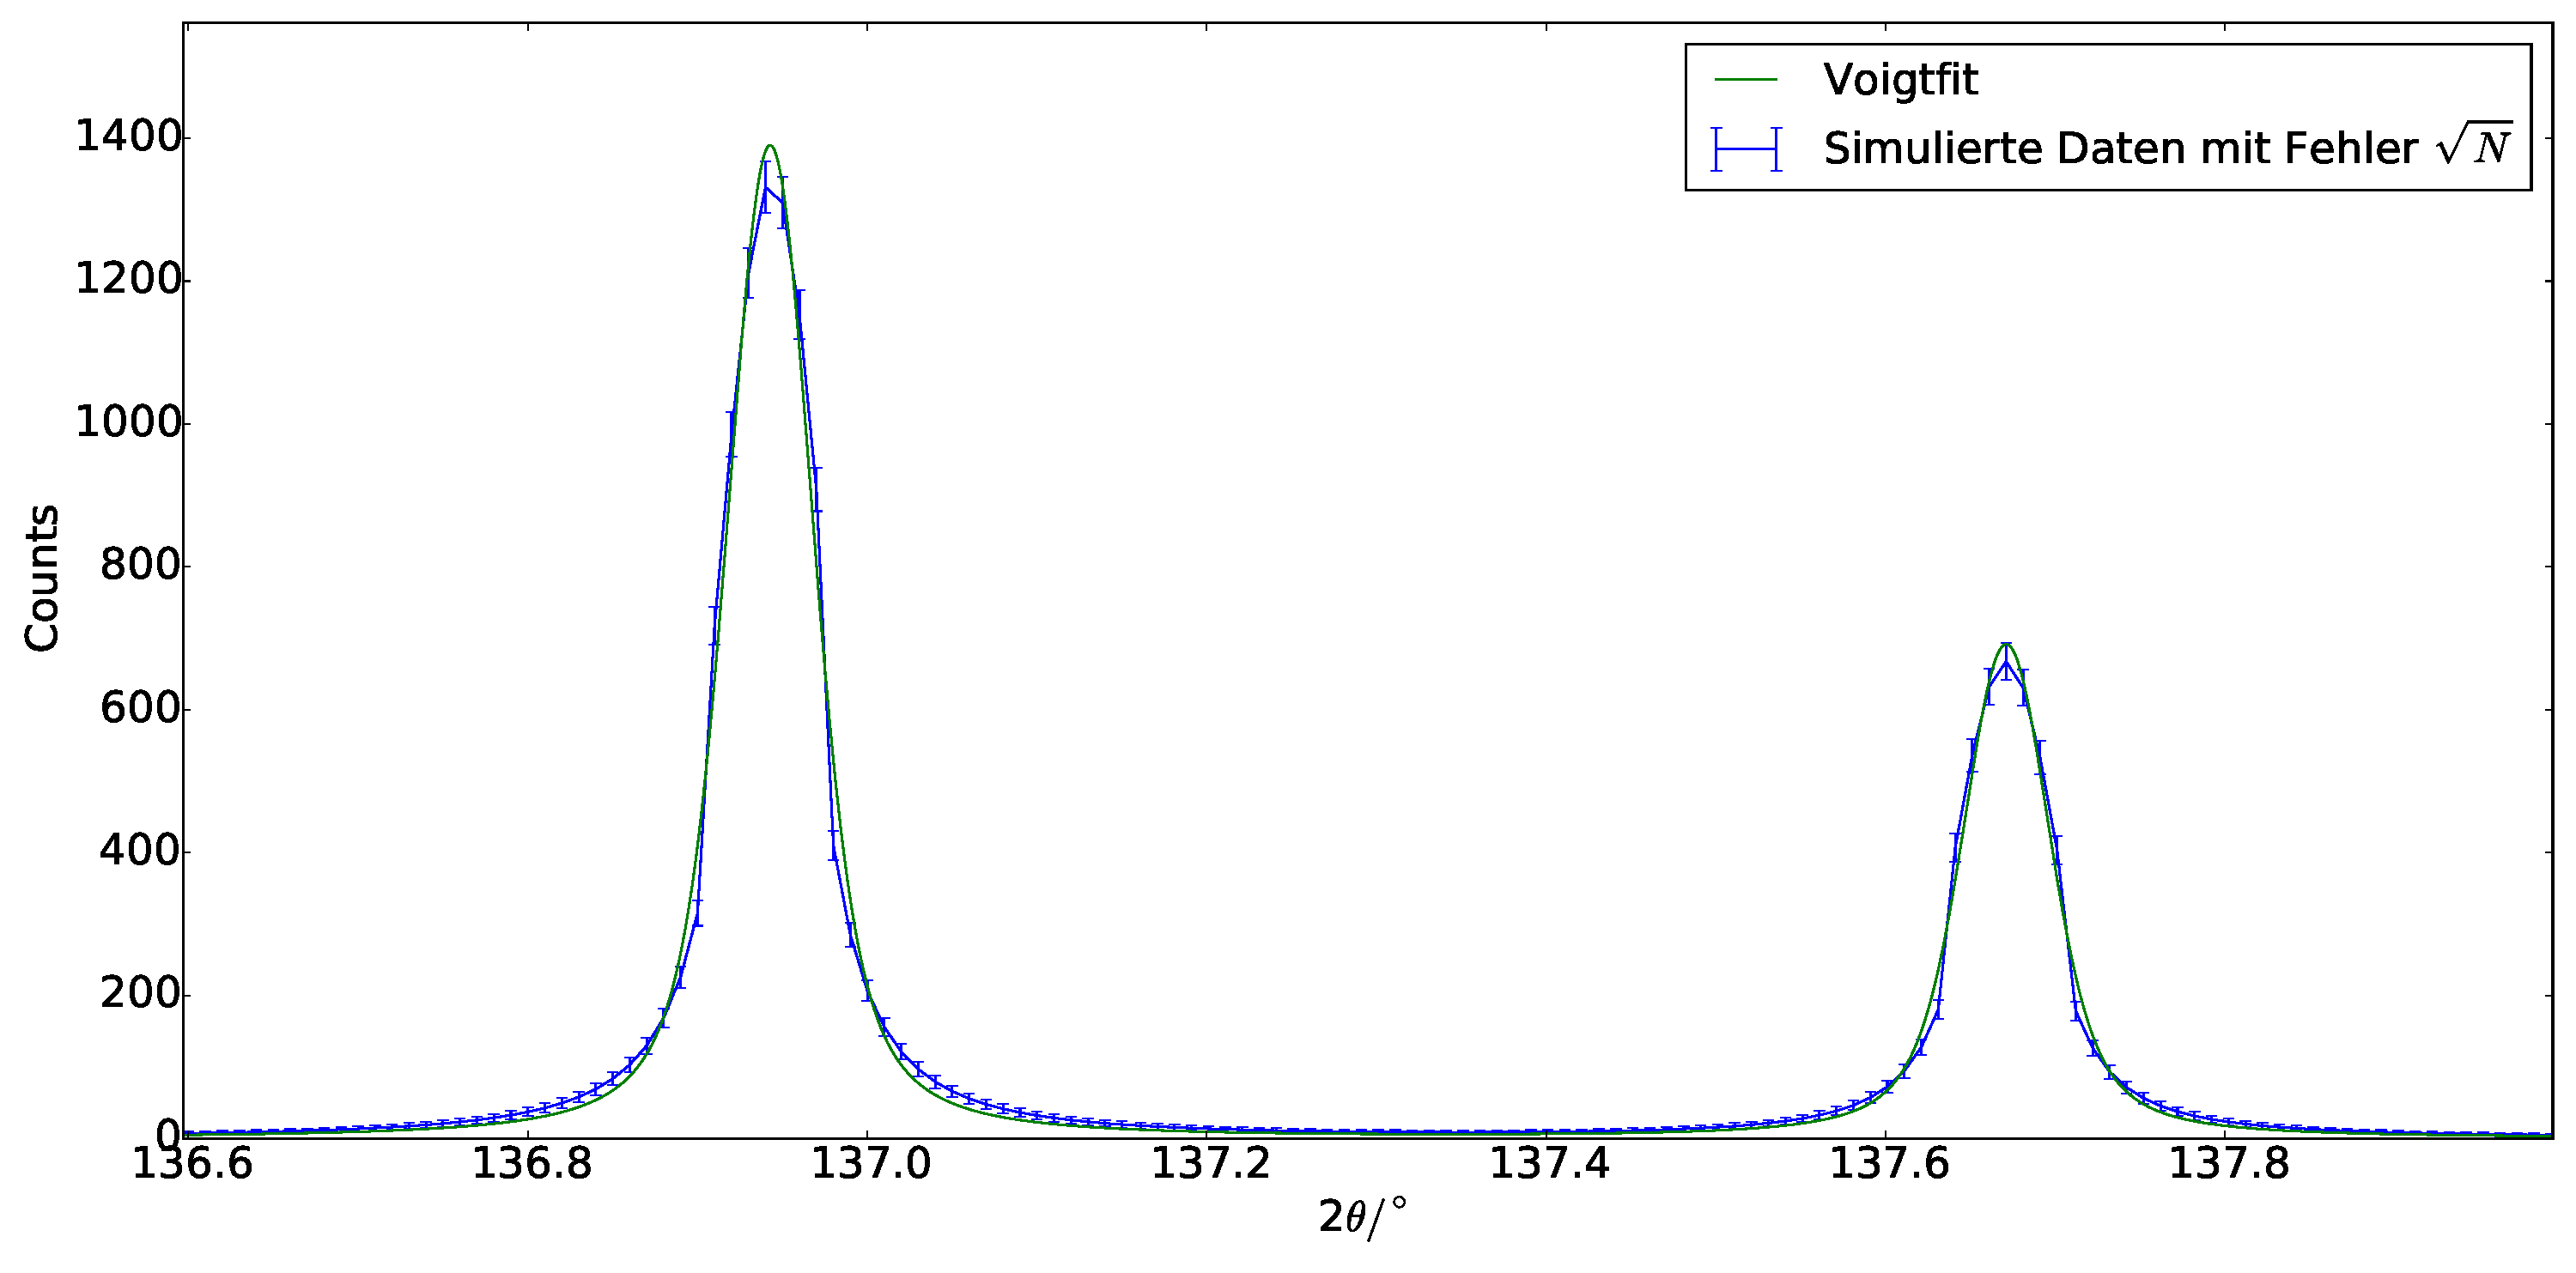
\includegraphics[scale=0.15]{Simulation_Siliciumpulver_11}
  \captionof{figure}{Siliciumpulver 11. Doppelpeak}
  \label{fig:pul_sim_sil_11}
\end{minipage}
\end{figure}
und die simulierten Peaks von Germanium zu sehen.
\begin{figure}[H]
\begin{minipage}{.5\textwidth}
  \centering
  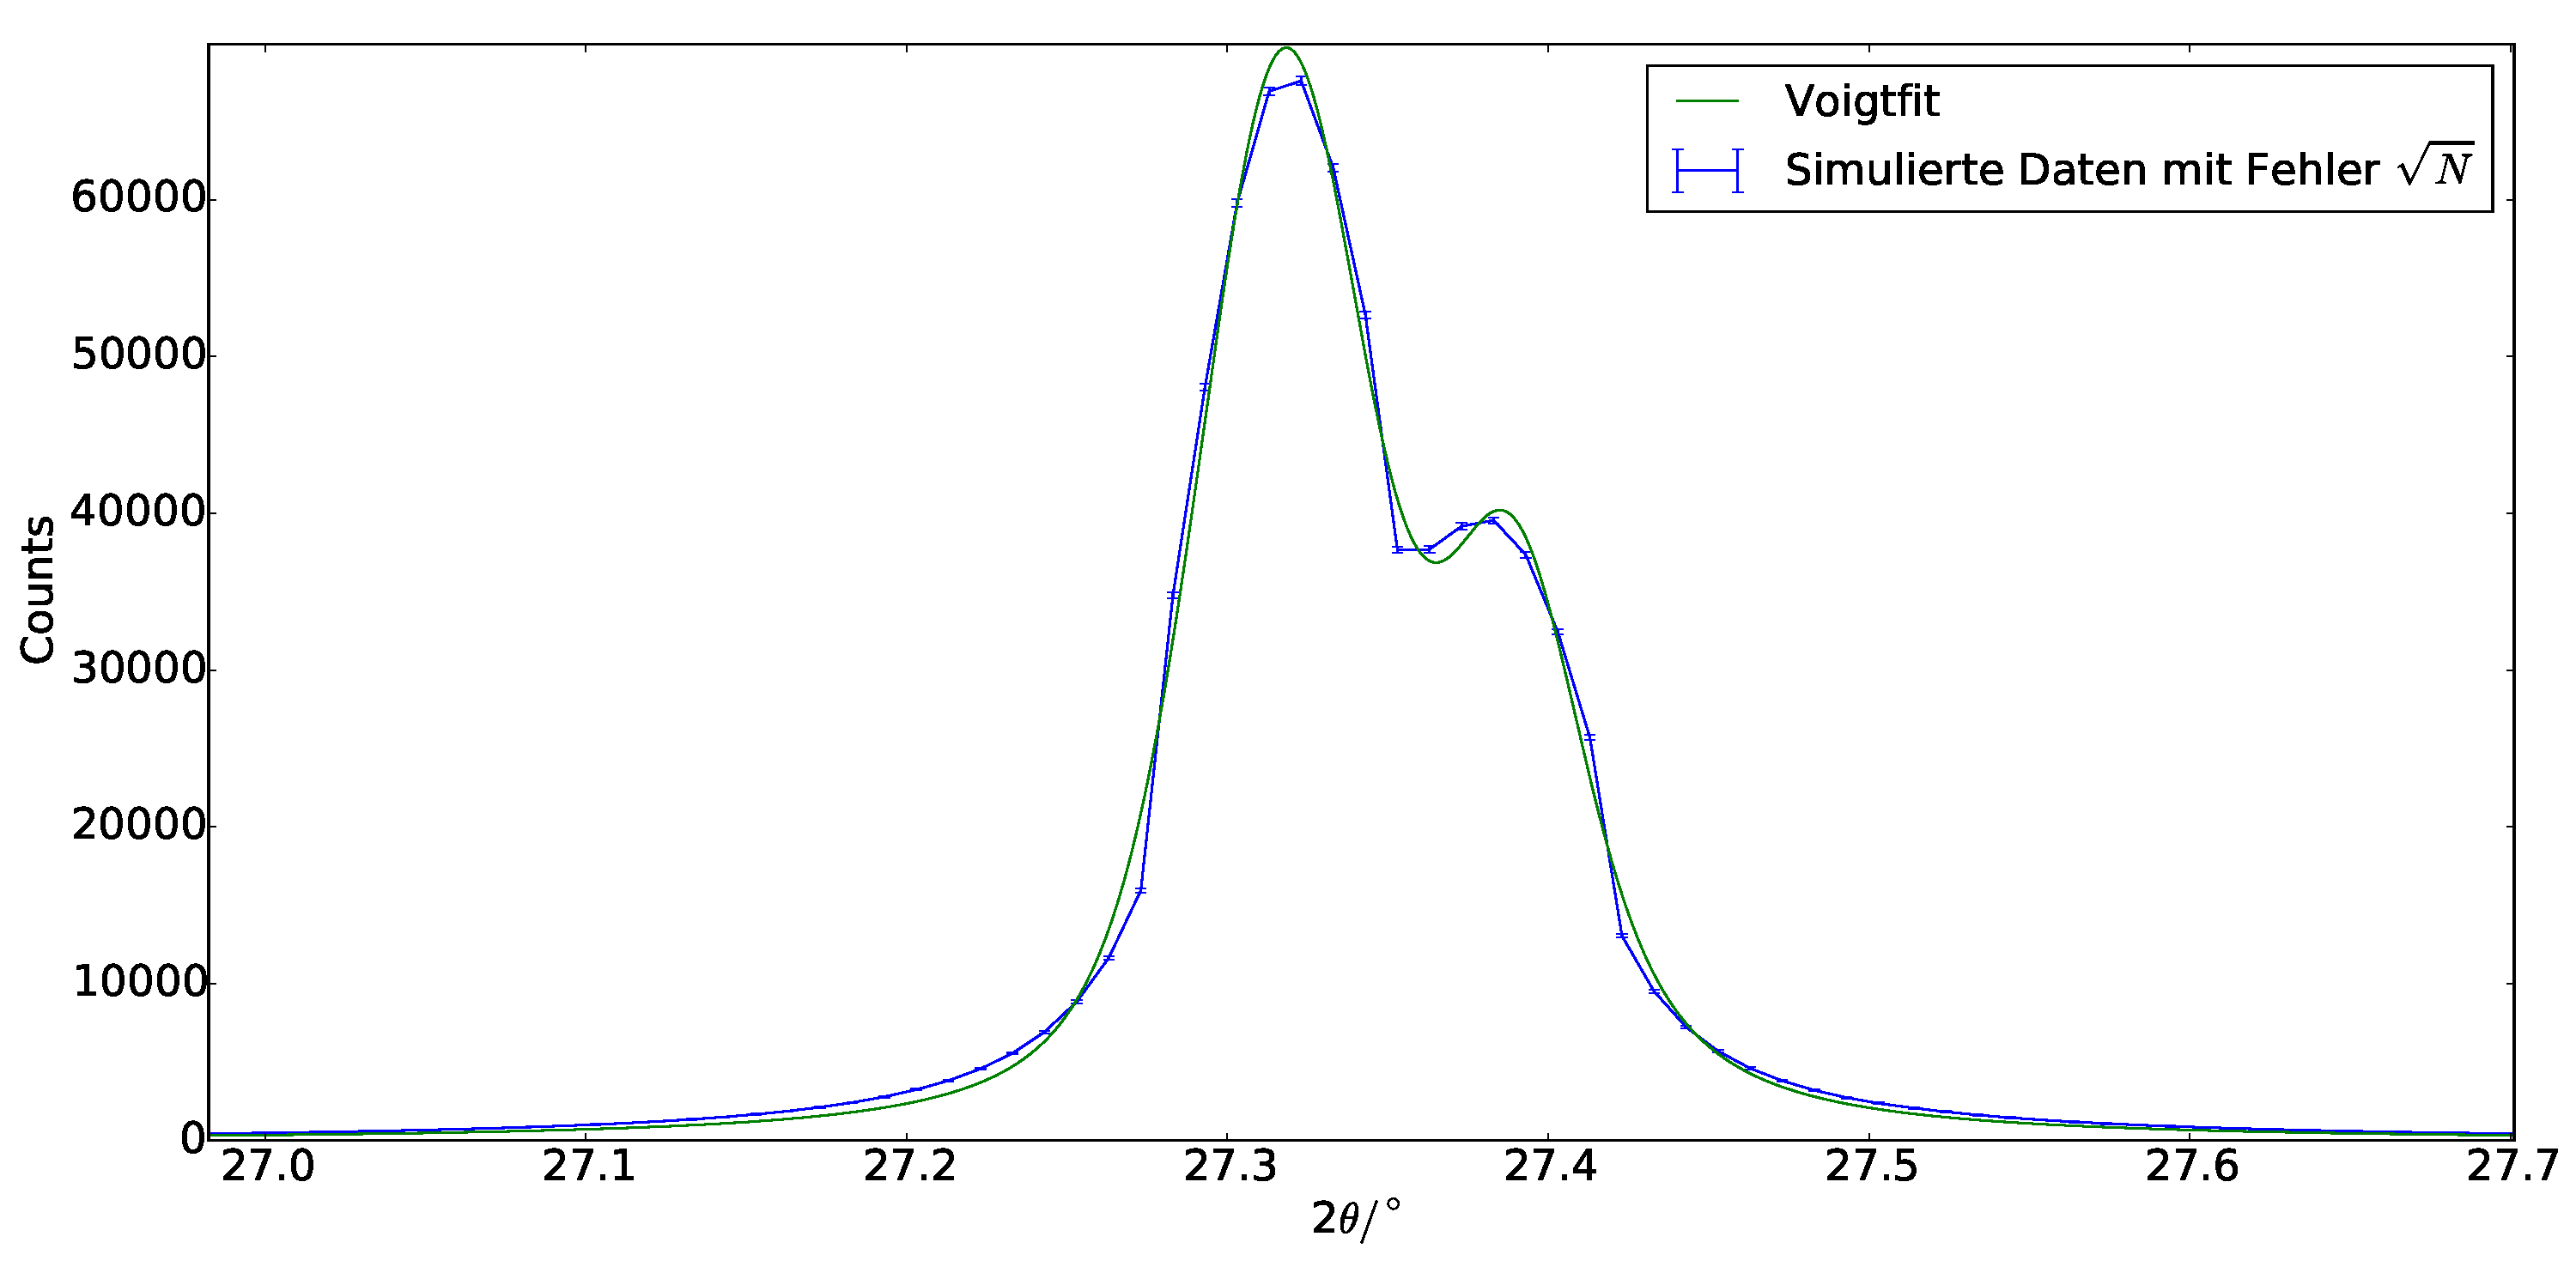
\includegraphics[scale=0.15]{Simulation_Germaniumpulver_1}
  \captionof{figure}{Germaniumpulver 1. Doppelpeak}
  \label{fig:pul_sim_ger_1}
\end{minipage}
\hspace{0.5cm}
\begin{minipage}{.5\textwidth}
  \centering
  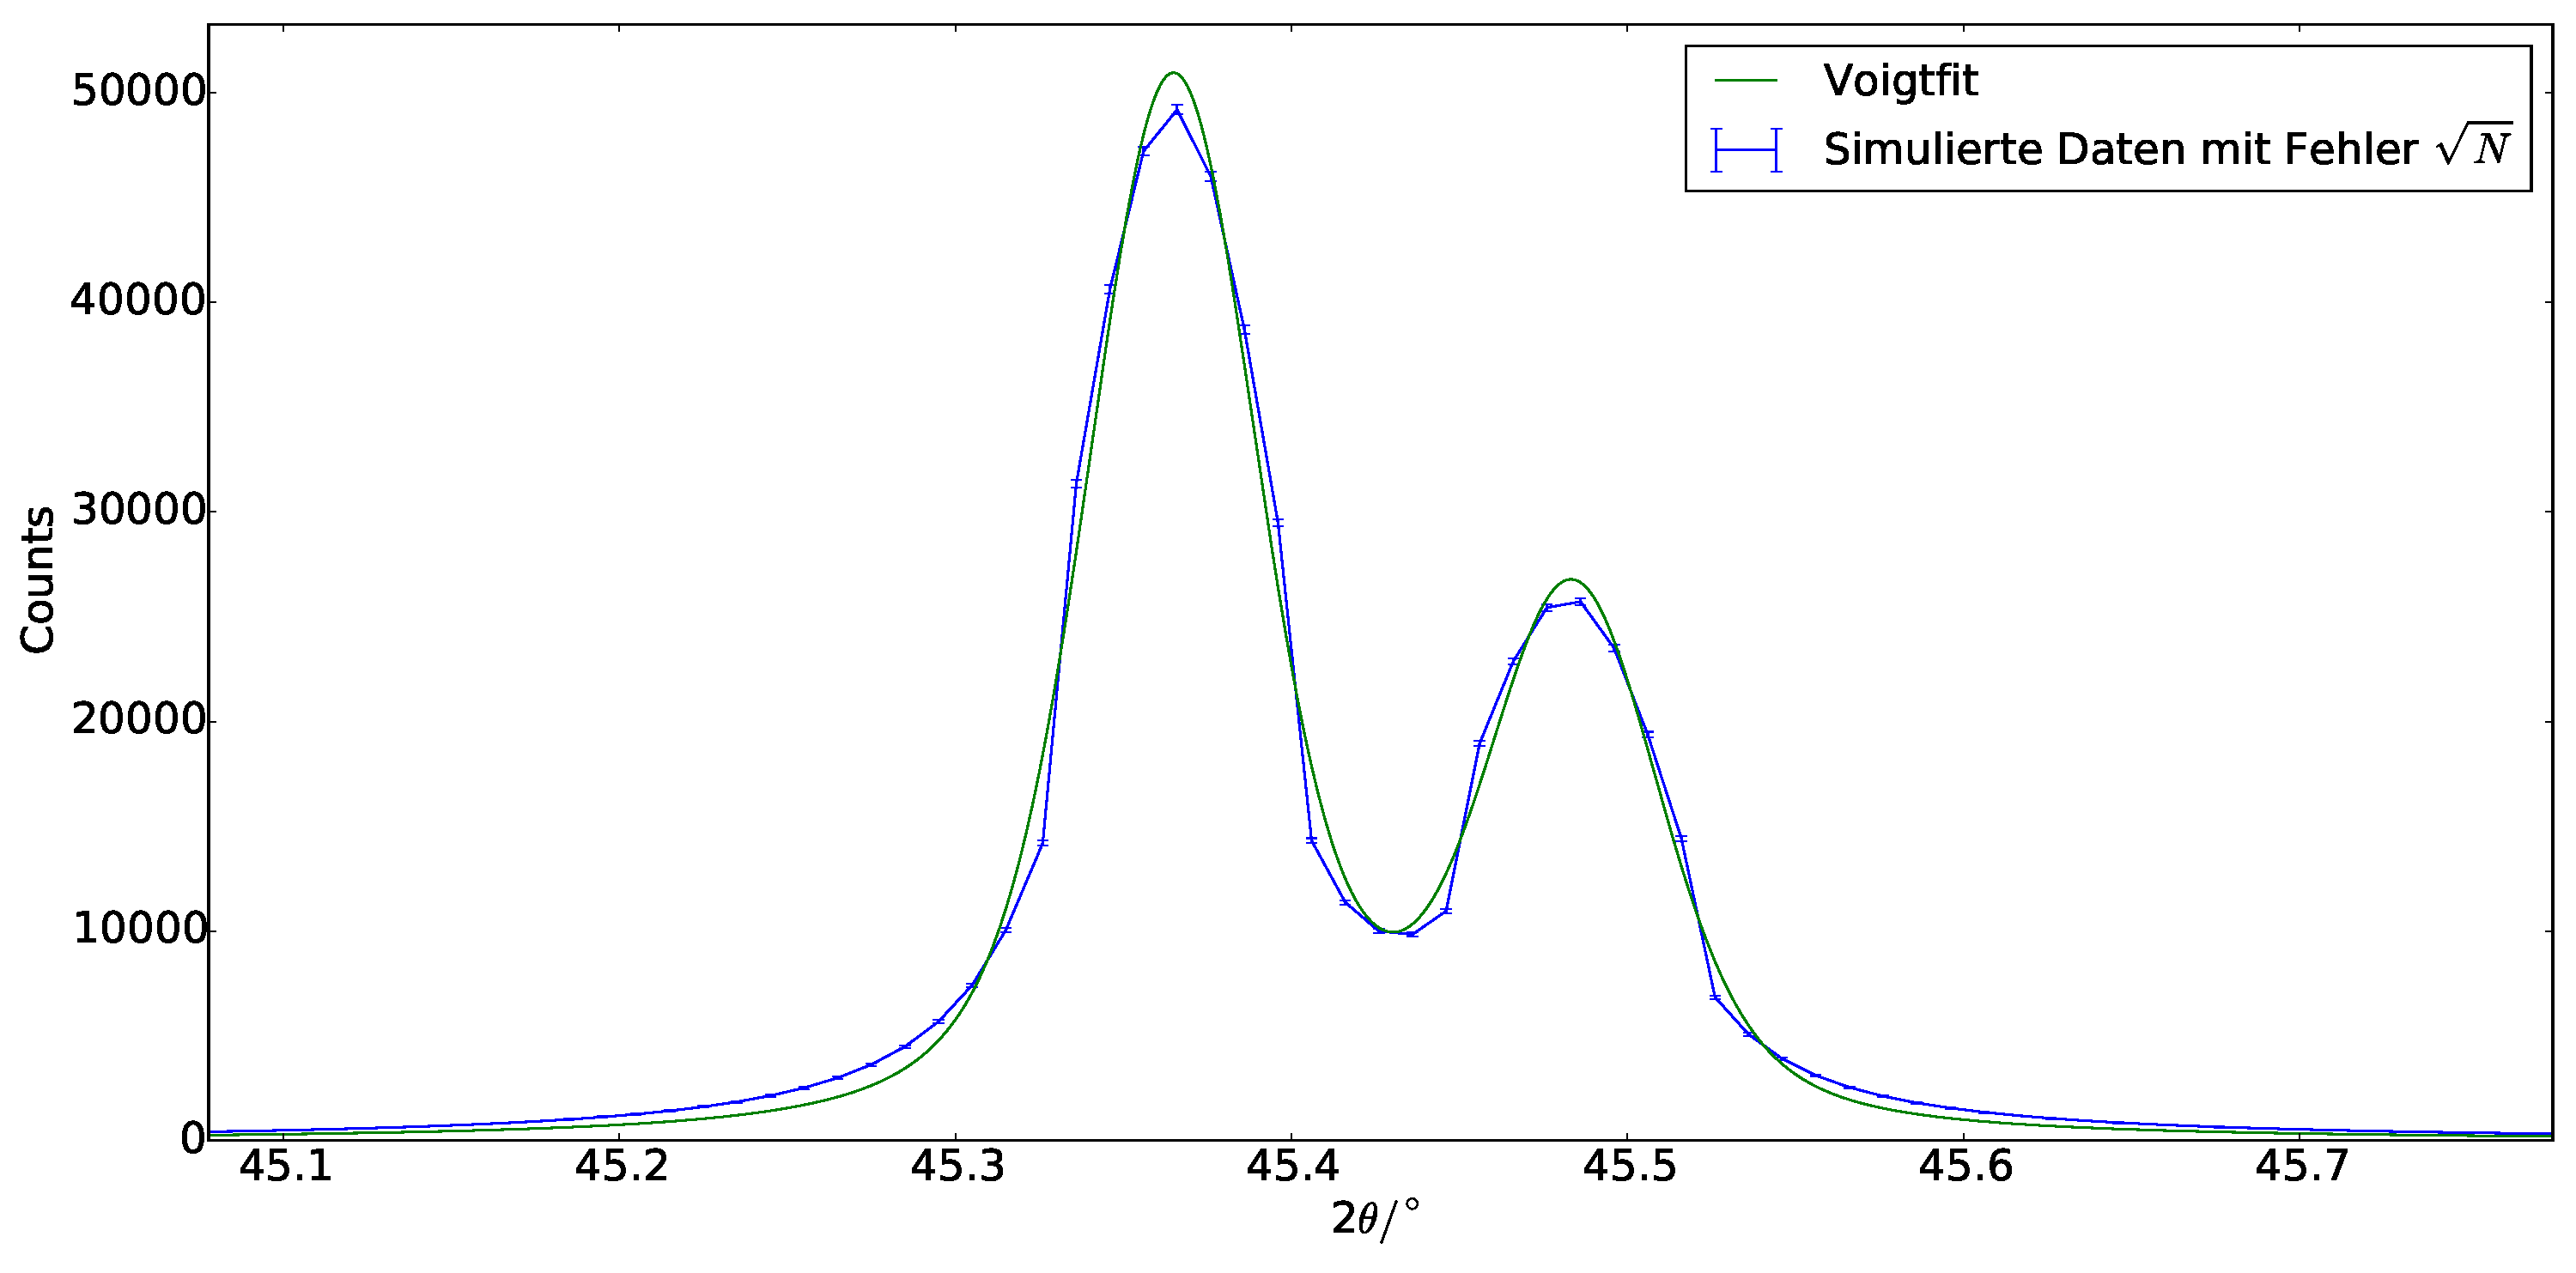
\includegraphics[scale=0.15]{Simulation_Germaniumpulver_2}
  \captionof{figure}{Germaniumpulver 2. Doppelpeak}
  \label{fig:pul_sim_ger_2}
\end{minipage}
\end{figure}
\begin{figure}[H]
\begin{minipage}{.5\textwidth}
  \centering
  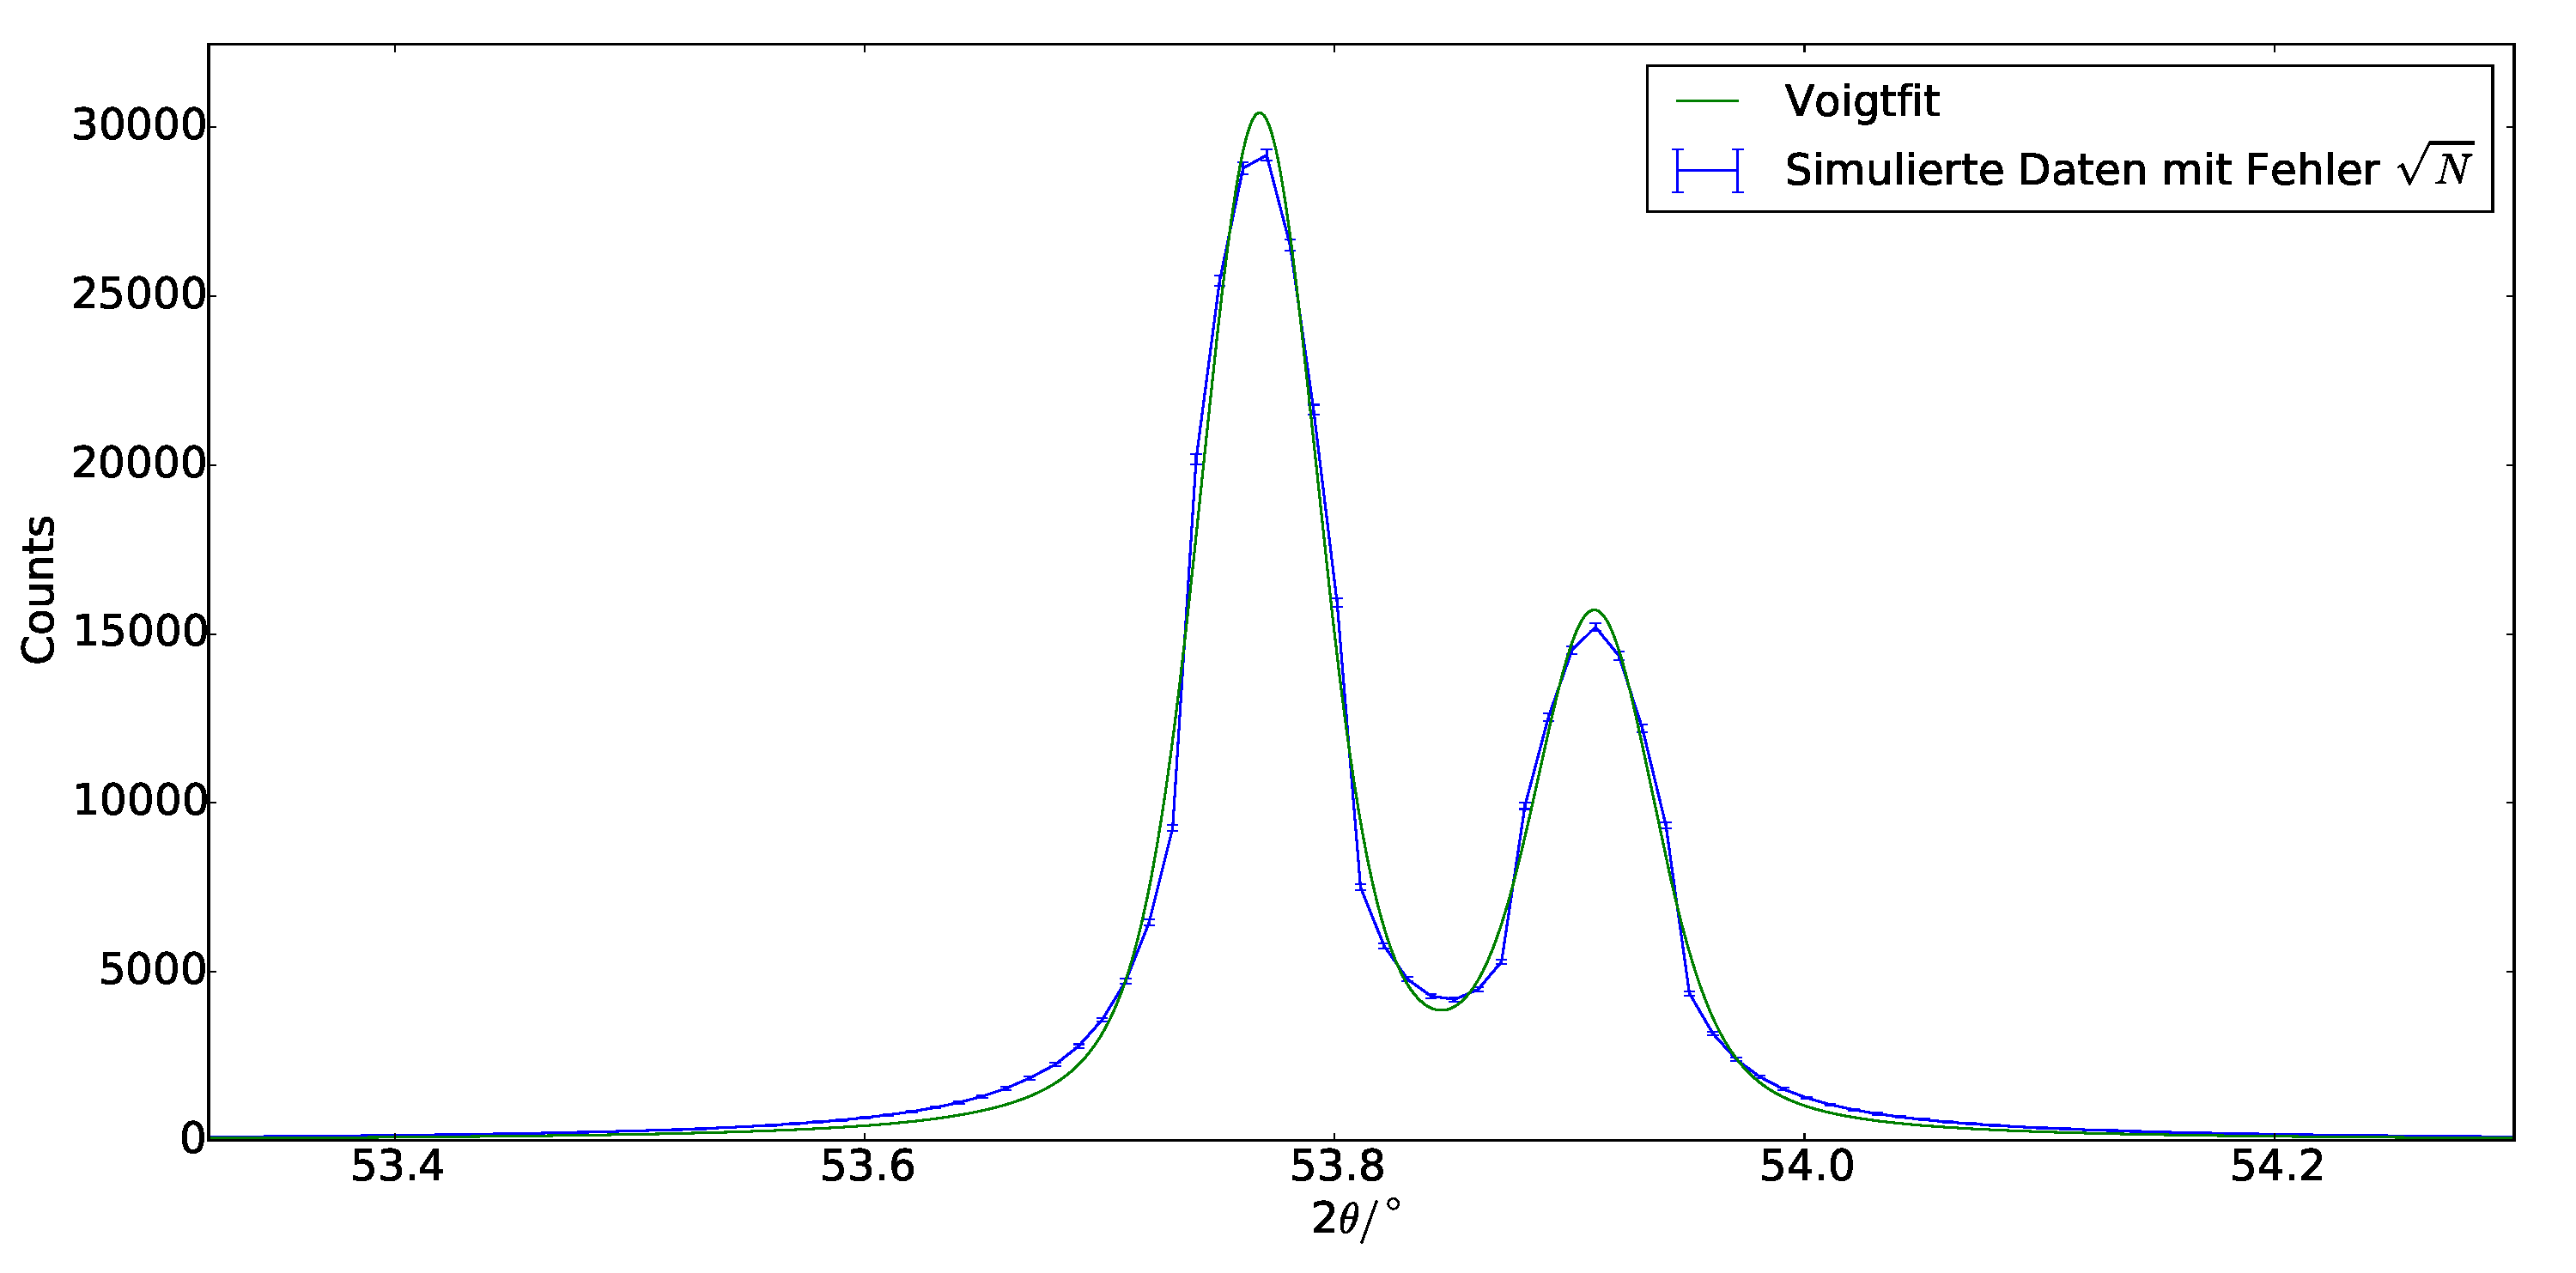
\includegraphics[scale=0.15]{Simulation_Germaniumpulver_3}
  \captionof{figure}{Germaniumpulver 3. Doppelpeak}
  \label{fig:pul_sim_ger_3}
\end{minipage}
\hspace{0.5cm}
\begin{minipage}{.5\textwidth}
  \centering
  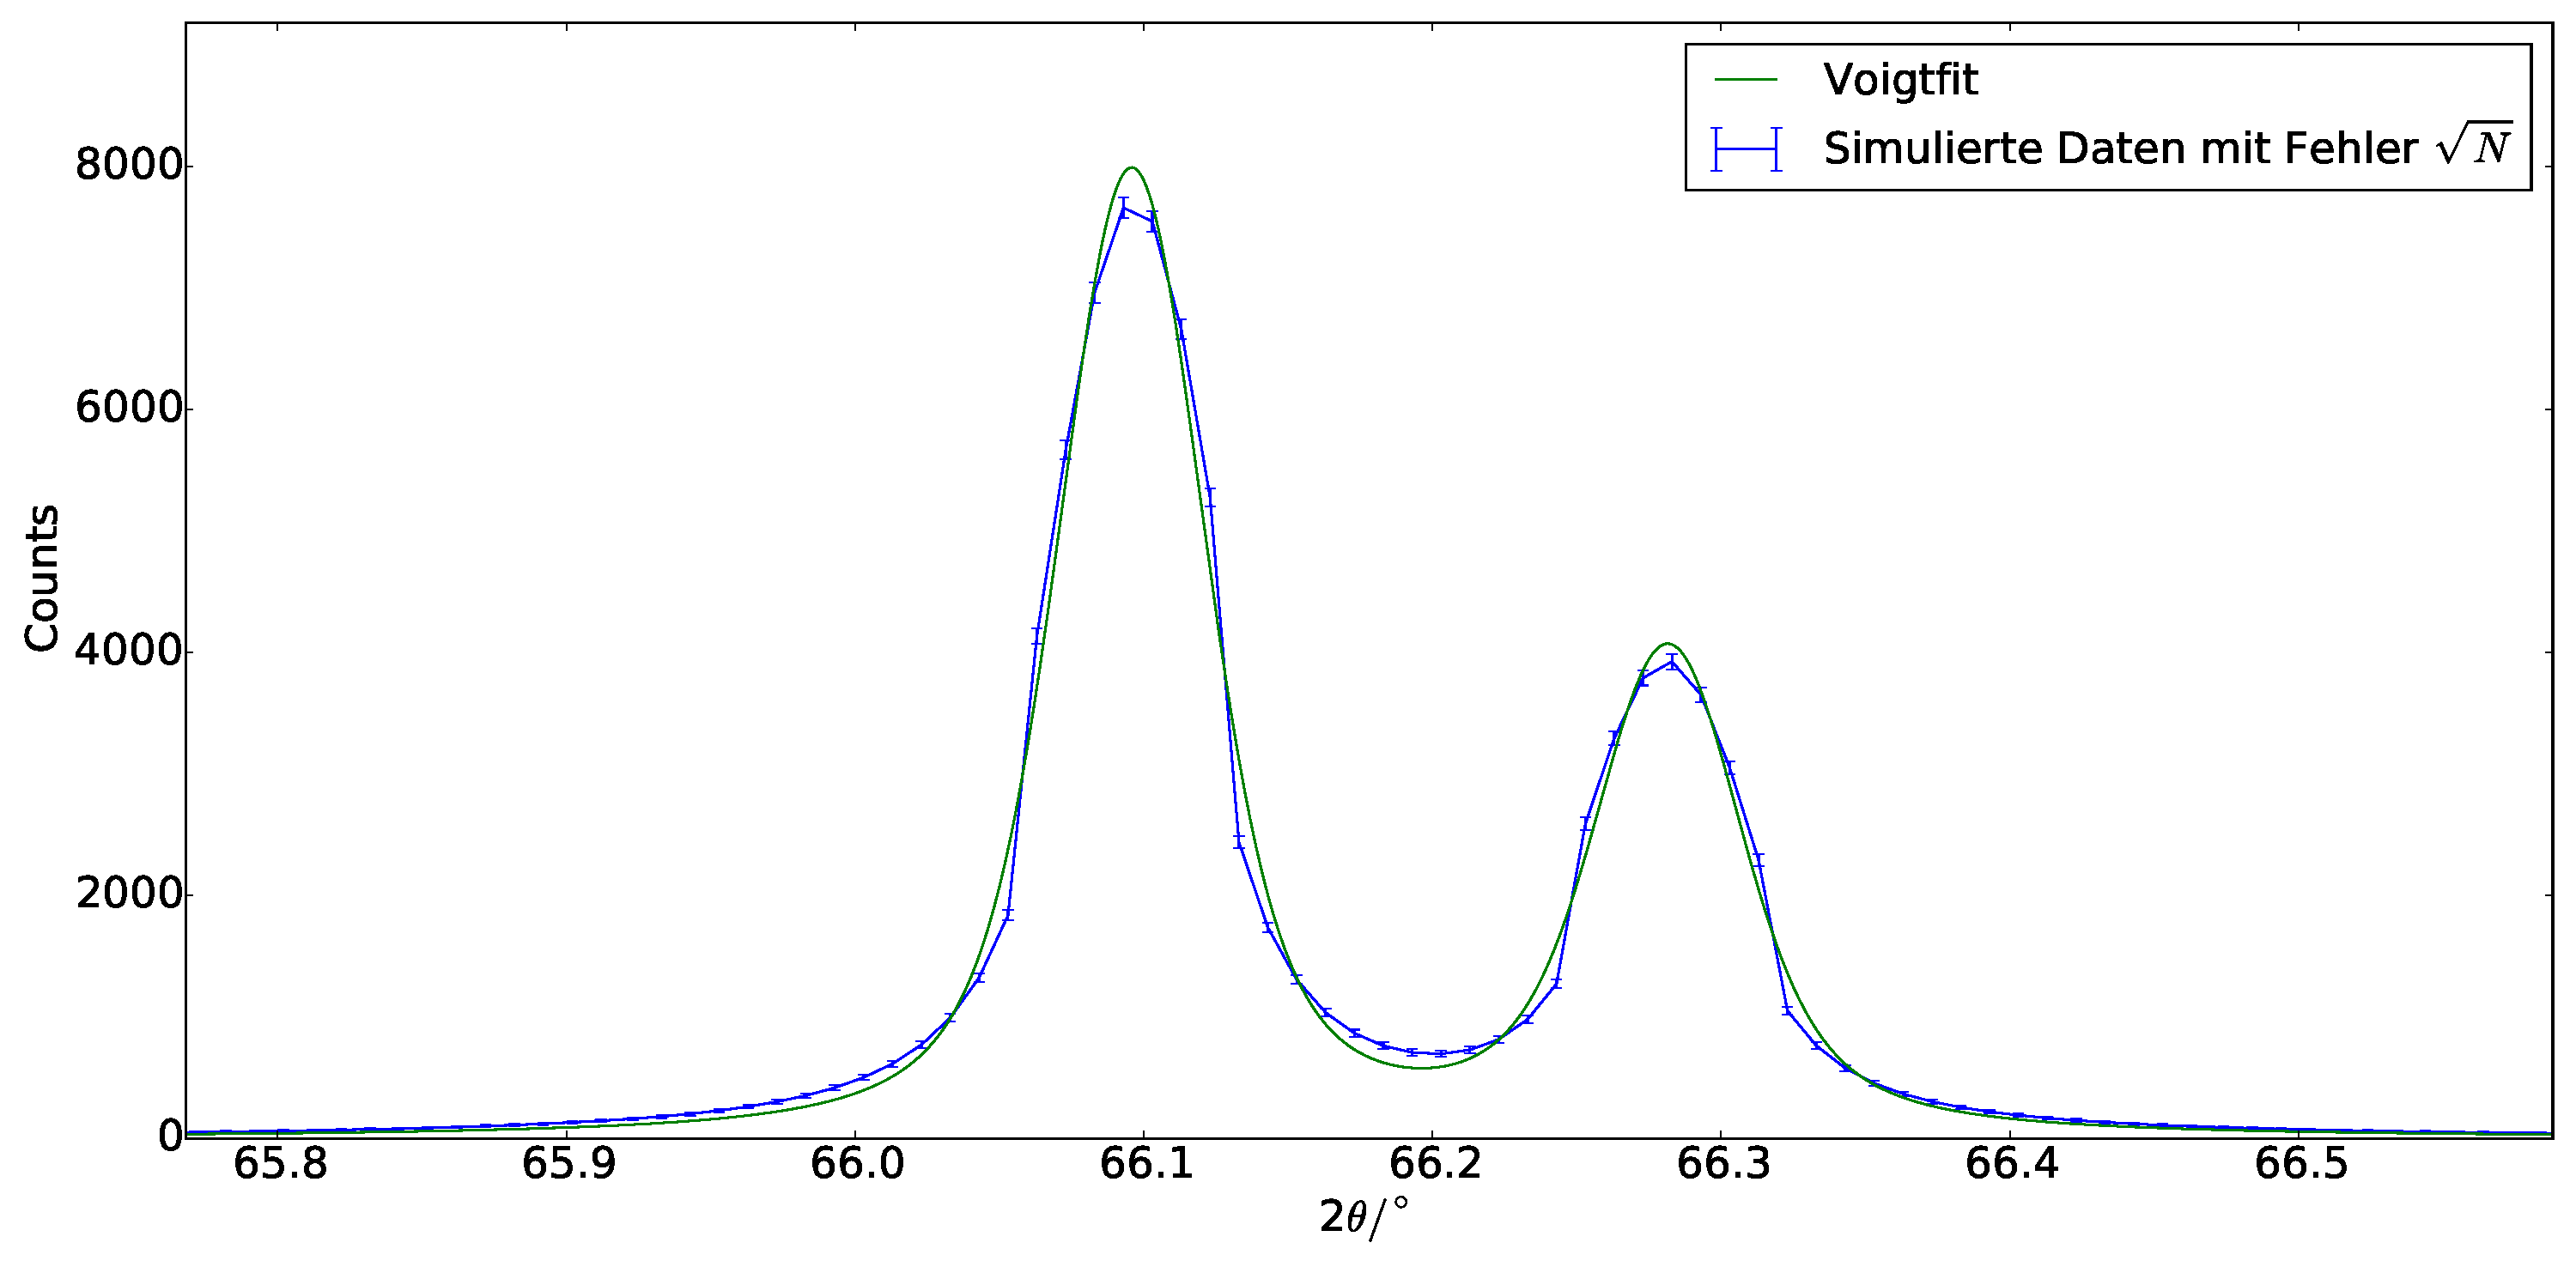
\includegraphics[scale=0.15]{Simulation_Germaniumpulver_4}
  \captionof{figure}{Germaniumpulver 4. Doppelpeak}
  \label{fig:pul_sim_ger_4}
\end{minipage}
\end{figure}
\begin{figure}[H]
\begin{minipage}{.5\textwidth}
  \centering
  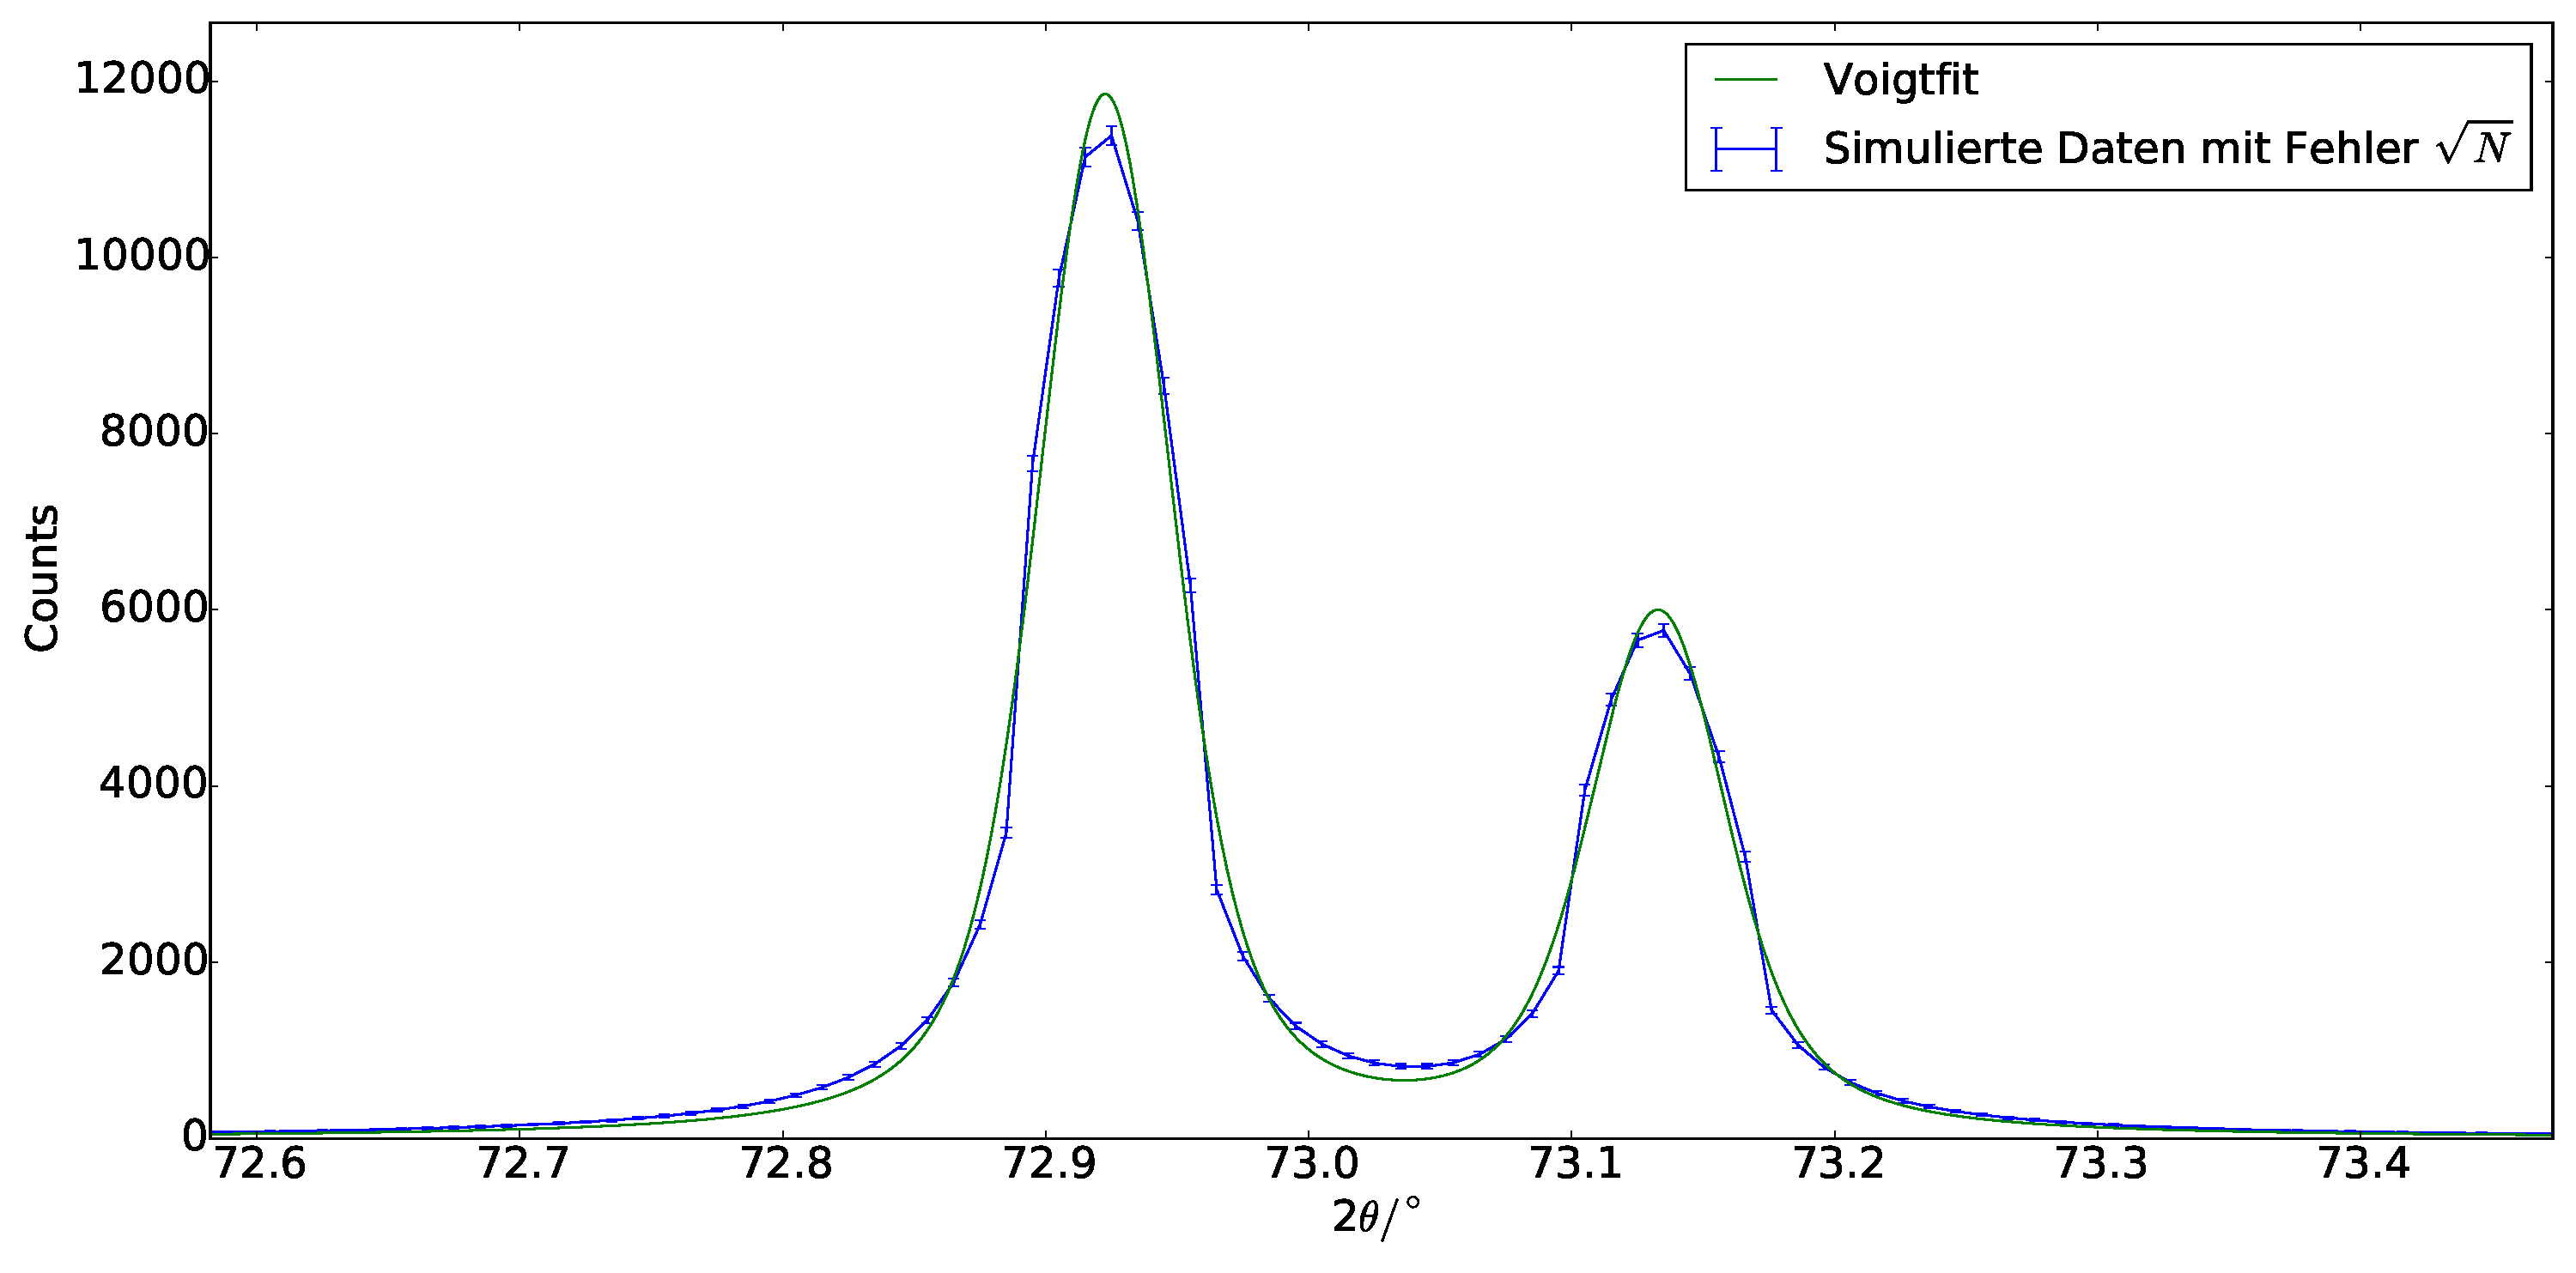
\includegraphics[scale=0.15]{Simulation_Germaniumpulver_5}
  \captionof{figure}{Germaniumpulver 5. Doppelpeak}
  \label{fig:pul_sim_ger_5}
\end{minipage}
\hspace{0.5cm}
\begin{minipage}{.5\textwidth}
  \centering
  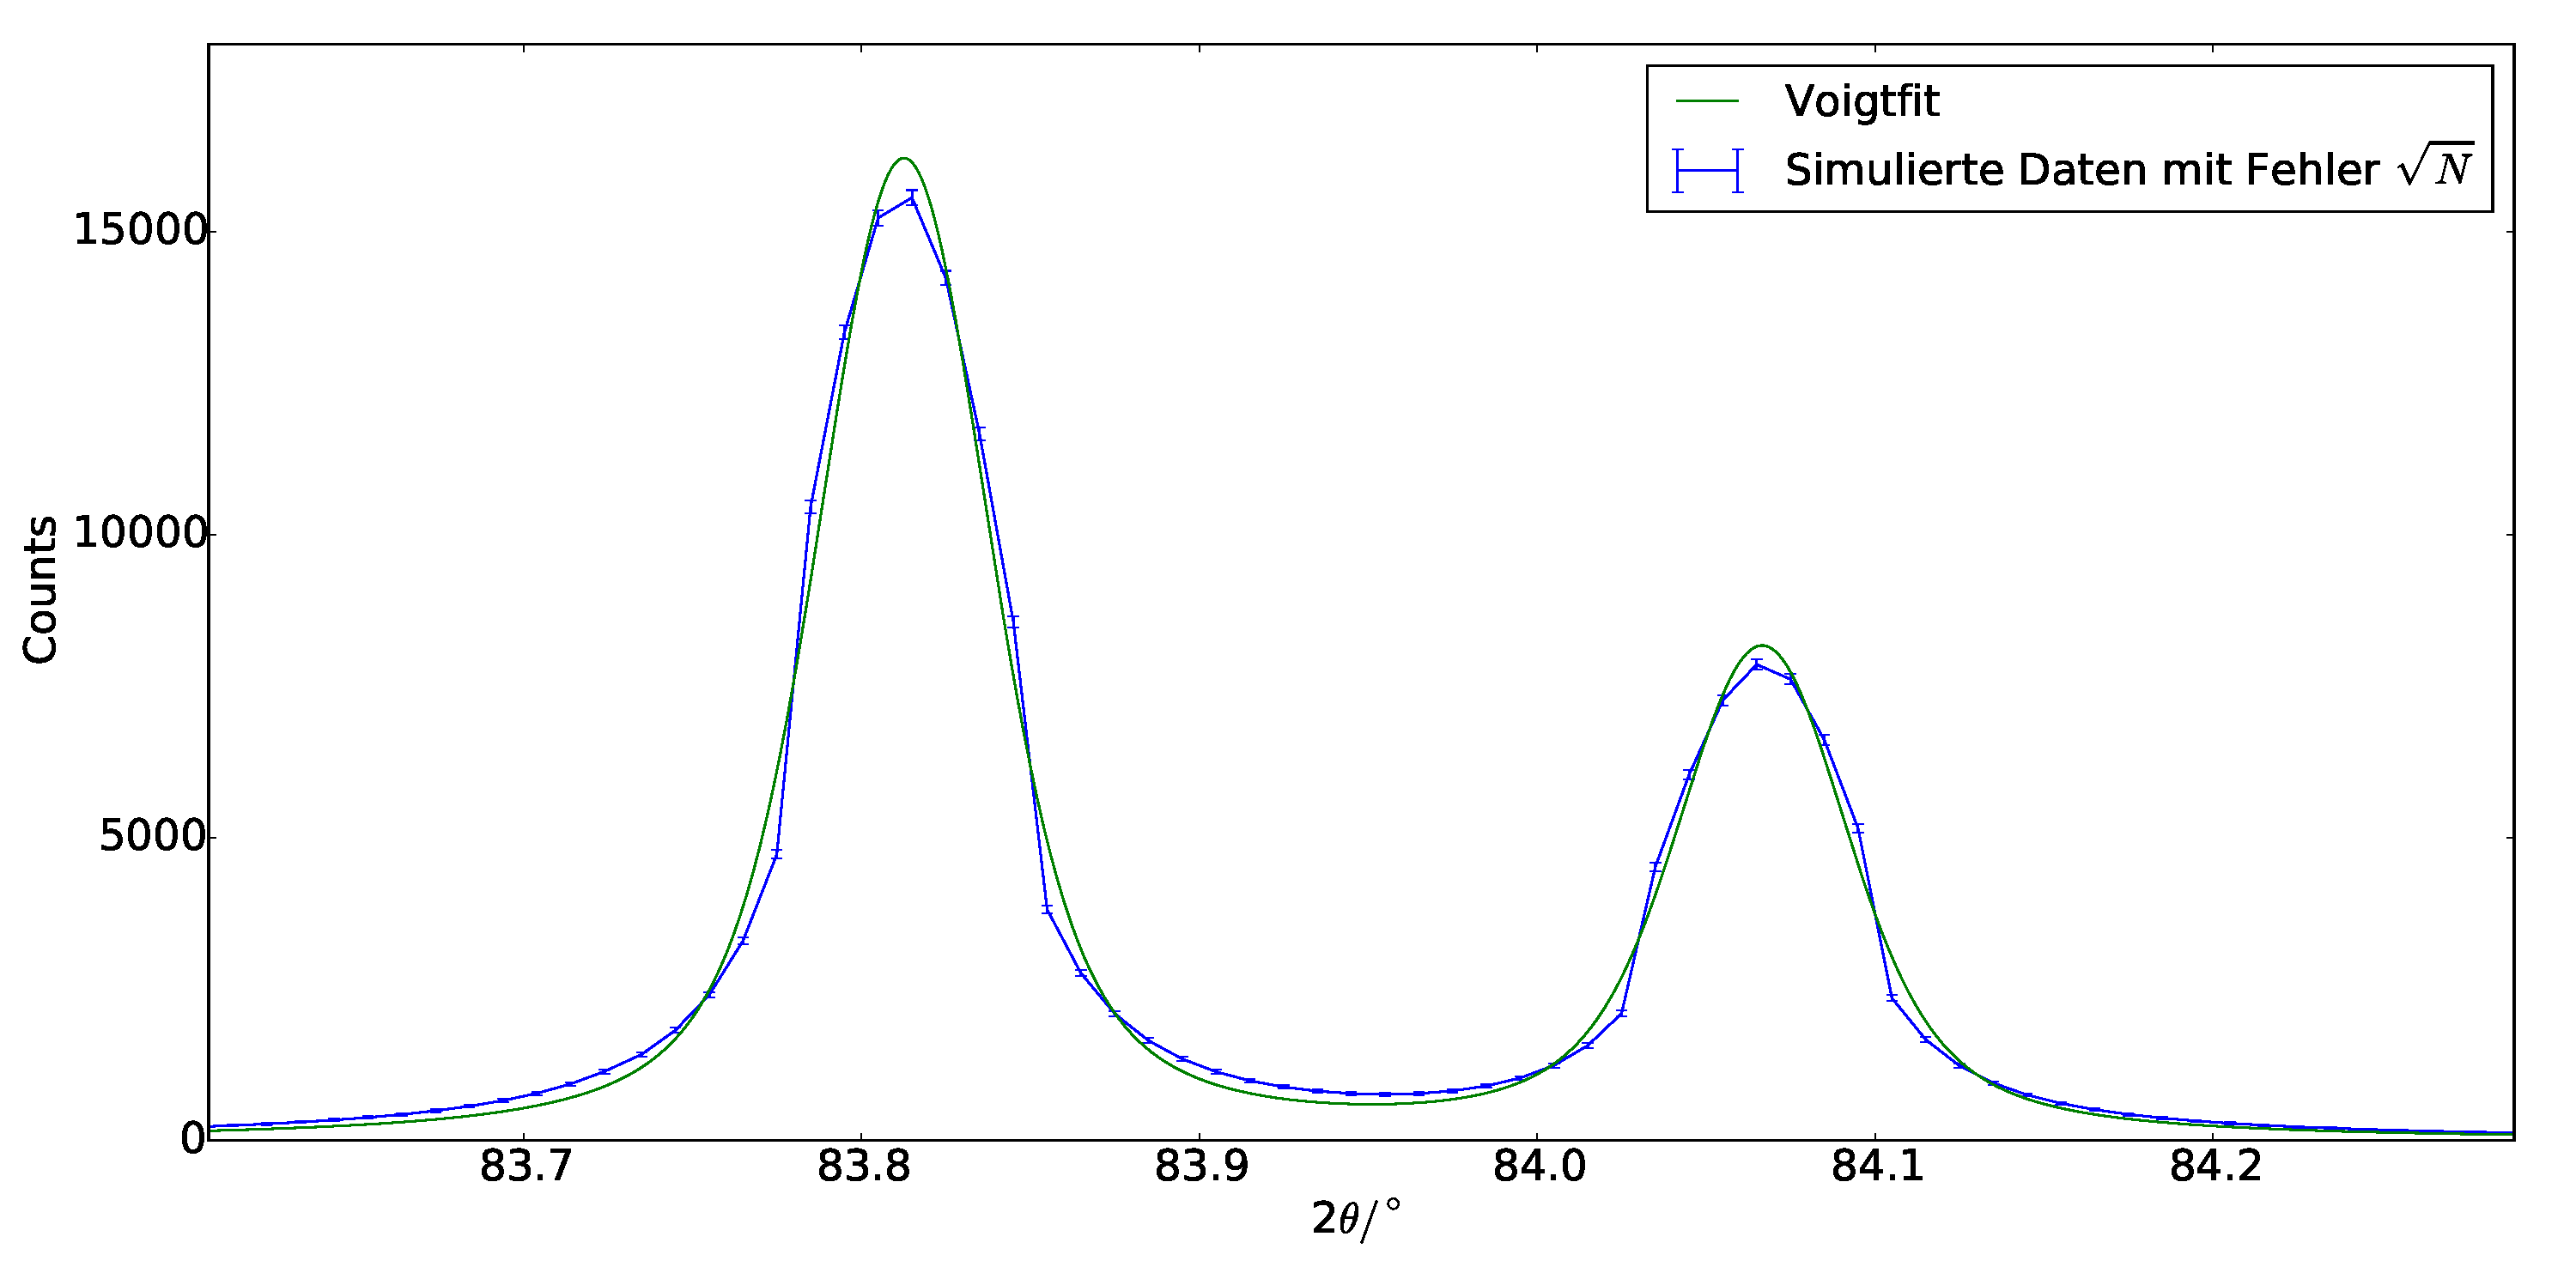
\includegraphics[scale=0.15]{Simulation_Germaniumpulver_6}
  \captionof{figure}{Germaniumpulver 6. Doppelpeak}
  \label{fig:pul_sim_ger_6}
\end{minipage}
\end{figure}
\begin{figure}[H]
\begin{minipage}{.5\textwidth}
  \centering
  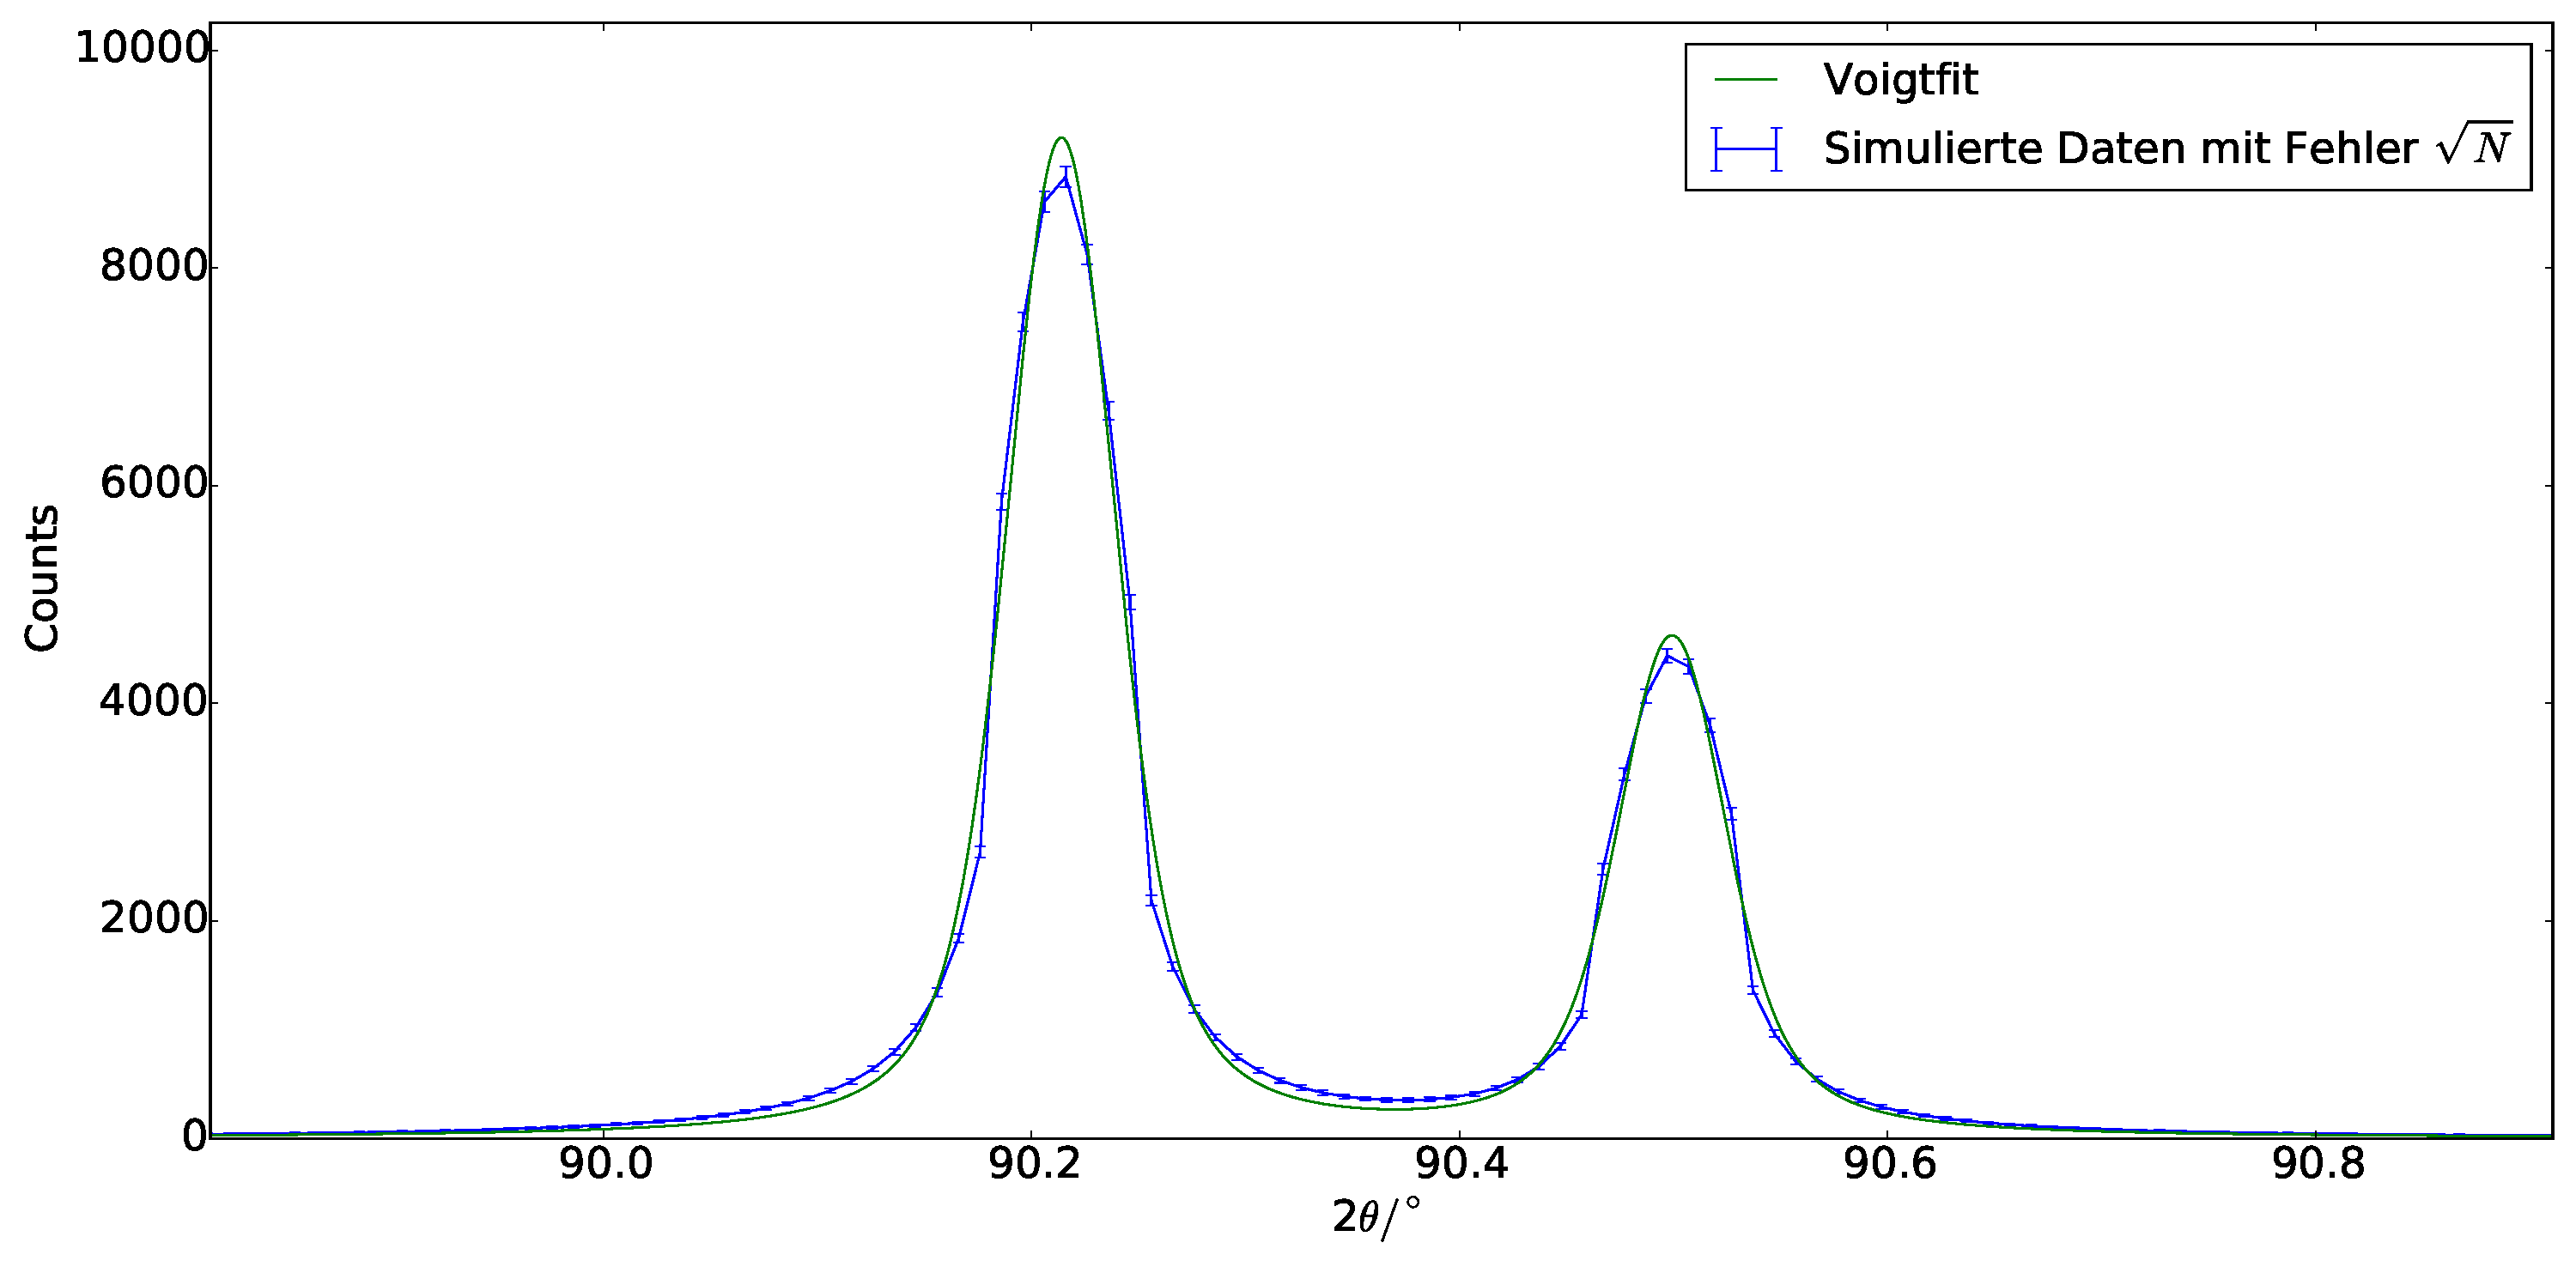
\includegraphics[scale=0.15]{Simulation_Germaniumpulver_7}
  \captionof{figure}{Germaniumpulver 7. Doppelpeak}
  \label{fig:pul_sim_ger_7}
\end{minipage}
\hspace{0.5cm}
\begin{minipage}{.5\textwidth}
  \centering
  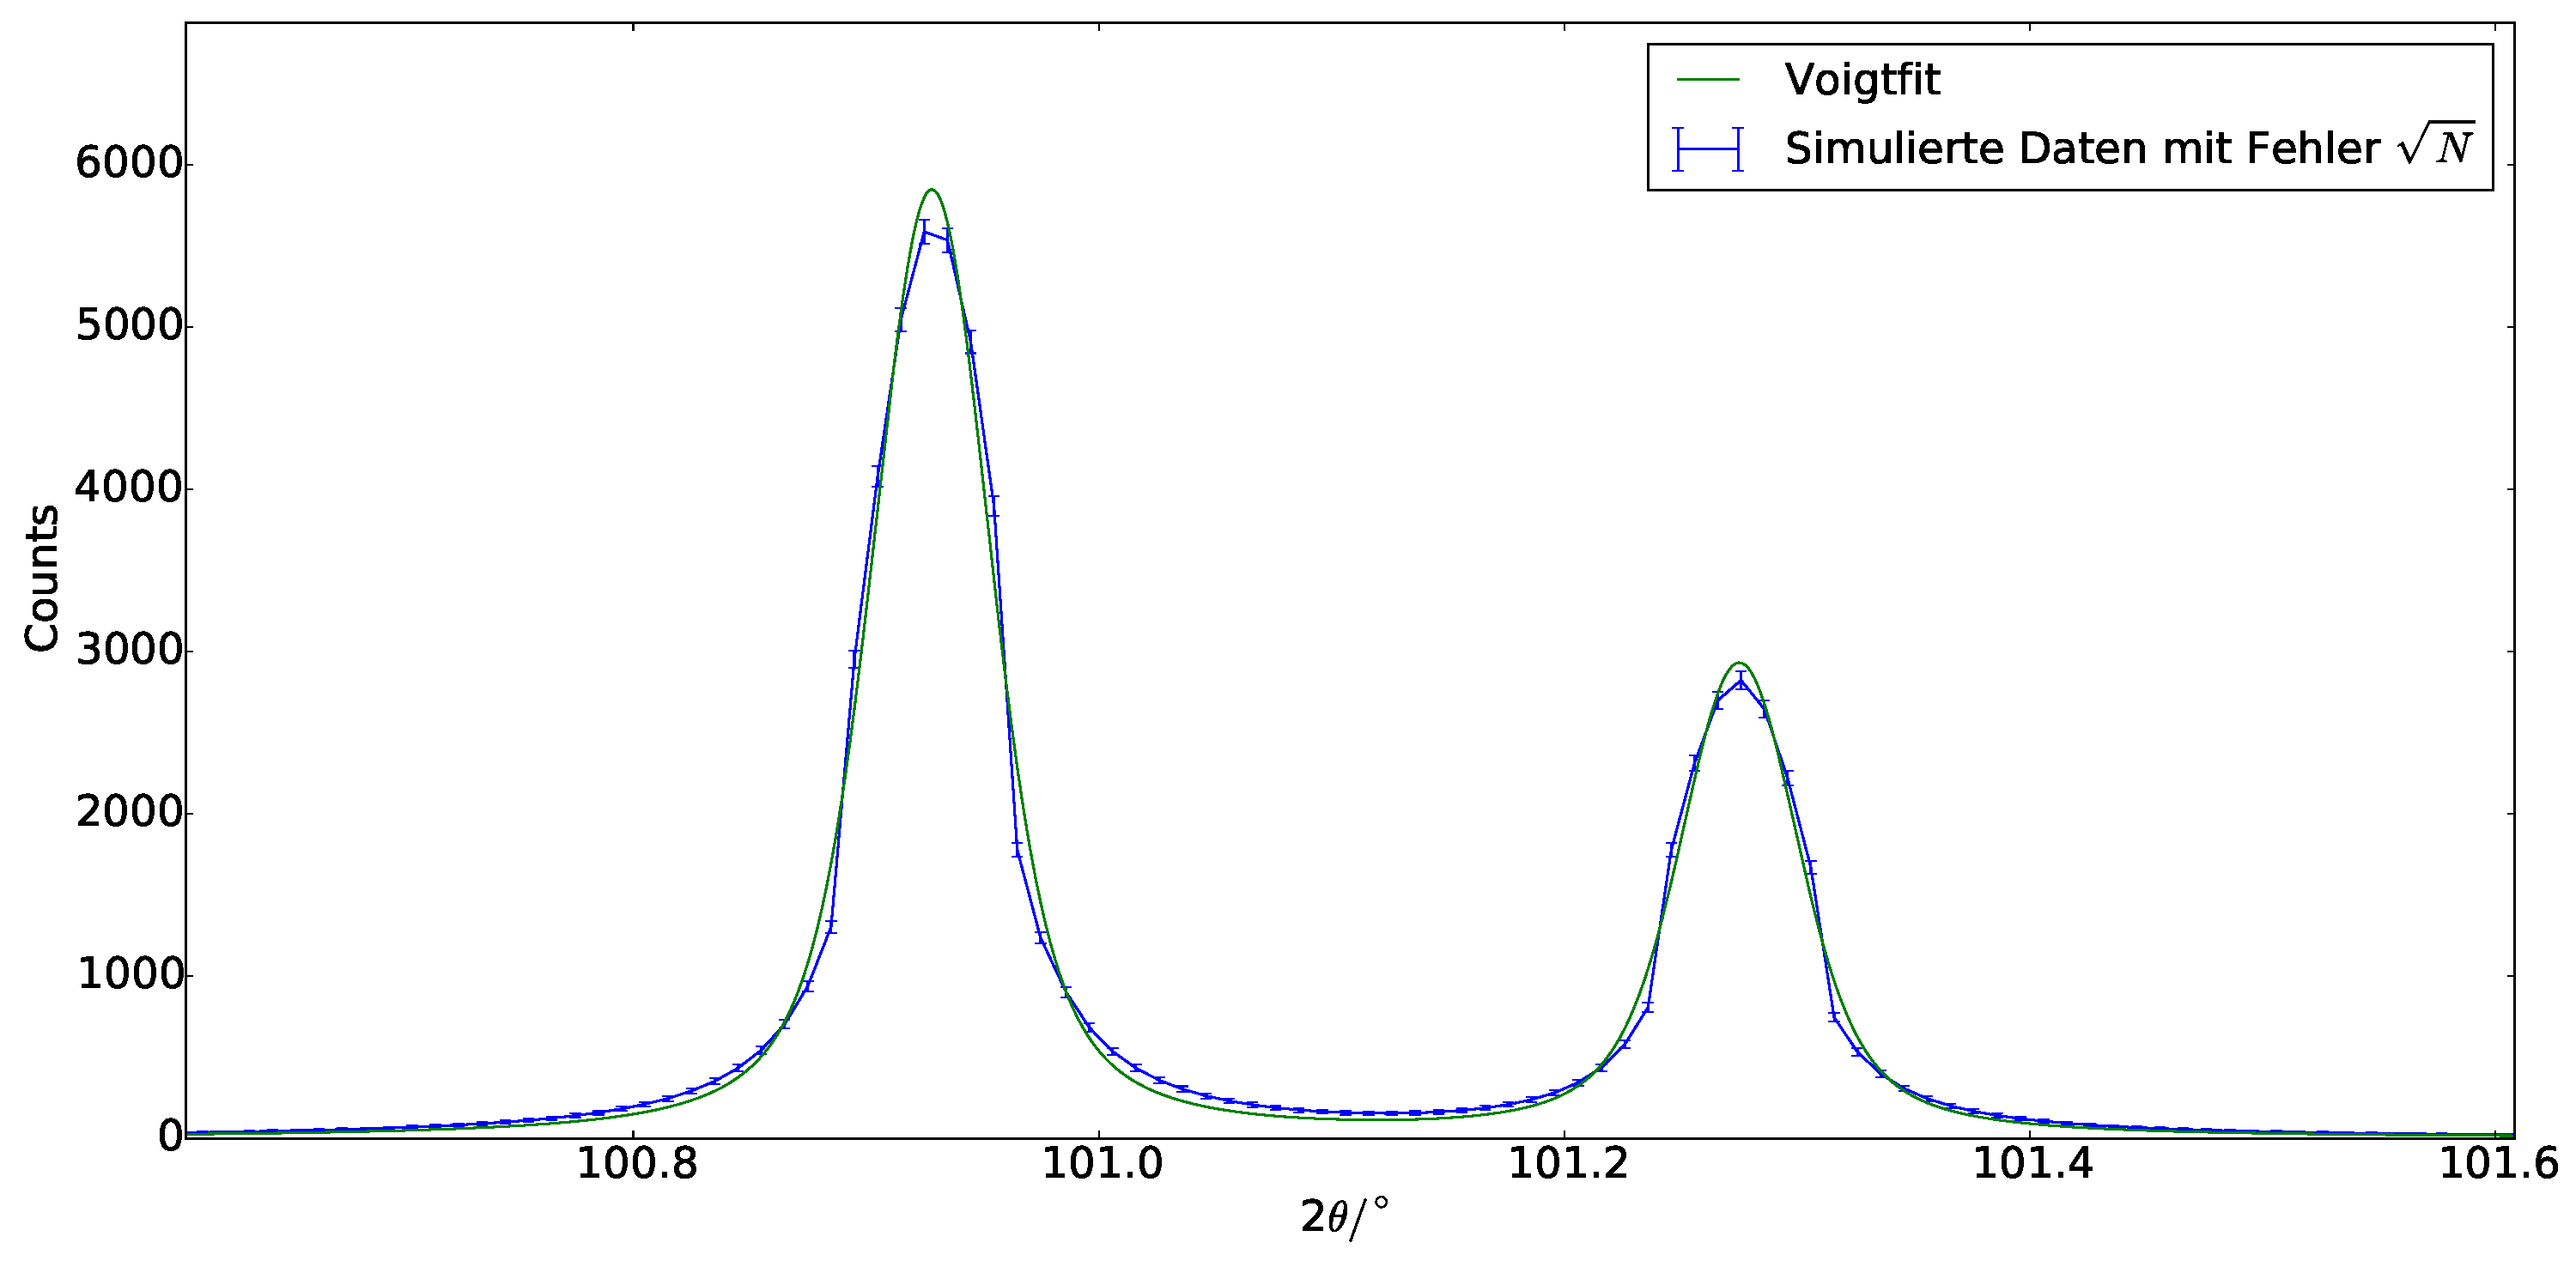
\includegraphics[scale=0.15]{Simulation_Germaniumpulver_8}
  \captionof{figure}{Germaniumpulver 8. Doppelpeak}
  \label{fig:pul_sim_ger_8}
\end{minipage}
\end{figure}
\begin{figure}[H]
\begin{minipage}{.5\textwidth}
  \centering
  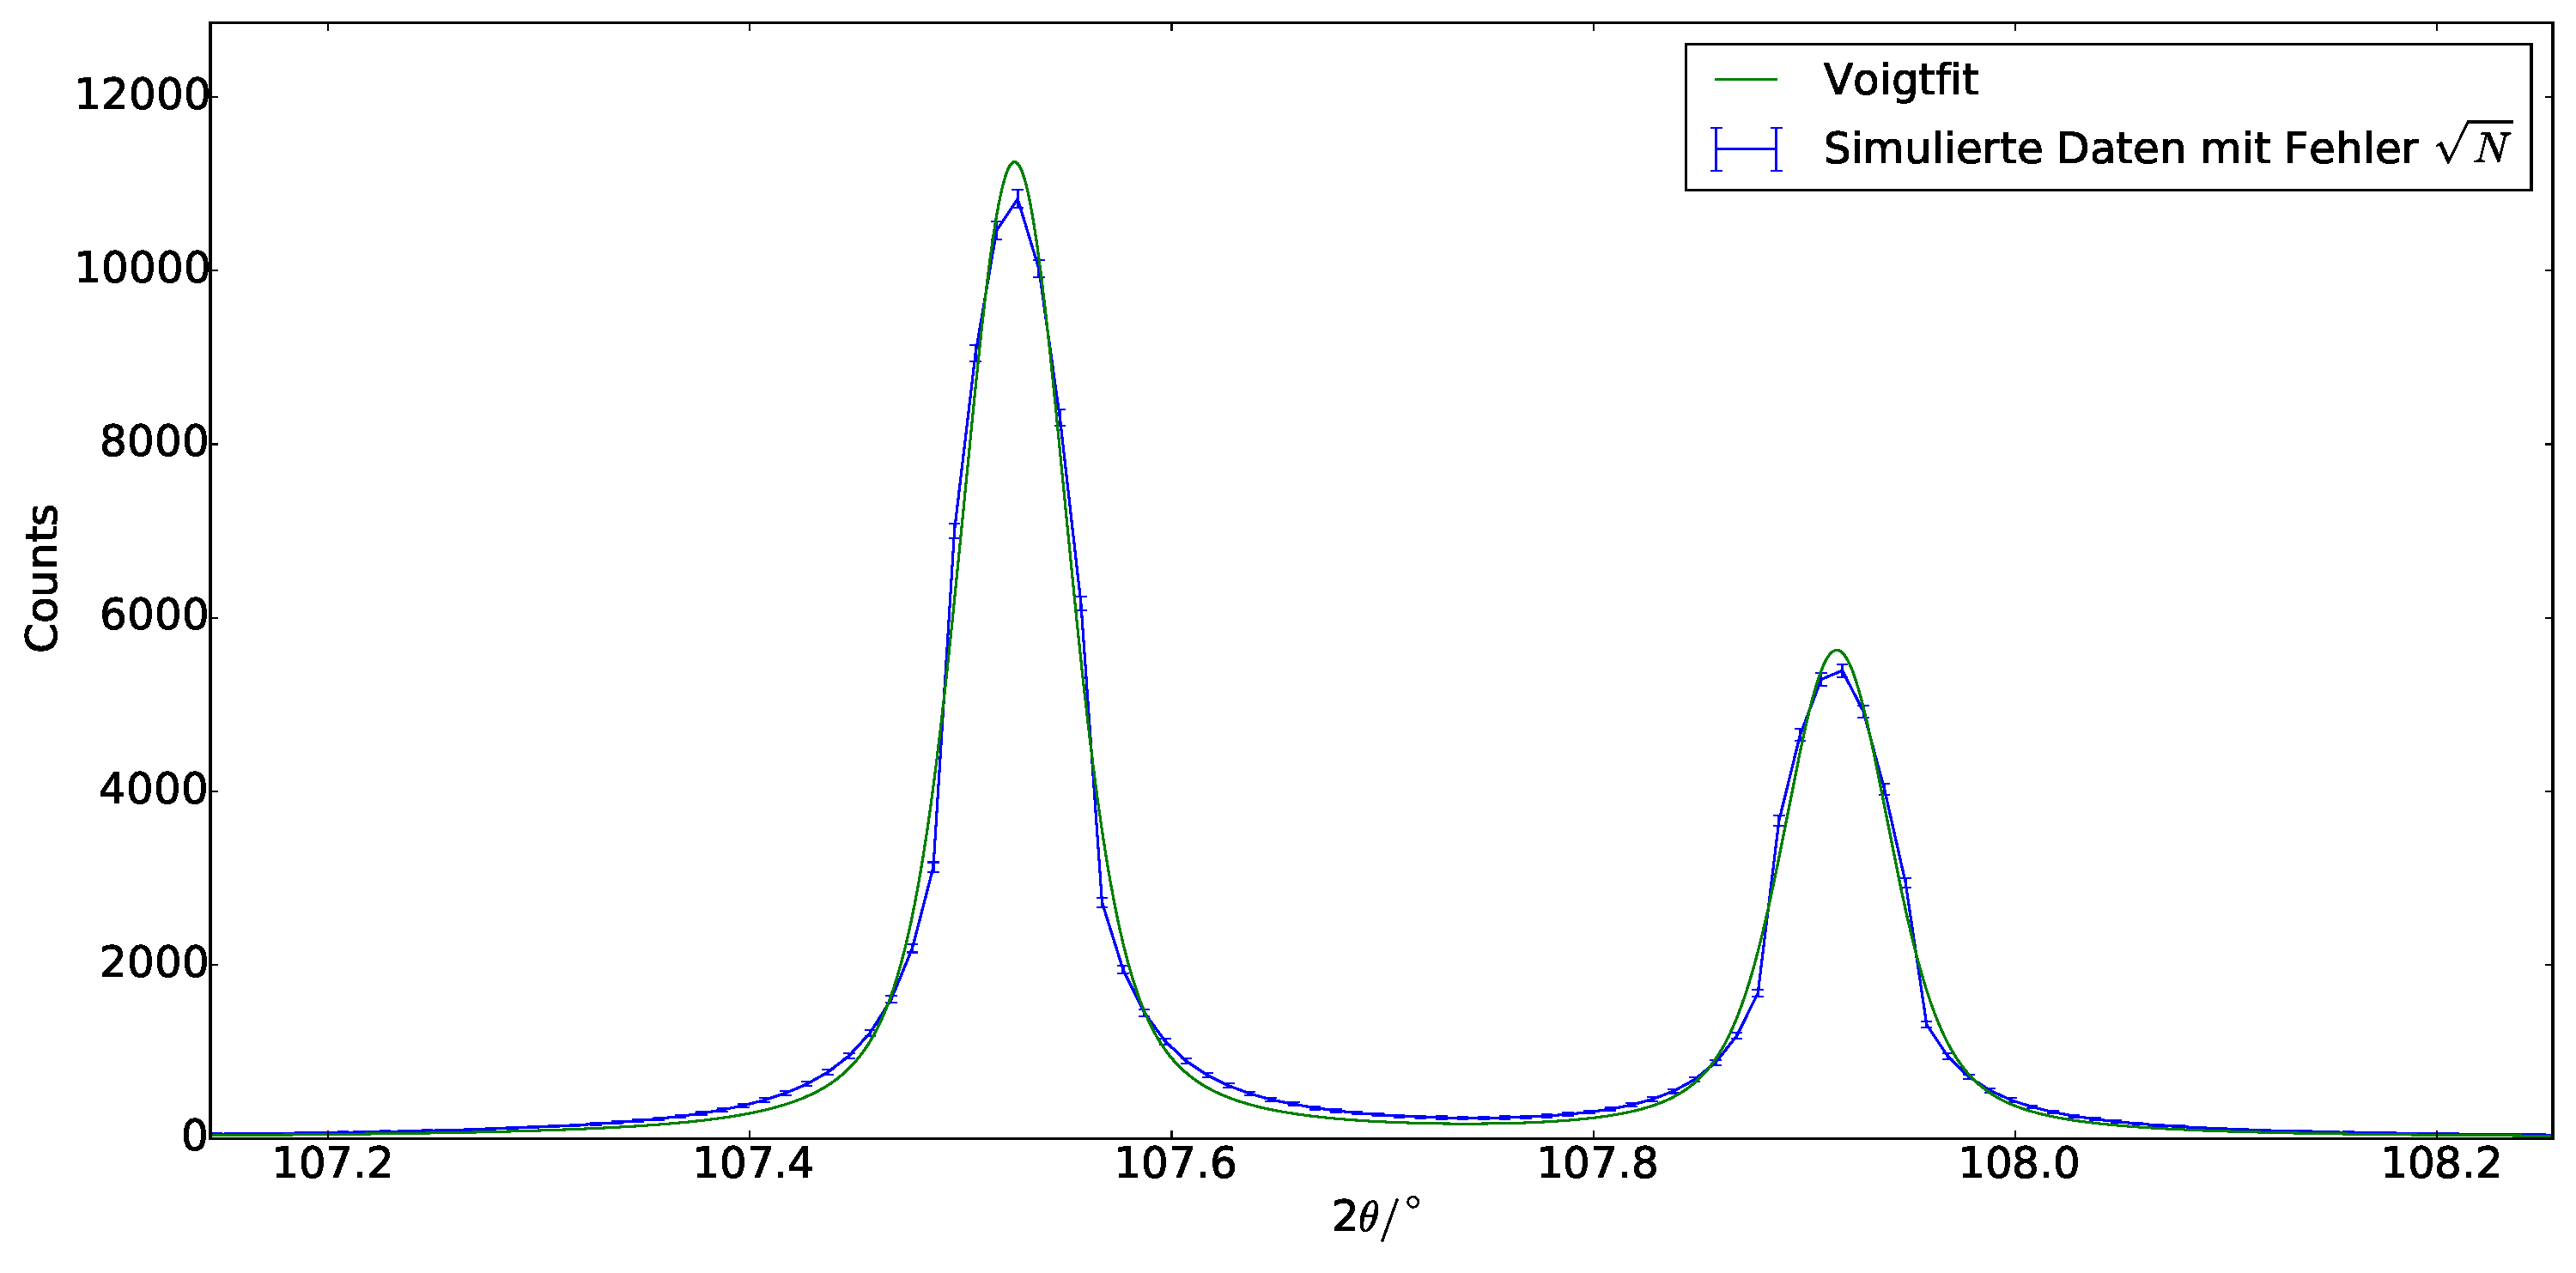
\includegraphics[scale=0.15]{Simulation_Germaniumpulver_9}
  \captionof{figure}{Germaniumpulver 9. Doppelpeak}
  \label{fig:pul_sim_ger_9}
\end{minipage}
\hspace{0.5cm}
\begin{minipage}{.5\textwidth}
  \centering
  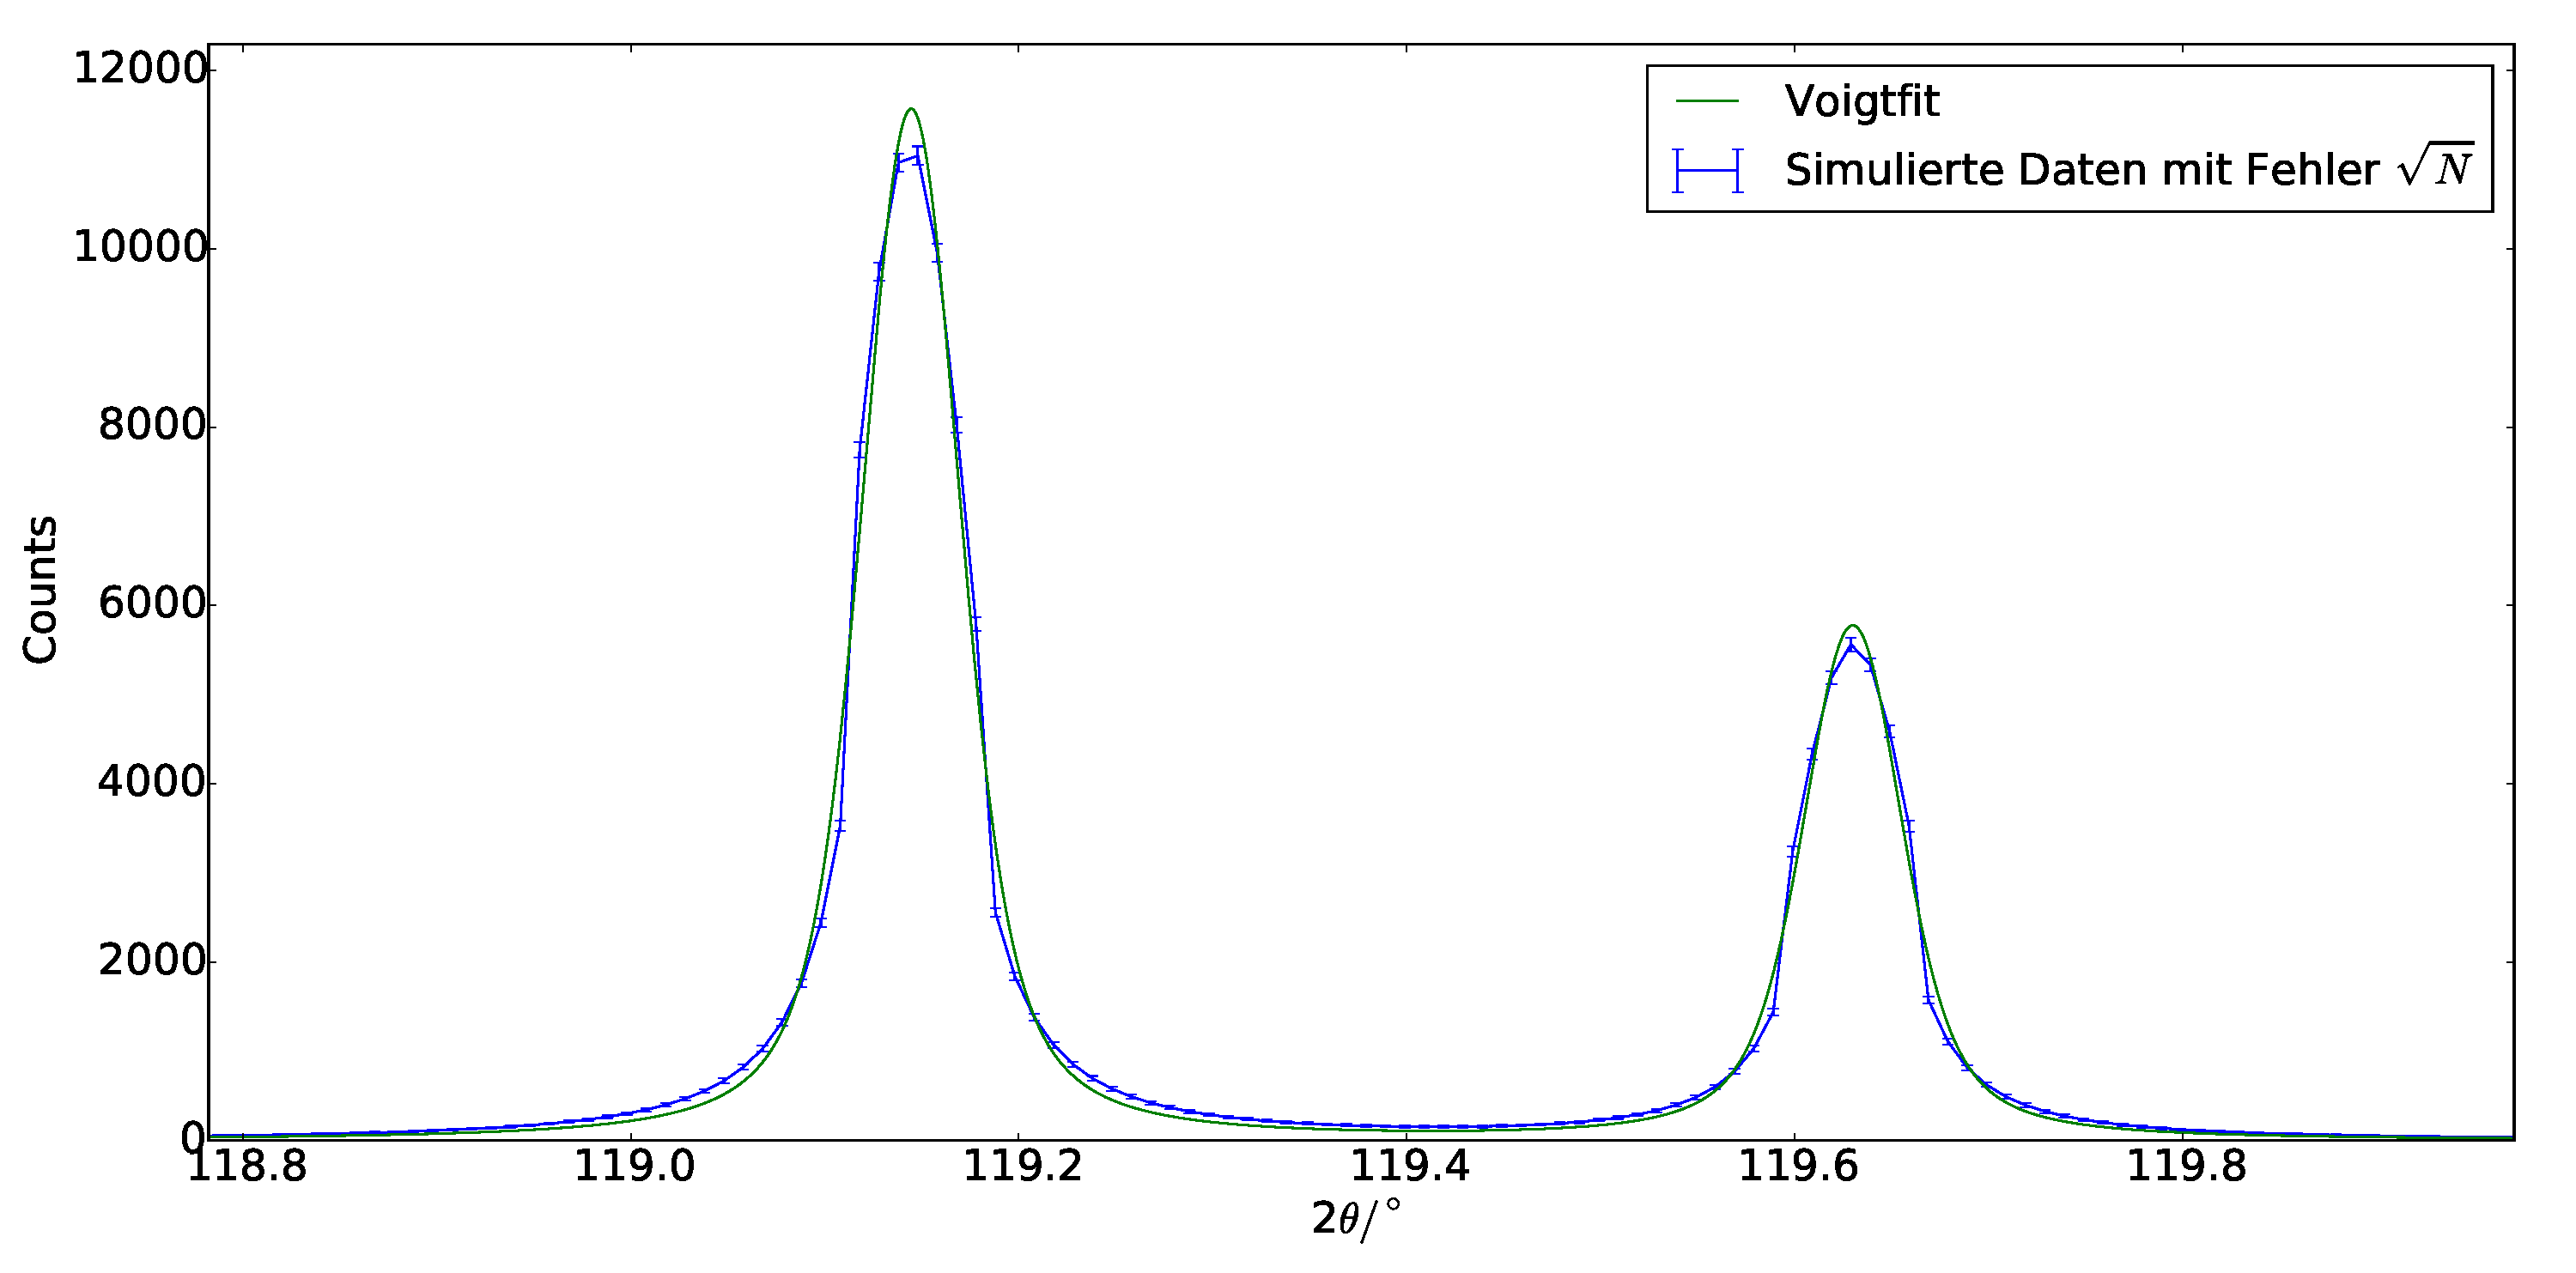
\includegraphics[scale=0.15]{Simulation_Germaniumpulver_10}
  \captionof{figure}{Germaniumpulver 10. Doppelpeak}
  \label{fig:pul_sim_ger_10}
\end{minipage}
\end{figure}
\begin{figure}[H]
\begin{minipage}{.5\textwidth}
  \centering
  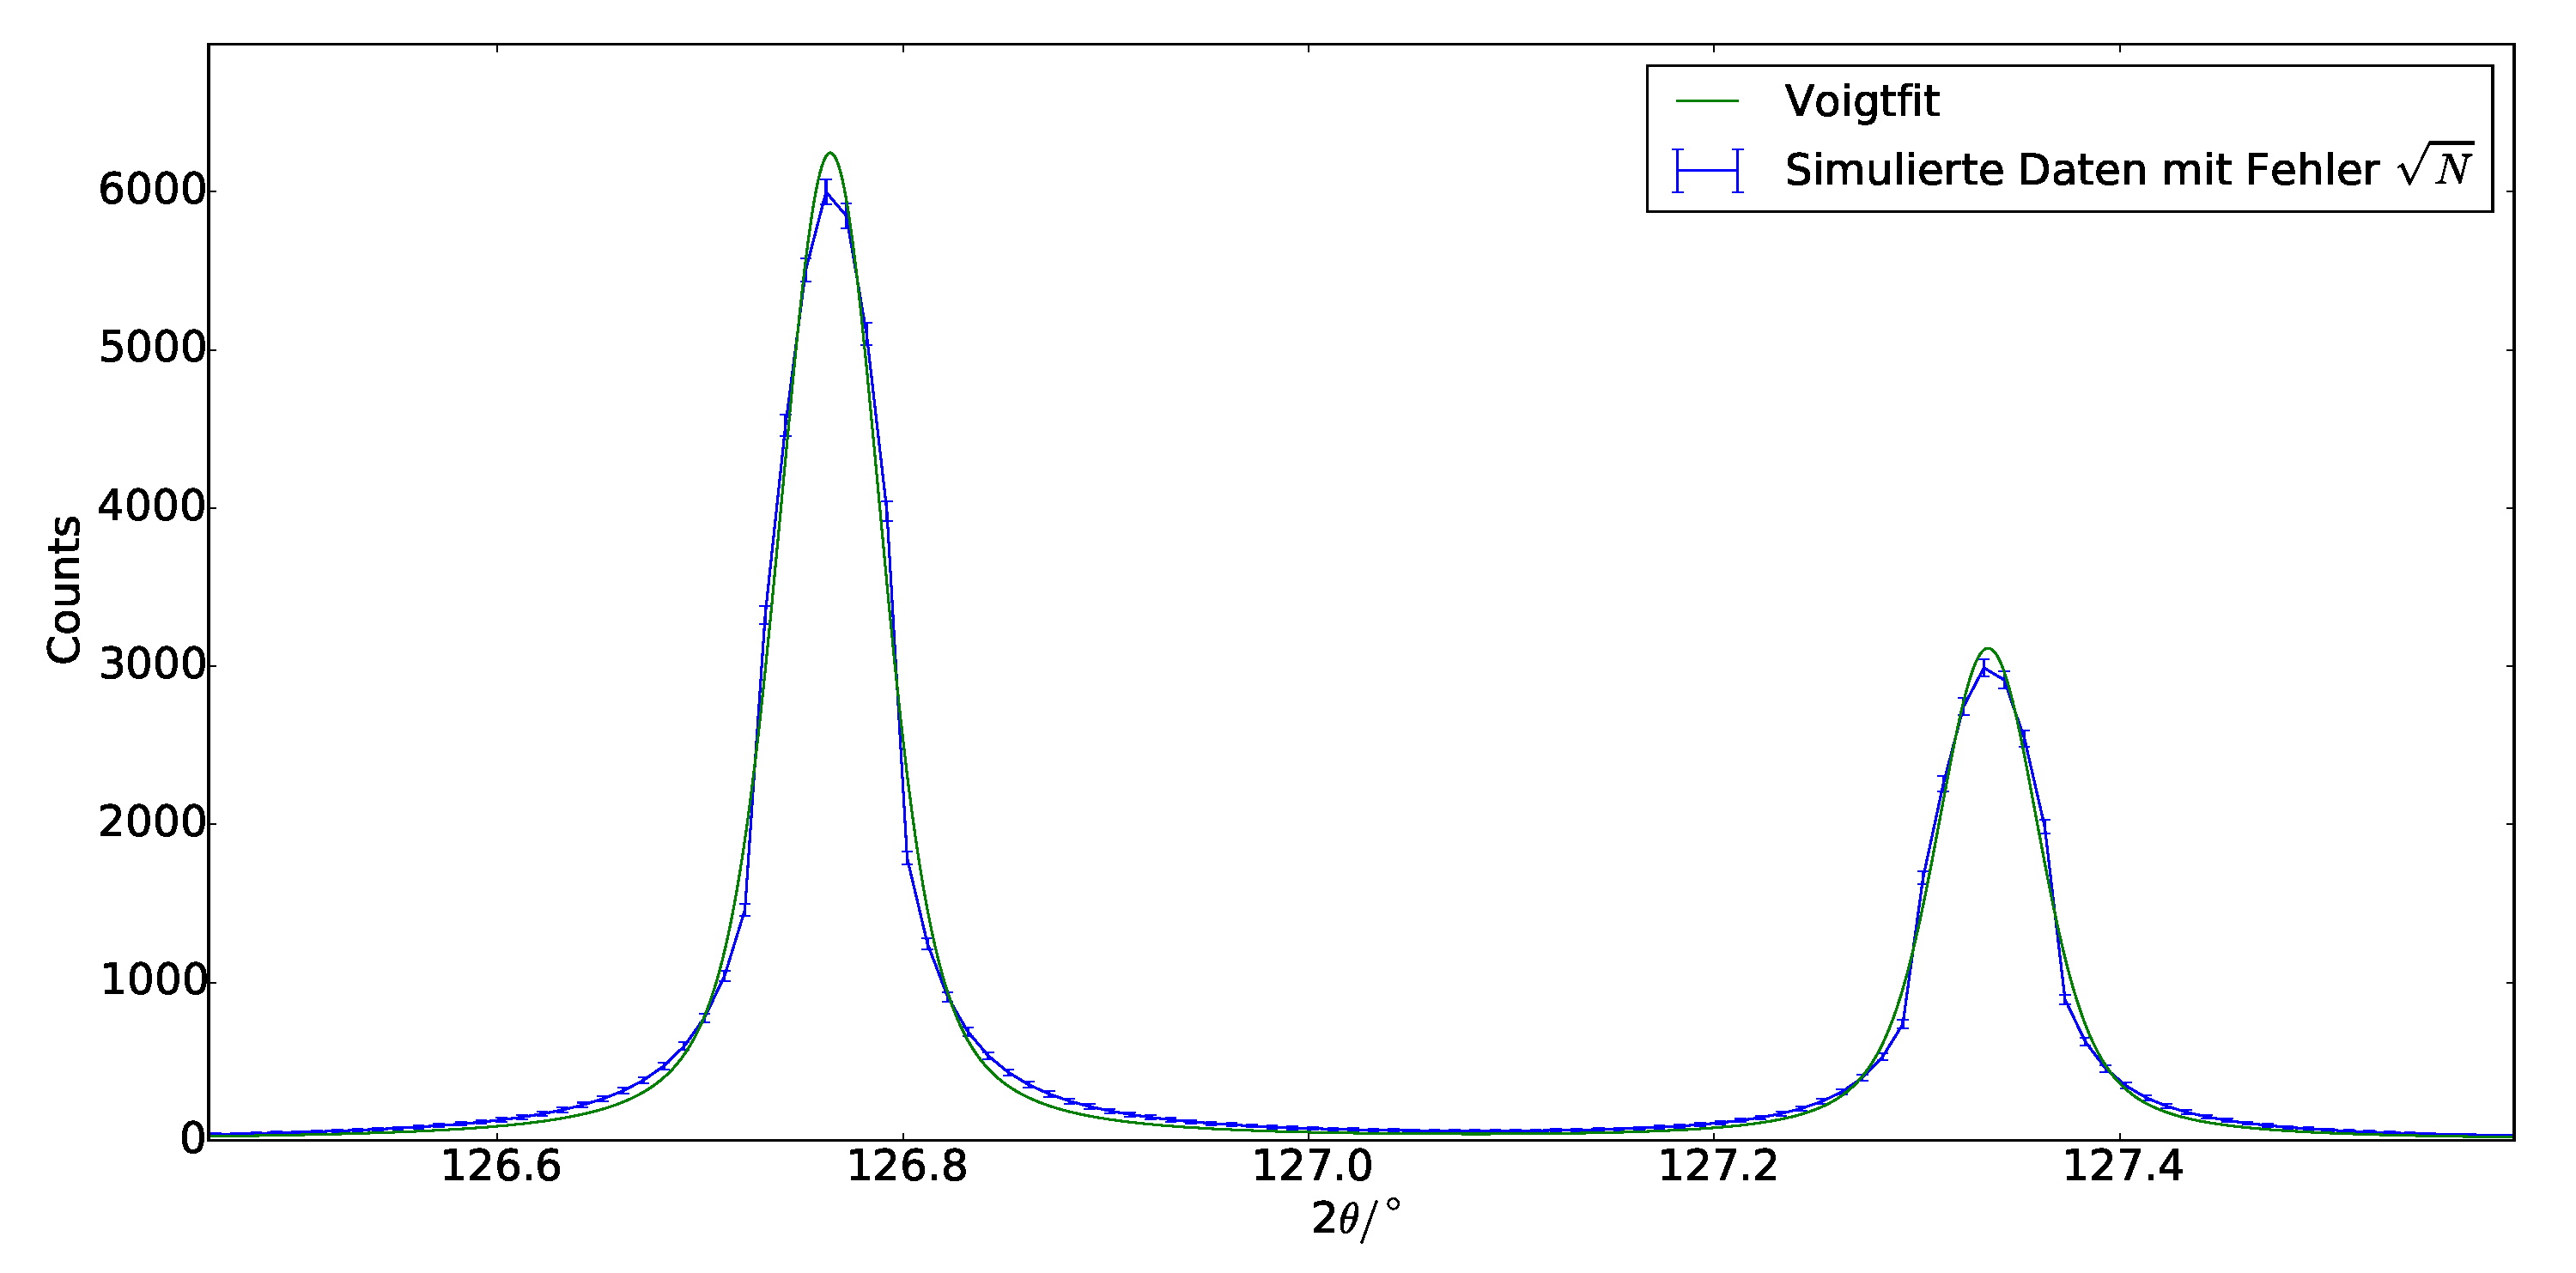
\includegraphics[scale=0.15]{Simulation_Germaniumpulver_11}
  \captionof{figure}{Germaniumpulver 11. Doppelpeak}
  \label{fig:pul_sim_ger_11}
\end{minipage}
\end{figure}
